\documentclass[english, a4paper]{article}

\usepackage{amsmath, amssymb, amsthm} % AMS-TEX because of course.
\usepackage{mathtools}        % Load for, amongst other things, paired delimiters.
\usepackage{mathrsfs}         % Load for \mathscr font.
\usepackage{etoolbox}         % Load to be able to perform conditional tests in macros.
\usepackage{enumitem}         % Load for more customisable enumerate environments. Specifically better labels.
\usepackage{hyperref}         % Make the table of contents easier to navigate with hyperlinks.
\usepackage{thmtools}         % Load to enable end-of-example marks.
\usepackage{bm}               % We want bold, italicised maths for vectors.
\usepackage{makeidx}          % We want a pretty index to keep track of all the ideas.
\usepackage{tocbibind}        % Include index and bibliography in table of contents.
\usepackage{abstract}         % Load in order to more easily manipulate the appearance of abstracts.
\usepackage{fancyhdr}         % Use to customise the headings to include useful navigation information.
\usepackage{titlesec}         % Use to add 'Lecture' in front of section headings.
\usepackage[titles]{tocloft}  % Use to add same in front of sections in the table of contents.
\usepackage{pgfplots}         % Used for producing pretty graphs of functions.
\usepackage{wrapfig}          % Used for producing figures in within the text.
\usepackage{float}            % Force Here placement of floats.
\usepackage{subcaption}       % Used for subfigures.
\usepackage{siunitx}          % We sometimes want nicely formatted large numbers and SI units.
\usepackage{adjustbox}        % Help us center very wide tables.

% Make pgfplots stop complaining about possible issues.
\pgfplotsset{compat = 1.13}

% Since we'll want to draw areas under curves.
\usepgfplotslibrary{fillbetween}
\usetikzlibrary{patterns}

% Externalise TikZ, because some plots are quite heavy.
\usepgfplotslibrary{external}
\tikzexternalize

% Define arrow heads in TikZ that are centred on the endpoints.
\usetikzlibrary{arrows}
\makeatletter
\pgfarrowsdeclare{center*}{center*}
{
  \pgfarrowsleftextend{+-.5\pgflinewidth}
  \pgfutil@tempdima=0.4pt%
  \advance\pgfutil@tempdima by.2\pgflinewidth%
  \pgfarrowsrightextend{4.5\pgfutil@tempdima}
}
{
  \pgfutil@tempdima=0.4pt%
  \advance\pgfutil@tempdima by.2\pgflinewidth%
  \pgfsetdash{}{+0pt}
  \pgfpathcircle{\pgfqpoint{4.5\pgfutil@tempdima}{0bp}}{4.5\pgfutil@tempdima}
  \pgfusepathqfillstroke
}

\pgfarrowsdeclare{centero}{centero}
{
  \pgfarrowsleftextend{+-.5\pgflinewidth}
  \pgfutil@tempdima=0.4pt%
  \advance\pgfutil@tempdima by.2\pgflinewidth%
  \pgfarrowsrightextend{4.5\pgfutil@tempdima}
}
{
  \pgfutil@tempdima=0.4pt%
  \advance\pgfutil@tempdima by.2\pgflinewidth%
  \pgfsetdash{}{+0pt}
  \pgfpathcircle{\pgfqpoint{4.5\pgfutil@tempdima}{0bp}}{4.5\pgfutil@tempdima}
  \pgfusepathqstroke
}
\makeatother

% Let us draw pretty angles.
\usetikzlibrary{quotes, angles}

% Define a command for drawing circle arcs in TikZ.
\tikzset{
  pics/circle arc/.style args={#1:#2:#3}{
    code={
      \draw[pic actions] (#1:#3) arc(#1:#2:#3);
    }
  }
}

% Make headings
\pagestyle{headings}

% Remove the section number from the section name in headers.
\renewcommand{\sectionmark}[1]{\uppercase{\markboth{#1}{#1}}}

% Same in table of contents.
\renewcommand{\cftsecpresnum}{Lecture\space}
\newlength\lecturelength
\settowidth\lecturelength{\cftsecpresnum}
\addtolength\cftsecnumwidth{\lecturelength}

\setlength\intextsep{0pt}

% Label sections as 'lecture 1', etc.
\titleformat{\section}{\normalfont\Large\bfseries}{Lecture \thesection}{1em}{}

% Start indexing
\makeindex

% Change name of table of contents
\renewcommand{\contentsname}{Table of Contents}

% Remove the Abstract title from the abstract.
\renewcommand{\abstractname}{}    % Clear the title
\renewcommand{\absnamepos}{empty} % Originally centre

% Define a footnote macro that doesn't leave a mark.
\makeatletter
\def\blfootnote{\gdef\@thefnmark{}\@footnotetext}
\makeatother

% Define some common variously styled letters we occasionally need.
\newcommand{\C}{\ensuremath{\mathbb{C}}}
\newcommand{\Q}{\ensuremath{\mathbb{Q}}}
\newcommand{\R}{\ensuremath{\mathbb{R}}}
\newcommand{\Z}{\ensuremath{\mathbb{Z}}}
\newcommand{\N}{\ensuremath{\mathbb{N}}}
\newcommand{\Ll}{\ensuremath{\mathscr{Ll}}}
\newcommand{\D}{\ensuremath{\mathcal{D}}}
\newcommand{\Hh}{\ensuremath{\mathcal{H}}}

% Allow overwriting of \Re and \Im.
\let\Re\relax
\let\Im\relax
% Redefine \Re and \Im as Re and Im instead of mathfrak letters.
\DeclareMathOperator{\Re}{Re}
\DeclareMathOperator{\Im}{Im}

% Declare an image symbol
\DeclareMathOperator{\im}{im}

% Define a placeholder for functions without arguments.
\newcommand*{\placeholder}{\makebox[1ex]{\textbf{$\cdot$}}}


% Define a plethora of theorem/definition/lemma/etc. environments.
% Number them all using the same counter.
\newtheorem{theorem}{Theorem}[subsection]
\newtheorem*{theorem*}{Theorem}
\newtheorem{corollary}[theorem]{Corollary}
\newtheorem{lemma}[theorem]{Lemma}
\newtheorem{proposition}[theorem]{Proposition}
\newtheorem{conjecture}[theorem]{Conjecture}
\theoremstyle{definition}
\newtheorem{definition}[theorem]{Definition}
\newtheorem{definitions}[theorem]{Definitions}
\newtheorem{notation}[theorem]{Notation}
\newtheorem{axiom}[theorem]{Axiom}
\newtheorem{exercise}[theorem]{Exercise}
\newtheorem{exercises}[theorem]{Exercises}
\newtheorem{problem}[theorem]{Problem}
\theoremstyle{remark}
\newtheorem{remark}[theorem]{Remark}


% Define special example(s) and solution(s) environments in order to have end-of-environment marks.
\declaretheorem[
	style = definition,
	qed = $\blacktriangle$,
	sibling = theorem
]{example}
\declaretheorem[
	style = definition,
	qed = $\blacktriangle$,
	sibling = theorem
]{examples}

\declaretheorem[
	style = definition,
	qed = $\blacktriangle$,
	sibling = theorem
]{counterexample}

\declaretheorem[
	style = remark,
	qed = $\blacklozenge$,
	numbered = no
]{solution}
\declaretheorem[
	style = remark,
	qed = $\blacklozenge$,
	numbered = no
]{solutions}


% Number all equations and figures within subsections.
\numberwithin{equation}{subsection}
\numberwithin{figure}{subsection}

% Define some fake (i) label macros.
\newcommand{\fakeitemref}[1]{% \fakeitem{<n>}
	{\upshape(\emph{\romannumeral 0#1})}}
\newcommand{\fakeitem}[1]{% \fakeitem{<n>}
	\fakeitemref{#1}~}

% Make text both bold and emphasised, for keywords in definitions and similar.
\newcommand{\keyword}[1]{% \keyword{text}
	{\textbf{\emph{#1}}}}


% Redefine \overline to the nicely semantic \conjugate.
\newcommand*{\conjugate}[1]{\overline{#1}}



% For all of the below, use \command* to make the delimiters adjust size automatically.

% Defines an absolute value notation. Give it no argument and it'll default to \abs{\placeholder}.
\DeclarePairedDelimiterX{\abs}[1]{\lvert}{\rvert}{% \abs{a}
	\ifblank{#1}{\placeholder}{#1}%
}

% Provide semantic notation for describing sets with conditions.
\providecommand\given{} % Just make sure this exists, so that things don't explode.
\DeclarePairedDelimiterX{\Set}[1]{\{}{\}}{% \Set{ x \given x > 0}
	\,\renewcommand\given{\nonscript\:\delimsize\vert\nonscript\:\mathopen{}}#1\,
}

% Roman numerals
\makeatletter
\newcommand*{\rom}[1]{\expandafter\@slowromancap\romannumeral #1@}
\makeatother


% Alias for \section with optional footnote for date.
\newcommand{\lecture}[2][]{% \lecture{Name}{Date}
	\section[#2]{#2\ifblank{#1}{}{\footnote{Date: #1.}}}%
}

% Alias for \subsection that is more semantic.
\newcommand{\topic}{\subsection}

% Aliases for enumerate with certain label settings preapplied.
\newenvironment{romanlist}{\begin{enumerate}[label = \textup{(\emph{\roman*})}]}{\end{enumerate}}
\newenvironment{alphalist}{\begin{enumerate}[label = \textup{(\alph*)}]}{\end{enumerate}}



\title{Lecture Notes in Calculus I}
\author{Lectures by Jakob Streipel\thanks{\href{mailto:jakob.streipel@lnu.se}{jakob.streipel@lnu.se}}}
\date{}

\begin{document}
% Use Roman numberals for page numbers for frontmatter.
\pagenumbering{roman}

\maketitle

\begin{abstract}
	\noindent
	These lecture notes are based on the first few chapters of Robert A. Adams's \emph{Calculus: A Complete Course}, \cite{Adams2013}, wherein recommended exercises are also found. All the material covered can be found in there, though the exposition might sometimes be altered. Occasionally there will be small sections marked as `exercise.' These are examples or simpler proofs which are left for the student to think about on their own.  \blfootnote{Last updated \today.}

	\vspace{1em}

	\noindent
	Throughout this document, $\qed$ signifies end proof, and $\blacktriangle$ signifies end of example.%, and $\blacklozenge$ signifies end of solution.
\end{abstract}

\tableofcontents

% Begin mainmatter, and therefore use Arabic page numbering.
\cleardoublepage
\pagenumbering{arabic}

% Start at lecture 0
\setcounter{section}{-1}

\lecture[January 16, 2017]{Distance and Functions}

%!TEX root = ../lectures.tex

\topic{The Absolute Value and the Triangle Inequality}

Calculus is the art of using distances to measure changes in things (functions, typically).
Since we so far in our mathematical careers live on the real number line (which we denote $\R$)\index{real numbers}, the distance of choice is the absolute value:

\begin{definition}[Absolute value]
	Given a real number $x$, its \keyword{absolute value}\index{absolute value}, denoted $\abs{x}$, is defined as
	\[
		\abs{x} = \begin{cases}
		x, & \text{if}~ x \geq 0 \\
		-x, & \text{if}~ x < 0,
		\end{cases}
	\]
	i.e. $x$ without its sign.
\end{definition}

\noindent
In a very real sense Calculus (at least in the modern treatment of the subject) always boils down to manipulating this distance in sufficiently clever ways.
To this end, we will spend a bit of time recalling some basic properties of the absolute value.

The absolute value behaves well under multiplication and division.
In particular, we have that for all real $x$
\[
	\abs{-x} = \abs{x},
\]
for all real $x$ and $y$ we have
\[
	\abs{x y} = \abs{x} \abs{y},
\]
and for all real $x$ and $y$, where $y \neq 0$, we have
\[
	\abs*{\frac{x}{y}} = \frac{\abs{x}}{\abs{y}}.
\]

\begin{exercise}
	Prove the three properties listed above.
\end{exercise}

\noindent
On the other hand, the absolute value does not behave quite as well under addition and subtraction.
Indeed, we can't guarantee that we maintain equality anymore!

\begin{theorem}[The triangle inequality]\index{triangle inequality}
	Let $x$ and $y$ be real numbers. Then
	\[
		\abs{x + y} \leq \abs{x} + \abs{y}.
	\]
\end{theorem}

\noindent
There are many, many ways to prove this.
This is one of them:

\begin{proof}
	Consider the following equalities:
	\[
		\abs{x + y}^2 = (x + y)^2 = x^2 + 2 x y + y^2.
	\]
	Now suppose that we replace $x$ with $\abs{x}$ and $y$ with $\abs{y}$.
	Clearly the squares are unchanged since they're both nonnegative regardless of the sign of $x$ or $y$, but the middle term might change.
	If one of $x$ and $y$ is negative, we've made the sum bigger by replacing them with their absolute values, and in every other case we've changed nothing.
	Therefore
	\[
		\abs{x + y}^2 = x^2 + 2 x y + y^2 \leq \abs{x}^2 + 2 \abs{x} \abs{y} + \abs{y}^2.
	\]
	But this last expression we recognise as $(\abs{x} + \abs{y})^2$, whence $\abs{x + y}^2 \leq (\abs{x} + \abs{y})^2$.
	By taking (positive) square roots, we get the desired result.
\end{proof}

\noindent
Note that $\abs{x - y} \leq \abs{x} + \abs{y}$ holds by almost exactly the same argument, which might come in handy later on.

We will find that the triangle inequality is \emph{the} main tool in all of this Calculus course, which is why we bother with repeating this.

As an exercise in using the triangle inequality, let us consider the following related version of it:

\begin{example}[The reverse/inverse triangle inequality]
	If $x$ and $y$ be real numbers, then
	\[
		\abs{x - y} \geq \abs[\big]{\abs{x} - \abs{y}}.
	\]
	To see this, consider first the following consequence of the basic properties we discussed above:
	\[
		\abs{x - y} = \abs{-(y - x)} = \abs{-1} \cdot \abs{y - x} = \abs{y - x}.
	\]

	\noindent
	Therefore by adding and subtracting the same thing (a trick that will appear again and again throughout this course) and using the triangle inequality we have
	\[
		\abs{x} = \abs{(x - y) + y} \leq \abs{x - y} + \abs{y},
	\]
	which if we subtract $\abs{y}$ from both sides becomes $\abs{x} - \abs{y} \leq \abs{x - y}$.
	Similarly, if we start with $\abs{y}$, we get $\abs{y} - \abs{x} \leq \abs{y - x}$, which if we multiply both sides by $-1$ gives us $\abs{x} - \abs{y} \geq - \abs{x - y}$.

	Combining these two we have $- \abs{x - y} \leq \abs{x} - \abs{y} \leq \abs{x - y}$, which if we take absolute values everywhere means that $\abs[\big]{\abs{x} - \abs{y}} \leq \abs{x - y}$.
\end{example}

\topic{Functions and Some of Their Properties}

Since we will spend the next few weeks concerning ourselves with how functions change and what the area underneath their graphs are and so on, it behooves us to define, once and for all, what we mean by a function.

\begin{definition}[Function, domain, codomain, and range]
	A \keyword{function}\index{function} $f$ on a set $X$ into a set $Y$ is a rule that assigns exactly one element $y \in Y$ to each $x \in X$.
	We use the notation $f \colon X \to Y$ for the function together with the two sets.
	We use $y = f(x)$ to denote this unique $y$ corresponding to $x$.

	The set $X$ is called the \keyword{domain}\index{domain} of the function and the set $S$ is called its \keyword{codomain}\index{codomain}.
	By \keyword{range}\index{range} or \keyword{image}\index{image|see {range}} we mean the set $\Set{y = f(x) \given x \in X} \subseteq Y$ containing all elements of $Y$ that we may reach using the function $f$ on its domain $D$.
\end{definition}

\noindent
Note that a function strictly speaking depends on its domain and codomain, not just the formula expressing how we translate an element in the domain to an element in the codomain.

For example, the functions $f \colon \R \to \R$, $f(x) = x^2$ and $g \colon \R_{\geq 0} \to \R_{\geq 0}$, $g(x) = x^2$ (where we by $\R_{\geq 0}$ mean the nonnegative real numbers) are identical for $x \geq 0$, but $f(-1) = 1$, whereas $g(-1)$ is undefined.

If we do not specify the domain of a function, we implicitly give the function its \keyword{natural domain}\index{domain!natural}, by which we mean all $x \in \R$ such that $f(x) \in \R$, i.e. as big a subset of $\R$ as possible.
Similarly when we don't specify the codomain we take it to be the range of the function.

As an example it is then understood that the function $h(x) = \sqrt{x}$ has the set $\R_{\geq 0}$ both as its domain and its codomain.

For two additional properties of functions, suppose that we have a function $f \colon X \to Y$ such that $-x \in X$ whenever $x \in X$.

We call such a function \keyword{even}\index{function!even} if $f(-x) = f(x)$ for all $x$ in $X$, and we call it \keyword{odd}\index{function!odd} if $f(-x) = - f(x)$ for all $x$ in $X$.

Some odd functions are, for instance, $f_1(x) = x$ and $f_2(x) = \sin(x)$. For even functions, consider perhaps $f_3(x) = \abs{x}$ or $f_4(x) = \cos(x)$.
Note that most functions are neither even nor odd, say for example $f_5(x) = 2x + 3$.



\lecture[January 17, 2017]{Limits}

%!TEX root = ../lectures.tex

\topic{Informal Introduction}

Consider a function such as
\[
	f(x) = \frac{2x + 5}{7 - 3x},
\]
defined for all $x \neq 7/3$. What happens if we plug in \emph{big} values of $x$? It is then (perhaps) natural to consider $2x$ to be the bigger term of the numerator, and similarly $-3x$ the bigger term in the denominator.
Thus
\[
	f(x) \approx \frac{2x}{-3x} = \frac{2}{-3} = - \frac{2}{3}
\]
for \emph{big} values of $x$.

On the other hand for $x$ near $0$, the dominating terms are $5$ and $7$ in the numerator and denominator respectively, whereby
\[
	f(x) \approx \frac{5}{7}
\]
for $x$ near $0$.

To describe these two circumstances we introduce the notation
\[
	\lim_{x \to \infty} f(x) = - \frac{2}{3} \qquad \text{and} \qquad \lim_{x \to 0} f(x) = \frac{5}{7},
\]


\noindent
read as ``the \keyword{limit}\index{limit} as $x$ goes to infinity of $f(x)$,'' and similarly for the second one. We call $\infty$ and $0$ \keyword{limit points}\index{limit point}.

Of course the ``dominating'' argument isn't rigorous\ldots We need proper definition and rules of computation.
For instance,
\[
	\lim_{x \to \infty} f(x) = \lim_{x \to \infty} \frac{2x + 5}{7 - 3x} = \lim_{x \to \infty} \frac{x (2 + 5/x)}{x (7/x - 3)} = \lim_{x \to \infty} \frac{2 + 5/x}{7/x - 3} = \frac{2 + 0}{0 - 3} = - \frac{2}{3}.
\]

\begin{figure}
	\centering
	\begin{tikzpicture}
		\begin{axis}[
			scale = 1,
			axis x line = middle,
			axis y line = middle,
			xmin = -5,
			xmax = 15,
			ymin = -5,
			ymax = 5,
			xlabel = $x$,
			ylabel = $y$,
			restrict y to domain = -10:10,
			every axis x label/.style = {
				at = {(ticklabel* cs:1.01)},
				anchor = west,
			},
			every axis y label/.style = {
				at = {(ticklabel* cs:1.01)},
				anchor = south,
			},
			]
			\addplot[
			black,
			smooth,
			domain = -5:2.332
			]{(2*x+5)/(7-3*x)};
			\addplot[
			black,
			smooth,
			domain = 2.334:15
			]{(2*x+5)/(7-3*x)};
		\end{axis}
	\end{tikzpicture}
	\caption{Plot of $y = f(x)$.}
	\label{lec1:plotf(x)}
\end{figure}

\noindent
Moreover, by studying the plot of the function in Figure \ref{lec1:plotf(x)}, we might observe two more interesting limits, namely
\[
	\lim_{x \to 7/3^+} f(x) = +\infty \quad \text{and} \quad \lim_{x \to 7/3^+} f(x) = -\infty,
\]
where by the superscript $-$ and $+$ mean that the values of $x$ approach $7/3$ either from below or from above.
We call the first limit a \keyword{left limit}\index{limit!left} and the second a \keyword{right limit}\index{limit!right}.

We will spend the remainder of this lecture formalising what we mean by these limits and creating computational rules for them, informed by the intuition of what we do above.

\topic{Punctured or Deleted Neighbourhoods}

If we wish to study what happens to a function close to some point (or off at infinity), it is first of all important that our function is defined around this point.
More specifically, we require (at least in this course) that the function is defined \emph{for all} $x$ in \emph{some} \keyword{deleted} or \keyword{punctured neighbourhood}\index{deleted neighbourhood}\index{punctured neighbourhood|see {deleted neighbourhood}} of the limit point.

We will explain what we mean by this by means of examples.

\begin{example}
	For all real $\gamma > 0$ the set
	\[
		\Set{x \in \R \given 0 < \abs{x - 6} < \gamma}
	\]
	is a \keyword{two-sided deleted neighbourhood} of $x = 6$.
	Deleted naturally means that the point $x = 6$ itself is excluded.

	Drawn on the number line it looks something like this.

	\begin{figure}[H]
		\centering
		\begin{tikzpicture}
			\draw[latex-latex] (-1.5, 0) -- (8.5, 0);
			\foreach \x in {-1, 0, 1, 2, 3, 4, 5, 6, 7, 8}
			\draw[shift = {(\x, 0)}, color = black] (0pt, 3pt) -- (0pt, -3pt);
			\foreach \x in {-1, 0, 1, 2, 3, 4, 5, 6, 7, 8}
			\draw[shift = {(\x, 0)}, color = black] (0pt, 0pt) -- (0pt, -3pt) node[below] {$\x$};
			\draw[centero-centero] (5.2, 0) node[above] {$6 - \gamma$} -- (6, 0);
			\draw[-centero] (6, 0) -- (6.8, 0) node[above] {$6 + \gamma$};
			\draw[very thick] (5.2, 0) -- (6, 0);
			\draw[very thick] (6, 0) -- (6.8, 0);
		\end{tikzpicture}
	\end{figure}
\end{example}

\begin{example}
	For right limits we instead consider \keyword{deleted right neighbourhoods}, like
	\[
		\Set{ x \in \R \given 0 < x - 5 < \gamma} = \Set{ x \in \R \given 5 < x < 5 + \gamma} = {]{5, 5 + \gamma}[},
	\]
	around the point $x = 5$ for all real $\gamma > 0$.

	\begin{figure}[H]
		\centering
		\begin{tikzpicture}
			\draw[latex-latex] (-1.5, 0) -- (8.5, 0);
			\foreach \x in {-1, 0, 1, 2, 3, 4, 5, 6, 7, 8}
			\draw[shift = {(\x, 0)}, color = black] (0pt, 3pt) -- (0pt, -3pt);
			\foreach \x in {-1, 0, 1, 2, 3, 4, 5, 6, 7, 8}
			\draw[shift = {(\x, 0)}, color = black] (0pt, 0pt) -- (0pt, -3pt) node[below] {$\x$};
			\draw[centero-centero] (5, 0) -- (6.3, 0) node[above] {$5 + \gamma$};
			\draw[very thick] (5, 0) -- (6.3, 0);
		\end{tikzpicture}
	\end{figure}

	\noindent
	Similarly for left limits we use \keyword{deleted left neighbourhoods} such as the following for $x = 3$:
	\[
		\Set{ x \in \R \given 0 < 3 - x < \gamma} = \Set{ x \in \R \given 3 - \gamma < x < 3} = {]{3 - \gamma, 3}[}.
	\]

	\begin{figure}[H]
		\centering
		\begin{tikzpicture}
			\draw[latex-latex] (-1.5, 0) -- (8.5, 0);
			\foreach \x in {-1, 0, 1, 2, 3, 4, 5, 6, 7, 8}
			\draw[shift = {(\x, 0)}, color = black] (0pt, 3pt) -- (0pt, -3pt);
			\foreach \x in {-1, 0, 1, 2, 3, 4, 5, 6, 7, 8}
			\draw[shift = {(\x, 0)}, color = black] (0pt, 0pt) -- (0pt, -3pt) node[below] {$\x$};
			\draw[centero-centero] (1.2, 0) node[above] {$3 - \gamma$} -- (3, 0);
			\draw[very thick] (1.2, 0) -- (3, 0);
		\end{tikzpicture}
	\end{figure}
\end{example}

\noindent
For limits at infinity (or negative infinity) we also need a deleted neighbourhood to work with, but they looks rather different.

\begin{example}
	A \keyword{deleted neighbourhood of infinity} consists of all $x$ bigger than some fixed $A \in \R$,
	\[
		\Set{x \in \R \given x > A} = {]{A, \infty}[}.
	\]

	\begin{figure}[H]
		\centering
		\begin{tikzpicture}
			\draw[latex-latex] (-1.5, 0) -- (8.5, 0);
			\foreach \x in {-1, 0, 1, 2, 3, 4, 5, 6, 7, 8}
			\draw[shift = {(\x, 0)}, color = black] (0pt, 3pt) -- (0pt, -3pt);
			\foreach \x in {-1, 0, 1, 2, 3, 4, 5, 6, 7, 8}
			\draw[shift = {(\x, 0)}, color = black] (0pt, 0pt) -- (0pt, -3pt) node[below] {$\x$};
			\draw[centero-] (3, 0) node[above] {$A$} -- (8.5, 0);
			\draw[very thick,-latex] (3, 0) -- (8.5, 0);
		\end{tikzpicture}
	\end{figure}

	\noindent
	For a \keyword{deleted neighbourhood of negative infinity}, we instead take all $x$ smaller than some fixed $A \in \R$.
\end{example}

\topic{Definition of Limit}

We will now take the final steps toward a good definition of a limit.

\fakeitem{1} First of all we need the function we are studying to be defined \emph{around} the point of interest, i.e. the limit point.
This is the reason we are interested in deleted neighbourhoods around points!
In other words, for some function $f \colon X \to Y$ we need there to exist some $\gamma > 0$ such that the deleted neighbourhood
\[
	\Set{x \in \R \given 0 < \abs{x - a} < \gamma} \subseteq X,
\]
meaning that the function is defined somewhere around the limit point $a$.

\begin{remark}
	Note that the function needn't be defined at the limit point itself for us to study limits at this point.
\end{remark}

\begin{figure}
	\centering
	\begin{tikzpicture}[scale = 1]
		\begin{axis}[
			axis x line = left,
			axis y line = left,
			xmin = -2,
			xmax = 10,
			ymin = -2,
			ymax = 10,
			ticks = none,
			xlabel = $x$,
			ylabel = $y$,
			restrict y to domain = -2:10,
			every axis x label/.style = {
				at = {(ticklabel* cs:1.01)},
				anchor = west,
			},
			every axis y label/.style = {
				at = {(ticklabel* cs:1.01)},
				anchor = south,
			},
			]
			\addplot[
			black,
			smooth,
			domain = -2:10,
			]{-0.2*(x-4)^3-0.03*(x-4)^2+4.5};
		\end{axis}
		\draw[centero-centero] (3.5, 0) node[below] {$a - \delta$} -- (4, 0);
		\draw[-centero] (4, 0) node[above] {$a$} -- (4.5, 0) node[below] {$a + \gamma$};
		\draw[very thick] (3.5, 0) -- (4, 0);
		\draw[very thick] (4, 0) -- (4.5, 0);
		\draw[dashed] (3.5, 0) -- (3.5, 5.5);
		\draw[dashed] (4.5, 0) -- (4.5, 5.5);
		\draw[centero-center*] (0, 2.3) node[left] {$L - \varepsilon$} -- (0, 3);
		\draw[-centero] (0, 3) node[right] {$L$} -- (0, 3.7) node[left] {$L + \varepsilon$};
		\draw[very thick] (0, 2.3) -- (0, 3);
		\draw[very thick] (0, 3) -- (0, 3.7);
		\draw[dashed] (0, 2.3) -- (5.5, 2.3);
		\draw[dashed] (0, 3.7) -- (5.5, 3.7);
	\end{tikzpicture}
	\caption{Constructing neighbourhoods around limit and limit point.}
	\label{lec1:epsilondelta}
\end{figure}

Secondly we want the $y$ in $y = f(x)$ to get \emph{arbitrarily} close to the limit, let's call it $L$.

What we mean by this is that we should be able to pick \emph{any} neighbourhood around $L$,
\[
	\abs{y - L} < \varepsilon
\]
for any $\varepsilon > 0$, and regardless of what $\varepsilon$ we choose, we should be able to arrange for a deleted neighbourhood around $a$,
\[
	\Set{x \in \R \given 0 < \abs{x - a} < \delta},
\]
such that for all $x$ in this deleted neighbourhood, $y = f(x)$ is in the above neighbourhood of $L$.
We present a sketch of what this looks like in Figure \ref{lec1:epsilondelta}.

Therefore,

\fakeitem{2} For each $\varepsilon > 0$ there exists some $\delta > 0$ such that if $0 < \abs{x - a} < \delta$, then $\abs{f(x) - L} < \varepsilon$.

In other words, if $x$ is within $\delta$ distance away from $a$, then $f(x)$ is within $\varepsilon$ distance away from $L$.

Combining these two we have a proper definition of a limit at a point:

\begin{definition}[Limit at a point]
	We say that the function $f \colon X \to Y$ has the \keyword{limit} $L$ as $x$ approaches $a$ if and only if
	\begin{romanlist}
		\item there exists some $\gamma > 0$ such that $\Set{x \in \R \given 0 < \abs{x - a} < \gamma} \subseteq X$, and
		\item for each $\varepsilon > 0$ there exists a number $\delta > 0$ such that for each $x \in X$ with $0 < \abs{x - a} < \delta$ we have $\abs{f(x) - L} < \varepsilon$.
	\end{romanlist}
\end{definition}

\noindent
We call this an ``epsilon-delta'' definition.

In order to construct definitions for limits at infinity, left or right limits, or \keyword{improper limits}\index{limit!improper} (meaning that $f(x)$ approaches positive or negative infinity), we simply replace our various neighbourhoods in the above definition by the corresponding types of neighbourhoods.
For example:

\begin{definition}[Limit at negative infinity]
	We say that $f \colon X \to Y$ has the limit $L$ as $x$ approaches $-\infty$ if and only if
	\begin{romanlist}
		\item there exists some $A \in \R$ such that $\Set{x \in \R \given x < A} \subseteq X$, and
		\item for each $\varepsilon > 0$ there exists a number $B \in \R$ such that for each $x \in X$ with $x < B$ we have $\abs{f(x) - L} < \varepsilon$.
	\end{romanlist}
\end{definition}

\begin{exercise}
	Feel free to construct definitions for the remaining types of limits.
	Alternatively, try modify the wording of the original definition by replacing all neighbourhoods with expressions like ``there exists a deleted neighbourhood around the point'', etc, whereby we may acquire a completely general definition (albeit maybe slightly less practical).
\end{exercise}

\noindent
The idea that limits concern themselves with deleted neighbourhoods around the limit point is important.
That is to say, we don't care about the function's value in the limit point, or even if it is defined there.
We illustrate this by example:

\begin{example}\label{lec1:linewithhole}
	Consider the function
	\[
		f(x) = \frac{x^2 - 1}{x - 1},
	\]
	defined for all $x \neq 1$. For all such $x$ we have
	\[
		f(x) = \frac{x^2 - 1^2}{x - 1} = \frac{(x + 1)(x - 1)}{x - 1} = x + 1,
	\]
	i.e. a straight line passing through $y = 1$, except it's undefined at $x = 1$, meaning that there's a hole there.

	\begin{figure}[H]
		\centering
		\begin{tikzpicture}
			\begin{axis}[
				scale = 1,
				axis x line = middle,
				axis y line = middle,
				xmin = -0.5,
				xmax = 3,
				ymin = -0.5,
				ymax = 4,
				xlabel = $x$,
				ylabel = $y$,
				every axis x label/.style = {
					at = {(ticklabel* cs:1.01)},
					anchor = west,
				},
				every axis y label/.style = {
					at = {(ticklabel* cs:1.01)},
					anchor = south,
				},
				]
				\addplot[
				black,
				smooth,
				domain = -1:3
				]{x+1};
				\addplot[mark = *, mark options = {fill = white}] coordinates {(1, 2)};
			\end{axis}
		\end{tikzpicture}
	\end{figure}

	\noindent
	Even though $f(x)$ is \emph{undefined} at $x = 1$, it is clear that we can make it as close to $y = 2$ as we like by taking $x$ sufficiently close to $x = 1$, i.e.
	\[
		\lim_{x \to 1} f(x) = 2.
	\]

	\noindent
	Formally, for any $\varepsilon > 0$ we want
	\[
		\abs{f(x) - 2} = \abs*{\frac{x^2 - 1}{x - 1} - 2} = \abs*{\frac{(x - 1)(x + 1) - 2 (x - 1)}{x - 1}} = \abs{x - 1} < \varepsilon
	\]
	whenever $\abs{x - 1} < \delta$, so by taking $\delta = \varepsilon$ we have proved formally that the limit is what we expect!
\end{example}

\begin{example}
	To further emphasise how the limit at a point doesn't care about the value of the function at that point, consider the following function, closely related to the one in the last example:
	\[
		f(x) = \begin{cases}
		\frac{x^2 - 1}{x - 1}, & \text{if}~ x \neq 1 \\
		3, & \text{if}~ x = 1.
		\end{cases}
	\]
	This function \emph{is} defined at $x = 1$, but even so, by the exact same computation as above, the limit at that point is still $2$.
\end{example}

\noindent
Finally in this section we will prove something quite important, that is sometimes overlooked:

\begin{theorem}
	Limits are unique.
\end{theorem}

\begin{proof}
	We will prove this in the case of a two-sided limit at a point, but the remaining types of limits follow by similar arguments.

	Suppose
	\[
		\lim_{x \to a} f(x) = L \qquad \text{and} \qquad \lim_{x \to a} f(x) = M.
	\]
	We want to prove that $L = M$.

	By definition we have that for any $\varepsilon > 0$, or, equivalently, for any $\varepsilon / 2 > 0$, there exists some $\delta_1$ such that whenever $\abs{x - a} < \delta_1$, it implies that $\abs{f(x) - L} < \varepsilon / 2$, and similarly there exists some $\delta_2$ such that if $\abs{x - a} < \delta_2$, then $\abs{f(x) - M} < \varepsilon / 2$. If we now let $\delta = \min\Set{\delta_1, \delta_2}$, then when $\abs{x - a} < \delta$, both of the above conditions are satisfied, so by adding and subtracting the same thing and using the triangle inequality we get
	\begin{align*}
		\abs{L - M} & = \abs{L - f(x) + f(x) - M} \leq \abs{L - f(x)} + \abs{f(x) - M}                                 \\
		            & = \abs{f(x) - L} + \abs{f(x) - M} < \frac{\varepsilon}{2} + \frac{\varepsilon}{2} = \varepsilon.
	\end{align*}
	Since $\varepsilon > 0$ is arbitrarily small, and $\abs{L - M}$ is smaller than every one of them, we must have that $\abs{L - M} = 0$, which means that $L = M$.
\end{proof}

\topic{Computing Limits}

We have used epsilon-delta explicitly to compute a limit in Example \ref{lec1:linewithhole}, but we will now use the same in the abstract to establish several general rules for how limits may be computed and manipulated.

\begin{theorem}[Computational rules for limits]
	Let $f$ and $g$ be some functions such that
	\[
		\lim_{x \to a} f(x) = L \qquad \text{and} \qquad \lim_{x \to a} g(x) = M.
	\]
	Moreover let $k \in \R$ be a constant. Then
	\begin{romanlist}
		\item $\displaystyle \lim_{x \to a} (f(x) + g(x)) = L + M$,
		\item $\displaystyle \lim_{x \to a} (f(x) - g(x)) = L - M$,
		\item $\displaystyle \lim_{x \to a} (k f(x)) = k L$,
		\item $\displaystyle \lim_{x \to a} (f(x)g(x)) = LM$,
		\item $\displaystyle \lim_{x \to a} \frac{f(x)}{g(x)} = \frac{L}{M}$, if $M \neq 0$,
		\item $\displaystyle \lim_{x \to a} (f(x))^{m/n} = L^{m/n}$ for $m, n \in \Z$, $n > 0$, $L > 0$ if $n$ is even, and $L \neq 0$ if $m < 0$, and finally
		\item if $f(x) \leq g(x)$ in a deleted neighbourhood around $a$, then $L \leq M$.
	\end{romanlist}
\end{theorem}

\begin{proof}
	We will prove some of them.
	First of all note that, since both $f$ and $g$ must be defined in some punctured neighbourhood of $a$, since they have limits there, the combined functions must as well.
	For example, if $f$ is defined for $0 < \abs{a - x} < \gamma_f$, and $g$ is defined for $0 < \abs{a - x} < \gamma_g$, then at the very least $f + g$ must be defined for $0 < \abs{a - x} < \min\Set{\gamma_f, \gamma_g}$.
	By this argument (and similar for the other limits), we find that we are allowed to use our limit definition on these new functions in the first place.

	The proof technique is invariably the same, in the sense that it boils down to choosing appropriate $\delta$.
	By definition, for all $\varepsilon_1, \varepsilon_2 > 0$ there exist some $\delta_1, \delta_2 > 0$ such that we have $\abs{f(x) - L} < \varepsilon_1$ whenever $\abs{x - a} < \delta_1$ and $\abs{g(x) - M} < \varepsilon_2$ whenever $\abs{x - a} < \delta_2$.

	\fakeitem{1} In order to verify that $L + M$ is the limit of $f(x) + g(x)$ as $x$ approaches $a$, we simply compute the distance between these two quantities:
	\begin{align*}
		\abs{f(x) + g(x) - (L + M)} & = \abs{(f(x) - L) + (g(x) - M)}                                       \\
		                            & \leq \abs{f(x) - L} + \abs{g(x) - M} < \varepsilon_1 + \varepsilon_2.
	\end{align*}
	Note the use of the triangle inequality.
	Taking $\varepsilon_1 = \varepsilon_2 = \varepsilon / 2$, with $\varepsilon > 0$ being arbitrary, and also taking $\delta = \min\Set{\delta_1, \delta_2}$, we have that whenever $\abs{x - a} < \delta$, we must have $\abs{(f(x) - g(x)) - (L - M)} < \varepsilon$, so by definition
	\[
		\lim_{x \to a} (f(x) + g(x)) = L + M.
	\]

	\fakeitem{4} First, the relation between $\varepsilon_2$ and $\delta_2$ is that for \emph{any} $\varepsilon_2$, there must exist a corresponding $\delta$, whereby it must in particular work if we take $\varepsilon_2 = 1$.
	Thus there exists a $\delta_3$ such that if $\abs{x - a} < \delta_3$, then $\abs{g(x) - M} < 1$.
	This means that
	\[
		\abs{g(x)} = \abs{g(x) - M + M} \leq \abs{g(x) - M} + \abs{M} < 1 + \abs{M}
	\]
	when $\abs{x - a} < \delta_3$.

	We now turn to the distance between $f(x)g(x)$ and $LM$,
	\begin{align*}
		\abs{f(x)g(x) - LM} & = \abs{f(x)g(x) - L g(x) + L g(x) - LM}                           \\
		                    & = \abs{(f(x) - L) g(x) + L(g(x) - M)}                             \\
		                    & \leq \abs{(f(x) - L) g(x)} + \abs{L (g(x) - M)}                   \\
		                    & = \abs{g(x)} \cdot \abs{f(x) - L} + \abs{L} \cdot \abs{g(x) - M},
	\end{align*}
	so if take let $\abs{x - a} < \min\Set{\delta_1, \delta_2, \delta_3}$ and take
	\[
		\varepsilon_1 = \frac{\varepsilon}{2 (1 + \abs{M})} \qquad \text{and} \qquad \varepsilon_2 = \frac{\varepsilon}{2 \abs{L}},
	\]
	then the above quantity is less than
	\[
		(1 + \abs{M}) \, \frac{\varepsilon}{2 (1 + \abs{M})} + \abs{L} \, \frac{\varepsilon}{2 \abs{L}} = \varepsilon,
	\]
	meaning that by definition
	\[
		\lim_{x \to a} (f(x)g(x)) = LM. \qedhere
	\]
\end{proof}

\noindent
Finally we present one more useful theoretical result before we use these computational rules in a few examples.

\begin{theorem}[Squeeze theorem]
	Suppose $f(x) \leq g(x) \leq h(x)$ holds for all $x$ in some deleted interval around a point $a$, and suppose further that
	\[
		\lim_{x \to a} f(x) = \lim_{x \to a} h(x) = L.
	\]
	Then
	\[
		\lim_{x \to a} g(x) = L
	\]
	as well.
\end{theorem}

\begin{proof}
	We have that for all $\varepsilon_1, \varepsilon_2 > 0$ there exist some $\delta_1, \delta_2 > 0$ such that $\abs{x - a} < \delta_1$ implies $\abs{f(x) - L} < \varepsilon_1$ and $\abs{x - a} < \delta_2$ implies $\abs{f(x) - L} < \varepsilon_2$.

	Let us now try to compute the distance between $g(x)$ and $L$:
	\[
		\abs{g(x) - L} = \abs{g(x) - f(x) + f(x) - L} \leq \abs{g(x) - f(x)} + \abs{f(x) - L}.
	\]
	Now since $g(x) \leq h(x)$ sufficiently close to $a$, this is bounded by
	\begin{align*}
		\abs{g(x) - L} & \leq \abs{g(x) - f(x)} + \abs{f(x) - L}                \\
		               & \leq \abs{h(x) - f(x)} + \abs{f(x) - L}                \\
		               & = \abs{h(x) - L - f(x) + L} + \abs{f(x) - L}           \\
		               & = \abs{(h(x) - L) - (f(x) - L)} + \abs{f(x) - L}       \\
		               & \leq \abs{h(x) - L} + \abs{f(x) - L} + \abs{f(x) - L}.
	\end{align*}
	If we then take $\varepsilon_1 = \varepsilon_2 = \varepsilon / 3$, the last line above is equal to $\varepsilon$ so long as $\abs{x - a} < \min\Set{\delta_1, \delta_2}$, which is what we wanted to prove.
\end{proof}

\begin{remark}
	Just like the uniqueness of limits, these last two theorems also hold for the other types of limits, with similar proofs.
\end{remark}

\begin{example}
	Suppose that $3 - x^2 \leq f(x) \leq 3 + x^2$ holds for all $x \neq 0$.
	Find the limit of $f(x)$ as $x$ tends to $0$.

	By our computational rules we have that
	\[
		\lim_{x \to 0} (3 - x^2) = \lim_{x \to 0} 3 - \lim_{x \to 0} x^2 = \lim_{x \to 0} 3 - \big ( \lim_{x \to 0} x \big )^2 = 3 - 0^2 = 3,
	\]
	and by almost identical computation $\lim\limits_{x \to 0} (3 + x^2) = 3$ as well. Therefore the Squeeze theorem applies, and thus $\lim\limits_{x \to 0} f(x) = 3$ as well.
\end{example}

\begin{example}
	Show that if $\lim\limits_{x \to a} \abs{f(x)} = 0$, then $\lim\limits_{x \to a} f(x) = 0$.

	To this end we observe that $-\abs{f(x)} \leq f(x) \leq \abs{f(x)}$, and $\lim\limits_{x \to a} \abs{f(x)} = 0$ implies that
	\[
		\lim_{x \to a} - \abs{f(x)} = - \lim_{x \to a} \abs{f(x)} = - 0 = 0,
	\]
	so by the Squeeze theorem
	\[
		\lim_{x \to a} f(x) = 0. \qedhere
	\]
\end{example}



\lecture[January 24, 2017]{Continuity}\label{lec3:continuity}

An important type of functions (their importance will be justified throughout the course) are ones that, in some sense, don't jump.
That is to say, when we draw their graph on a piece of paper, we (sort of) never need to lift the pen.

However it isn't entirely straight forward how to define this.
In order to move toward a good definition, we'll discuss two important special cases that cover most, but not all, of our needs.

\topic{Special Cases}

\subsubsection*{The domain is an open interval}

If a function $f$ has the domain
\[
	X = \Set{x \in \R \given b < x < c},
\]
for some fixed $b$ and $c$, then $f$ is said to be \keyword{continuous}\index{continuity} if and only if for all $a \in X$ we have
\[
	\lim_{x \to a} f(x) = f(a).
\]

\noindent
In other words, the function agrees with its limit at every point.

\subsubsection*{The domain is a closed interval}

If a function $f$ has the domain
\[
	X = \Set{x \in \R \given b \leq x \leq c},
\]
where $b$ and $c$ are some constants, then $f$ is said to be \keyword{continuous} if and only if the following are satisfied:
\begin{romanlist}
	\item for all interior points, i.e. $b < a < c$, we have $\lim\limits_{x \to a} f(x) = f(a)$,
	\item for the left endpoint $b$, we have $\lim\limits_{x \to b^+} f(x) = f(b)$, and
	\item for the right endpoint $c$, we have $\lim\limits_{x \to c^-} f(x) = f(c)$.
\end{romanlist}

\noindent
The reason for this distinction is hopefully intuitively clear: if we are at an endpoint of the closed interval, we can't hope to find a deleted two-sided neighbourhood around this point for which the function is defined, and therefore by definition it cannot have a two-sided limit at this point.
Even so we still want to have a notion of continuity at such a point, so effectively what we do is the following:

We investigate the continuity of a function point by point, in the way that is reasonable depending on the point and its surrounding:
\begin{itemize}
	\item If the function is defined in a two-sided neighbourhood around a point, we require that the two-sided limit exists and agrees with the function value.
	\item If the function is defined only in a right neighbourhood of the point, we (obviously?) require only that the right limit exists and equals the function value.
	\item Likewise is the function is defined only in a left neighbourhood, we require a left limit equal to the value of the function.
\end{itemize}

\noindent
Of course mathematicians don't like special cases if they can avoid them, so we attempt to construct a general definition motivated by this discussion.

\topic{Definition of Continuity}

\begin{definition}[Continuity in a point]
	We say that the function $f \colon X \to Y$ is \keyword{continuous in the point}\index{continuity}\index{continuity!point} $a \in \R$ if and only if the following two conditions are satisfied:
	\begin{romanlist}
		\item $a \in X$, and
		\item for each $\varepsilon > 0$ there exists a $\delta > 0$ such that, for all $x \in X$, we have that if $\abs{x - a} < \delta$, then $\abs{f(x) - f(a)} < \varepsilon$.
	\end{romanlist}
\end{definition}

\begin{remark}
	There is a crucial difference in this epsilon-delta construction compared to that of our limit definition, namely that we don't actually demand that the function is defined anywhere except for the point $a$ itself. However if the function happens to be defined outside of this point $a$, then we impose some restrictions on these exterior points!
	It is this distinction that captures the subtleties of the second special case above.

	One consequence of this is that a function defined in an isolated point, say $f \colon \Set{1} \to \Set{2}$, defined by $f(1) = 2$, is continuous at that point $x = 1$ (try to prove it using the above defintion!). This might seem strange, but it turns out to be a good property to have, that moreover agrees with much more abstract definitions of continuity found in the field of topology.
\end{remark}

\noindent
Another interesting takeaway from this definition is that in principle a function is \keyword{discontinuous}\index{discontinuity} (not continuous) in any point not in its domain. However, when we study a function as a whole, we will consider only points in the domain:

\begin{definition}[Continuity of a function]
	We say that the function $f \colon X \to Y$ is a \keyword{continuous function}\index{continuity!function} if and only if the function is continuous for all $x \in X$.
\end{definition}

\noindent
This means that there are functions which we call continuous, despite actually being discontinuous in one or more point; it's just that these points are outside of the domain!

\begin{figure}
	\centering
	\begin{tikzpicture}
		\begin{axis}[
			scale = 1,
			axis x line = middle,
			axis y line = middle,
			xmin = -2,
			xmax = 12,
			ymin = -10,
			ymax = 10,
			xlabel = $x$,
			ylabel = $y$,
			every axis x label/.style = {
				at = {(ticklabel* cs:1.01)},
				anchor = west,
			},
			every axis y label/.style = {
				at = {(ticklabel* cs:1.01)},
				anchor = south,
			},
			]
			\addplot[
			black,
			samples = 100,
			domain = -2:6.9,
			]{1/(x-7)};
			\addplot[
			black,
			samples = 100,
			domain = 7.1:12,
			]{1/(x-7)};
		\end{axis}
	\end{tikzpicture}
	\caption{Plot of $\displaystyle f(x) = \frac{1}{x - 7}$.}
\end{figure}

\begin{example}
	The function $f \colon \R \setminus \Set{7} \to \R$ defined by
	\[
		f(x) = \frac{1}{x - 7}
	\]
	is discontinuous at $x = 7$, but continuous for all other $x \in \R$.
	But because $x = 7$ doesn't belong to the domain, $f$ is a continuous function anyway!
\end{example}

\noindent
We started off talking about the graph of a continuous function sort of not having a jump.
Clearly, this isn't entirely true, as evidenced by this example.
So with what we now know in hand, a better (and also correct) characterisation is that a continuous function has a graph that has no jumps in any interval in its domain.

\topic{Continuous Functions}

Many functions we are familiar with are continuous.

\begin{examples}
	All polynomials are continuous, as are all rational functions, and all rational powers $x^{m/n}$, $m, n \in \Z$, $n \neq 0$.

	The trigonometric functions (sine, cosine, tangent, etc.) are all continuous.

	The absolute value $\abs{x}$ is continuous as well.
\end{examples}

\noindent
We can also combine continuous functions to get new continuous functions:

\begin{theorem}[Combining continuous functions]
	If both $f$ and $g$ are functions defined on some neighbourhood containing $c$ and both are continuous at $c$, then the following functions are continuous at $c$:
	\begin{romanlist}
		\item $f + g$ and $f - g$;
		\item $fg$;
		\item $k f$, where $k \in \R$ is a constant;
		\item $\displaystyle \frac{f}{g}$, provided $g(c) \neq 0$;
		\item $(f)^{1 / n}$, $n \in \Z$, provided $f(c) > 0$ if $n$ is even.
	\end{romanlist}
\end{theorem}

\begin{proof}
	We simply use the rules for calculating limits from the last lecture.
	For instance:
	\begin{align*}
		\lim_{x \to c} (f \pm g)(x) & = \lim_{x \to c} \big ( f(x) \pm g(x) \big ) = \lim_{x \to c} f(x) \pm \lim_{x \to c} g(x) \\
		                            & = f(c) \pm g(c) = (f \pm g)(c)
	\end{align*}
	and
	\[
		\lim_{x \to c} (fg)(x) = \lim_{x \to c} \big ( f(x)g(x) \big ) = \big ( \lim_{x \to c} f(x) \big ) \big ( \lim_{x \to c} g(x) \big ) = f(c) g(c) = (fg)(c).
	\]

	\noindent
	Note that for endpoints of closed intervals in the domains of the functions, we would of course have to replace the above by appropriate one-sided limits.
\end{proof}

\noindent
A trickier result to prove, but one that is extremely useful is the following:

\begin{theorem}
	If $f(g(x))$ is defined on some neighbourhood of $c$, and if $f$ is continuous at $L$, with
	\[
		\lim_{x \to c} g(x) = L,
	\]
	then
	\[
		\lim_{x \to c} f(g(x)) = f(L) = f \big ( \lim_{x \to c} g(x) \big ).
	\]

	\noindent
	Furthermore, if $g$ is continuous at $c$ (i.e. $L = g(c)$), then $f \circ g$ is continuous at $c$ as well:
	\[
		\lim_{x \to c} f(g(x)) = f(g(c)).
	\]
\end{theorem}

\begin{proof}
	Let $\varepsilon > 0$.
	Because we will need to keep track of whether we're in the domain of $f$ or $g$, we will denote them by $X_f$ and $X_g$, respectively.
	Further we use $X_{f \circ g}$ to refer to the domain of the composition.
	We now establish what we know from the assumptions in the theorem.

	Since $f$ is continuous at $L = \lim\limits_{x \to c} g(x)$, there exists some $\delta_1 > 0$ such that for all $y \in X_f$ with
	\[
		\abs[\big]{y - \underbrace{\lim_{x \to c} g(x)}_{= L}} < \delta_1,
	\]
	we have that
	\begin{equation}\label{lec3:fcontinuous}
		\abs[\Big]{f(y) - f \big ( \lim_{x \to c} g(x) \big ) } < \varepsilon.
	\end{equation}

	\noindent
	Moreover since $\lim\limits_{x \to c} g(x) = L$, there exists some $\delta_2 > 0$ such that for all $x \in X_g$ with $\abs{x - c} < \delta_2$ we have $\abs{g(x) - L} < \delta_1$.

	We take a moment to point out what happened in the very last step there: in the definition of the limit of $g$, we are able to take \emph{any} $\varepsilon$, so in particular we can fix it to a specific value, namely $\delta_1$, and find a corresponding $\delta_2$ which makes the definition work.

	If we now take $x \in X_{f \circ g}$ such that $\abs{x - c} < \delta_2$, then $\abs{g(x) - L} < \delta_1$, so by the construction of $\delta_1$, Equation \eqref{lec3:fcontinuous} with $y = g(x)$ becomes
	\[
		\abs{f(g(x)) - f(L)} = \abs[\Big]{f(g(x)) - f \big ( \lim_{x \to c} g(x) \big )} < \varepsilon,
	\]
	so $f \circ g$ is continuous at $x = c$.
\end{proof}

\noindent
This means that not only are many of the elementary functions we are used to continuous, but almost any conceivable combination of them are as well!

\topic{Removable Discontinuities}

Recalling how functions are by definition discontinuous at any point where they are undefined, it might sometimes be possible to therefore define a function at some point where it wasn't previously defined, in such a way that the new function is continuous.
We demonstrate this by example:

\begin{example}
	Recall the function
	\[
		f(x) = \frac{x^2 - 1}{x - 1}
	\]
	from Example \ref{lec2:linewithhole} in the previous lecture.
	It is not continuous over all of $\R$, since it isn't even defined in $x = 1$, but it can be redefined to become continuous everywhere.

	Since $\lim\limits_{x \to 1} f(x) = 2$, we \emph{define} a new function $F$ which is $F(x) = f(x)$ for all $x \neq 1$, and $F(1) = 2$, so
	\[
		F(x) = \begin{cases}
		\frac{x^2 - 1}{x - 1}, & \text{if}~ x \neq 1 \\
		2, & \text{if}~ x = 1
		\end{cases}
		= x + 1,
	\]
	which is continuous everywhere.
	In this case, $x = 1$ is said to be a \keyword{removable discontinuity}\index{discontinuity!removable}, and $F(x)$ is said to be a \keyword{continuous extension}\index{continuity!extension} of $f(x)$.
\end{example}

\topic{Continuous Functions on Closed, Finite Intervals}

Continuous functions defined on closed and finite intervals have a few special properties.

\begin{theorem}[Max-min theorem]\index{max-min theorem}
	If $f$ is continuous on the closed finite interval $[a, b]$, then there exists $p, q \in [a, b]$ such that for all $x \in [a, b]$ we have
	\[
		f(p) \leq f(x) \leq f(q).
	\]

	\noindent
	In other words, $f(p)$ is an global minimum of the function, attained on the point $x = p$, and $f(q)$ is an global maximum, at the point $x = q$.
\end{theorem}

\begin{figure}
	\centering
	\begin{tikzpicture}
		\begin{axis}[
			scale = 1,
			axis x line = middle,
			axis y line = middle,
			xmin = -1,
			xmax = 4,
			ymin = -2,
			ymax = 5,
			xlabel = $x$,
			ylabel = $y$,
			every axis x label/.style = {
				at = {(ticklabel* cs:1.01)},
				anchor = west,
			},
			every axis y label/.style = {
				at = {(ticklabel* cs:1.01)},
				anchor = south,
			},
			]
			\addplot[
			black,
			samples = 100,
			domain = 0.2:3,
			]{3+(x-3)^2*sin((x-3)r)};
			\addplot[mark=*] coordinates {(3, 3)} node[pin=150:{$f(q)$}]{} ;
			\addplot[mark=*] coordinates {(0.711, -0.945)} node[pin=-30:{$f(p)$}]{} ;
		\end{axis}
	\end{tikzpicture}
	\caption{Example of the Max-min theorem.}
\end{figure}

\noindent
A related result (it turns out) is the following:

\begin{theorem}[Intermediate value theorem]\index{intermediate value theorem}
	If $f$ is continuous on the interval $[a, b]$, with $a < b$ being some constants, and if $s$ is a number between $f(a)$ and $f(b)$, then there exists a number $c \in [a, b]$ such that $f(c) = s$.
\end{theorem}

\noindent
We demonstrate their usefulness by a brief example.

\begin{example}
	Show that $f(x) = x^3 - 4x + 1$ has a root in the interval $[1, 2]$.

	Note first that $f(1) = 1^3 - 4 (1) + 1 = 1 - 4 + 1 = -2$, and $f(2) = 2^3 - 4(2) + 1 = 8 - 8 + 1 = 1$.
	Moreover, since $-2 \leq 0 \leq 1$, and since $f$ is continuous (since all polynomials are continuous everywhere), by the intermediate value theorem there must exist some $c \in [1, 2]$ such that $f(c) = 0$.

	Note that this tells us that a root of the polynomial exists in this interval, but it doesn't tell us what exactly it is!
\end{example}

\subsubsection*{Some Notes on Proofs}

Both the Max-min theorem and the Intermediate value theorem seem quite obvious, but actually proving them require some deep insights into upper bounds of sets of real numbers and axiomatic details to do with real numbers. It is beyond the scope of this course, but if we have some spare time and if there is interest we might prove them anyway.
The curious student may find details in \cite[Appendix~\rom{3}]{Adams2013}.



\lecture[January 26, 2017]{The Derivative}

%!TEX root = ../lectures.tex

\topic{Intuition}

Differentiation, ultimately, is the problem of finding the slope\footnote{Or the rate of change, but since we are in only one variable these mean the same things.} of a function at some point.

\begin{figure}
	\centering
	\begin{subfigure}{0.4\textwidth}
		\centering
		\begin{tikzpicture}
			\begin{axis}[
				scale = 0.6,
				axis x line = middle,
				axis y line = middle,
				xmin = -1,
				xmax = 5,
				ymin = 0,
				ymax = 10,
				xlabel = $x$,
				ylabel = $y$,
				every axis x label/.style = {
					at = {(ticklabel* cs:1.01)},
					anchor = west,
				},
				every axis y label/.style = {
					at = {(ticklabel* cs:1.01)},
					anchor = south,
				},
				]
				\addplot[
				black,
				smooth,
				domain = -1:5,
				]{1.5*x+2};
				%\addplot[mark=*] coordinates {(3, 3)} node[pin=150:{$f(q)$}]{} ;
				%\addplot[mark=*] coordinates {(0.711, -0.945)} node[pin=-30:{$f(p)$}]{} ;
			\end{axis}
		\end{tikzpicture}
		\caption{Plot of a straight line.}
	\end{subfigure}
	\qquad
	\begin{subfigure}{0.4\textwidth}
		\centering
		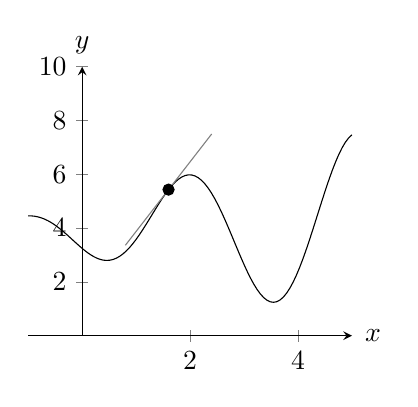
\begin{tikzpicture}
			\begin{axis}[
				scale = 0.6,
				axis x line = middle,
				axis y line = middle,
				xmin = -1,
				xmax = 5,
				ymin = 0,
				ymax = 10,
				xlabel = $x$,
				ylabel = $y$,
				every axis x label/.style = {
					at = {(ticklabel* cs:1.01)},
					anchor = west,
				},
				every axis y label/.style = {
					at = {(ticklabel* cs:1.01)},
					anchor = south,
				},
				]
				\addplot[
				black,
				samples = 100,
				domain = -1:5,
				]{0.5*(x+2)*sin((2*(x+2))r)+4};
				\addplot[
				gray,
				samples = 10,
				domain = 0.8:2.4
				]{2.5869*x + 1.28956};
				\addplot[mark=*] coordinates {(1.6, 5.4286)};
			\end{axis}
		\end{tikzpicture}
		\caption{Plot of a less straight line.}
		\label{lec3:notstraight}
	\end{subfigure}
	\caption{Examples of tangents of functions.}
\end{figure}

\noindent
If the function at hand is a (nonvertical) straight line, this is simple.
We read of a coefficient, or we compute rise over run, et cetera.

If, on the other hand, the function isn't a straight line, it can be slightly more complicated.
To do it, we simply fall back on what is essentially basic geometry in order to attempt to approximate the tangent line of the function at the point of interest.
We demonstrate by drawing on Figure \ref{lec3:notstraight} above, attempting to find the slope at $x = a$.

\begin{figure}
	\centering
	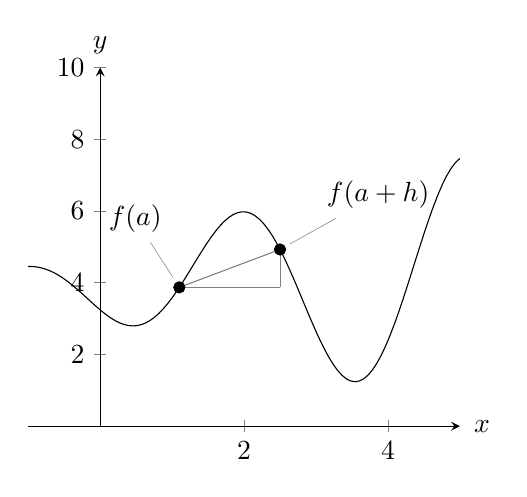
\begin{tikzpicture}
		\begin{axis}[
			scale = 0.8,
			axis x line = middle,
			axis y line = middle,
			xmin = -1,
			xmax = 5,
			ymin = 0,
			ymax = 10,
			xlabel = $x$,
			ylabel = $y$,
			every axis x label/.style = {
				at = {(ticklabel* cs:1.01)},
				anchor = west,
			},
			every axis y label/.style = {
				at = {(ticklabel* cs:1.01)},
				anchor = south,
			},
			]
			\addplot[
			black,
			samples = 100,
			domain = -1:5,
			]{0.5*(x+2)*sin((2*(x+2))r)+4};
			\addplot[
			gray,
			solid
			] coordinates {(1.1, 3.87121) (2.5, 4.92727)};
			\addplot[
			gray,
			solid
			] coordinates {(2.5, 4.92727) (2.5, 3.87121)};
			\addplot[
			gray,
			solid
			] coordinates {(2.5, 3.87121) (1.1, 3.87121)};
			\addplot[mark=*] coordinates {(1.1, 3.87121)} node[pin=100:{$f(a)$}]{} ;
			\addplot[mark=*] coordinates {(2.5, 4.92727)} node[pin=40:{$f(a + h)$}]{} ;
		\end{axis}
	\end{tikzpicture}
	\hfill
	\begin{tikzpicture}
		\draw[white] (1, 1.6);
		\draw (1.1, 3.87121) -- (3.5, 4.92727) -- node[right] {$f(a + h) - f(a)$} (3.5, 3.87121) -- node[below] {$a + h - a$} cycle;
		\draw (3.3, 3.87121) -- (3.3, 4.07121) -- (3.5, 4.07121);
	\end{tikzpicture}
	\caption{Constructing a difference quotient.}
\end{figure}

In other words, we let the point $(a, f(a))$ that we are interested in be one of the corners of a triangle, and pick some real number $h$ to construct another point $(a + h, f(a + h))$ on the curve.

As illustrated below, that creates a right triangle with base $a + h - a = h$ and height $f(a + h) - f(a)$. Hence to find the slope of the hypotenuse, we compute the rise over the run and arrive at
\[
	\text{slope} = \frac{\text{rise}}{\text{run}} = \frac{f(a + h) - f(a)}{h}
\]
of the line we just constructed.
The expression in the right-hand side is called a \keyword{difference quotient}\index{difference quotient}, or sometimes a \keyword{Newton quotient}\index{Newton quotient|see {difference quotient}}.

The trick is to now let $h$ go to $0$, but never quite reach it.
That way we will approach the slope at $x = a$, which is all right, because we know limits!

\topic{Definition and Computaitonal Rules}

Having done this we are ready to formalise the definition of the derivative.

\begin{definition}[Derivative, differentiability]
	The \keyword{derivative}\index{derivative} of a function $f$ is another function $f'$ defined by
	\[
		f'(x) = \lim_{h \to 0} \frac{f(x + h) - f(x)}{h}
	\]
	at all points $x$ for which the limit exists (in the sense that it is finite (and real, in this course)).

	If $f'(x)$ exists (at a given $x$), we say that $f$ is \keyword{differentiable}\index{differentiability} at $x$.
\end{definition}

\begin{remark}\label{lec3:singularpoint}
	The domain of $f'$ may be smaller than the domain of $f$, since $f$ need not be differentiable everywhere.
	Points where $f$ is not differentiable (and that aren't endpoints of closed intervals in the domain) are called \keyword{singular points}\index{singular point}.

	Moreover, note that the limit in the definition prevents a function from being differentiable at an isolated point.
	That is to say, for a function to be differentiable at a point, it must also be defined at some neighbourhood around that point.
\end{remark}

\begin{remark}
	An equivalent difference quotient limit that some people prefer is
	\[
		\lim_{x \to x_0} \frac{f(x) - f(x_0)}{x - x_0}.
	\]

	\noindent
	To see that this accomplishes the same thing, try drawing the corresponding picture.
\end{remark}

\begin{example}
	By definition, $f'(x)$ is the slope of $y = f(x)$ at the point $x = x_0$, where it exists.
	Therefore the tangent line to $y = f(x)$ at $(x_0, f(x_0))$ is
	\[
		y = f(x_0) + f'(x_0) (x - x_0). \qedhere
	\]
\end{example}

\noindent
It should be noted that the derivative comes with many different notations.
If our function is $y = f(x)$, the following all mean the same thing:
\[
	D_x y = y' = \frac{d y}{d x} = \frac{d}{d x} f = f' = D_x f = D f.
\]
In some of these, the variable $x$ is implied, whereas in others it is explicit.
For us, doing calculus in only one variable, there will probably never be any ambiguity in not specifying the variable, but once one starts doing calculus in more variables, it becomes a very good idea to specify.

Finally, before we go on to prove various interesting properties of the derivative, we make a note about what happens at endpoints of closed intervals in the domains of functions, thereby also clarifying what we meant by the parentheses in Remark \ref{lec3:singularpoint} above.

\begin{remark}[Left and right derivatives]
	Suppose our function $f$ that we wish to differentiate is defined on a closed interval $\interval{a}{b}$.
	We have a problem if we try to compute $f'(a)$ or $f'(b)$.

	Consider, for instance, $x = a$.
	What happens if $h < 0$ in the difference quotient?
	Well, in $f(a + h)$ we have $x = a + h < a$, and for such a value of $x$ the function $f$ isn't defined.

	The solution is to use one-sided limits where appropriate, to define \keyword{left} and \keyword{right derivatives}\index{derivative!left}\index{derivative!right}:
	\[
		f'_+(a) = \lim_{h \to 0^+} \frac{f(a + h) - f(a)}{h} \qquad \text{and} \qquad f'_- (b) = \lim_{h \to 0^-} \frac{f(b + h) - f(b)}{h}.
	\]
\end{remark}

\noindent
There is an important connection between differentiability and continuity.

\begin{theorem}\label{lec3:diffimpliescont}
	If $f$ is differentiable at $x$, then it is also continuous at $x$.
\end{theorem}

\begin{proof}
	Since $f$ is differentiable at $x$, the limit
	\[
		f'(x) = \lim_{h \to 0} \frac{f(x + h) - f(x)}{h}
	\]
	exists. We then take the difference between $\lim\limits_{h \to 0} f(x + h)$ and $f(x)$:
	\begin{align*}
		\lim\limits_{h \to 0} (f(x + h)) - f(x) & = \lim_{h \to 0} (f(x + h) - f(x)) = \lim_{h \to 0} \frac{f(x + h) - f(x)}{h} \cdot h  \\
		                                        & = \lim_{h \to 0} \frac{f(x + h) - f(x)}{h} \cdot \lim_{h \to 0} h = f'(x) \cdot 0 = 0.
	\end{align*}
	This means that the distance between the limit of $f$ at $x$ and $f(x)$ is 0, whereby they are equal, so by definition $f$ is continuous at $x$.
\end{proof}

\noindent
The converse is not true, i.e. there exists continuous functions that aren't differentiable.

\begin{counterexample}
	Consider the absolute value function $f(x) = \abs{x}$.
	This function is continuous at the point $x = 0$ ($\delta = \varepsilon$ works fine in the definition of continuity, for instance), but it is not differentiable there, since the the limit defining the derivative doesn't exist there; from the left the limit is $-1$, whereas from the right the limit is $1$.
\end{counterexample}

\noindent
We now formulate and prove various computational rules of derivatives that we will continue using throughout the course.

\begin{theorem}[Addition, subtraction, and multiplication by constant]
	Let $f$ and $g$ be differentiable functions at $x$, and let $k$ be some constant.
	Then $f + g$, $f - g$, and $k f$ are all differentiable at $x$, and
	\begin{romanlist}
		\item $(f + g)'(x) = f'(x) + g'(x)$;
		\item $(f - g)'(x) = f'(x) - g'(x)$; and
		\item $(k f)'(x) = k f'(x)$.
	\end{romanlist}
\end{theorem}

\begin{proof}
	We simply rearrange the difference quotients and use our rules for limits.
	For \fakeitemref{1} and \fakeitemref{2}, this becomes
	\begin{align*}
		(f \pm g)'(x) & = \lim_{h \to 0} \frac{(f \pm g)(x + h) - (f \pm g)(x)}{h}                                                   \\
		              & = \lim_{h \to 0} \frac{f(x + h) \pm g(x + h) - (f(x) \pm g(x))}{h}                                           \\
		              & = \lim_{h \to 0} \frac{f(x + h) - f(x)}{h} \pm \lim_{h \to 0} \frac{(g(x + h) - g(x))}{h} = f'(x) \pm g'(x).
	\end{align*}

	\noindent
	For \fakeitemref{3}, we get a similarly trivial computation:
	\[
		(k f)'(x) = \lim_{h \to 0} \frac{k f(x + h) - k f(x)}{h} = k \cdot \lim_{h \to 0} \frac{f(x + h) - f(x)}{h} = k f'(x). \qedhere
	\]
\end{proof}

\noindent
What happens when multiplying two functions together is perhaps less intuitive:

\begin{theorem}[Product rule]
	Let $f$ and $g$ be functions differentiable at $x$.
	Then $f g$ is also differentiable at $x$, and
	\[
		(f g)'(x) = f'(x) g(x) + f(x) g'(x).
	\]
\end{theorem}

\begin{proof}
	We study the difference quotient and add $0$ in a clever way:
	\begin{align*}
		(f g)'(x) & = \lim_{h \to 0} \frac{f(x + h) g(x + h) - f(x) g(x)}{h}                                                         \\
		          & = \lim_{h \to 0} \frac{f(x + h) g(x + h) - f(x) g(x + h) + f(x) g(x + h) - f(x) g(x)}{h}                         \\
		          & = \lim_{h \to 0} \Big ( \frac{f(x + h) - f(x)}{h} \cdot g(x + h) + f(x) \cdot \frac{g(x + h) - g(x)}{h} \Big )   \\
		          & = \lim_{h \to 0} \frac{f(x + h) - f(x)}{h} \cdot g(x + h) + \lim_{h \to 0} f(x) \cdot \frac{g(x + h) - g(x)}{h}  \\
		          & = \lim_{h \to 0} \frac{f(x + h) - f(x)}{h} \cdot g(x + h) + f(x) \cdot \lim_{h \to 0} \frac{g(x + h) - g(x)}{h}.
	\end{align*}
	The crucial last step is to now recall Theorem \ref{lec3:diffimpliescont}, whereby $g$ is continuous, and therefore the above becomes
	\[
		(f g)'(x) = f'(x) g(x) + f(x) g'(x). \qedhere
	\]
\end{proof}

\noindent
Dealing with quotients is maybe even less intuitive.

\begin{theorem}[Quotient rule]
	If $f$ and $g$ are differentiable functions at $x$ and $g(x) \neq 0$, then the quotient $f / g$ is differentiable at $x$, and
	\[
		\Big ( \frac{f}{g} \Big )'(x) = \frac{f'(x) g(x) - f(x) g'(x)}{(g(x))^2}.
	\]
\end{theorem}

\noindent
To prove it, we first prove an easier result.

\begin{lemma}[Reciprocal rule]
	If $g$ is differentiable at $x$ with $g(x) \neq 0$, then $1 / g$ is differentiable at $x$ and
	\[
		\Big ( \frac{1}{g} \Big )'(x) = -\frac{g'(x)}{(g(x))^2}.
	\]
\end{lemma}

\begin{proof}
	The trick lies entirely in writing the numerator with common denominator:
	\begin{align*}
		\frac{d}{d x} \Big ( \frac{1}{g(x)} \Big ) & = \lim_{h \to 0} \frac{\frac{1}{g(x + h)} - \frac{1}{g(x)}}{h} = \lim_{h \to 0} \frac{\frac{g(x) - g(x + h)}{g(x + h) g(x)}}{h} \\
		                                           & = \lim_{h \to 0} \frac{g(x) - g(x + h)}{h g(x + h) g(x)} = - \lim_{h \to 0} \frac{g(x + h) - g(x)}{h g(x + h) g(x)}             \\
		                                           & = - \lim_{h \to 0} \frac{1}{g(x) g(x + h)} \cdot \frac{g(x + h) - g(x)}{h}                                                      \\
		                                           & = - \frac{g'(x)}{(g(x))^2}. \qedhere
	\end{align*}
\end{proof}

\noindent
With this at our disposal proving the quotient rule becomes a special case of the product rule.

\begin{proof}[Proof of the Quotient rule]
	We write $f / g$ as $f \cdot 1 / g$ and use the product rule:
	\begin{align*}
		\frac{d}{d x} \Big ( \frac{f(x)}{g(x)} \Big ) & = \frac{d}{d x} \Big ( f(x) \cdot \frac{1}{g(x)} \Big ) = f'(x) \frac{1}{g(x)} + f(x) \Big ( \frac{- g'(x)}{(g(x))^2} \Big ) \\
		                                              & = \frac{f'(x) g(x) - f(x) g'(x)}{(g(x))^2}. \qedhere
	\end{align*}
\end{proof}

\noindent
In keeping with how we dealt with continuity, after addition, subtraction, multiplication and division comes composition.

\begin{theorem}[Chain rule]
	If $f$ is differentiable at $y = g(x)$, and $g$ is differentiable at $x$, then $f \circ g$ is differentiable at $x$ and $(f \circ g)'(x) = f'(g(x)) g'(x)$.
\end{theorem}

\begin{proof}
	We construct a slightly tricky function $E$, defined as
	\[
		E(k) = \begin{cases}
		0, & \text{if}~ k = 0 \\
		\frac{f(y + k) - f(y)}{k} - f'(y), & \text{if}~ k \neq 0.
		\end{cases}
	\]
	Notice how
	\[
		\lim_{k \to 0} E(k) = \lim_{k \to 0} \frac{f(y + k) - f(y)}{k} - \lim_{k \to 0} f'(y) = f'(y) - f'(y) = 0 = E(0),
	\]
	meaning that $E(k)$ is continuous at $k = 0$.
	Moreover
	\[
		E(k) + f'(y) = \frac{f(y + k) - f(y)}{k},
	\]
	which implies that
	\[
		f(y + k) - f(y) = (E(k) + f'(y)) \cdot k.
	\]

	\noindent
	If we now take $y = g(x)$ and $k = g(x + h) - g(x)$, meaning that $y + k = g(x + h)$, and inserting this into the above equation we get
	\begin{equation}\label{lec3:chaindiff}
		f(g(x + h)) - f(g(x)) = \big (f'(g(x)) + E(k) \big ) (g(x + h) - g(x)).
	\end{equation}

	\noindent
	By assumption $g$ is differentiable at $x$, meaning that
	\[
		g'(x) = \lim_{h \to 0} \frac{g(x + h) - g(x)}{h},
	\]
	and also that $g$ is continuous at $x$, whereby $\lim\limits_{h \to 0} g(x + h) - g(x) = 0$.

	We are now ready to compute the limit of the difference quotient of the composition, using Equation \ref{lec3:chaindiff} straight away:
	\[
		\frac{d}{d x} f(g(x)) = \lim_{h \to 0} \frac{f(g(x + h)) - f(g(x))}{h} = \lim_{h \to 0} (f'(g(x)) + E(k)) \, \frac{g(x + h) - g(x)}{h}.
	\]
	Now since $E$ is continuous at $0 = \lim\limits_{h \to 0} g(x + h) - g(x) = \lim\limits_{h \to 0} k$, we have
	\[
		\lim_{h \to 0} E(k) = E \Big ( \lim_{h \to 0} k \Big ) = E(0) = 0,
	\]
	whereby the above becomes
	\[
		\frac{d}{d x} f(g(x)) = f'(g(x)) g'(x). \qedhere
	\]
\end{proof}

\topic{Derivatives of Trigonometric Functions}

We state without proof that $\sin$ and $\cos$ are continuous functions everywhere.

Moreover, we claim that $\lim\limits_{x \to 0} \sin(x) = 0$ and $\lim\limits_{x \to 0} \cos(x) = 1$.

\begin{exercise}
	Try to prove it.

	\emph{Hint: for the first one, use $\sin(\alpha + \beta) - \sin(\alpha - \beta) = 2 \cos(\alpha)\sin(\beta)$ to manipulate $\abs{\sin(x) - \sin(a)}$ into a single $\sin$.
	For both this and the $\sin$ limit, it will help to prove that $0 \leq \abs{\sin(x)} \leq \abs{x}$.}
\end{exercise}

\noindent
In closing, we will prove an important limit, which we will use next time to compute the derivatives of $\sin$ and $\cos$.

\begin{lemma}
	$\displaystyle \lim_{x \to 0} \frac{\sin(x)}{x} = 1$.
\end{lemma}

\begin{proof}
	This proof relies very much on the geometrical construction of $\sin$ and $\tan$ found in Figure \ref{lec3:sinx/x}.
	Let $0 < x < \pi / 2$.

	\begin{figure}[t]
		\centering
		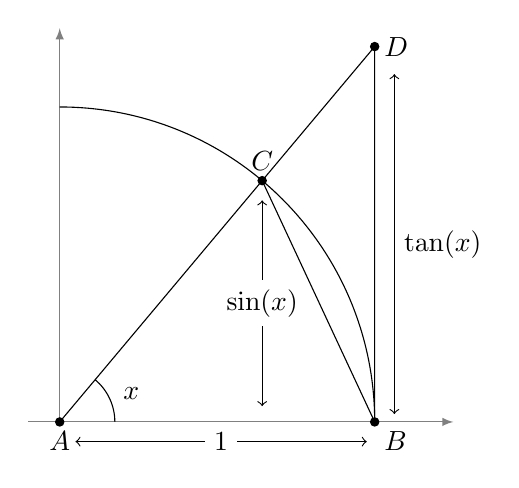
\begin{tikzpicture}[scale = 1]

			\draw[gray,-latex](-0.4, 0) -- (5, 0); % x-axis
			\draw[gray,-latex](0, -0.4) -- (0, 5); % y-axis
			\pic{circle arc = 0:90:4}; % Unit circle

			\draw (0, 0) node[below, fill = white]{$A$} coordinate (A);
			\filldraw (A) circle[radius = 1.5pt];

			\draw (4, 0) node[below right]{$B$} coordinate (B);
			\filldraw (B) circle[radius = 1.5pt];

			\draw (50:4) node[above]{$C$} coordinate (C);
			\filldraw (C) circle[radius = 1.5pt];

			\draw (4, 4.767) node[right]{$D$} coordinate (D);
			\filldraw (D) circle[radius = 1.5pt];

			\draw[black] (A) -- (D) -- (B) -- (C);
			\draw[<->] (0.2, -0.25) -- node[midway, fill = white]{$1$} (3.9, -0.25);
			\draw[<->] (4.25, 0.1) -- node[midway, right, fill = white]{$\tan(x)$} (4.25, 4.417);
			\draw[<->] (2.571, 0.2) -- node[midway, fill = white]{$\sin(x)$} (2.571, 2.814);

			\pic[draw, angle eccentricity=1.2, angle radius = 0.7cm, "$\quad\!x$"]{angle=B--A--D};
		\end{tikzpicture}
		\caption{A geometrical representation of $\sin$ and $\tan$ on the unit circle.}
		\label{lec3:sinx/x}
	\end{figure}

	We make three claims:
	\begin{romanlist}
		\item The area of the triangle $\triangle A B C$ is $\frac{1}{2} \sin(x)$ (since $\sin(x)$ is its height).
		\item The area of the sector $A B C$ is $\frac{1}{2} x$.
		\item The area of the triangle $\triangle A B D$ is $\frac{1}{2} \tan(x)$.
	\end{romanlist}

	\noindent
	Moreover, it is clear that these areas are in ascending order as listed, i.e.
	\[
		\frac{1}{2} \sin(x) \leq \frac{1}{2} x \leq \frac{1}{2} \tan(x).
	\]
	If we divide by $\frac{1}{2} \sin(x)$, which is positive since $0 < x < \pi / 2$, we then get
	\[
		1 \leq \frac{x}{\sin(x)} \leq \frac{1}{\cos(x)}.
	\]
	Finally we take reciprocals, thereby reversing the inequalities,
	\[
		\cos(x) \leq \frac{\sin(x)}{x} \leq 1.
	\]

	\noindent
	Note how $1$, $\sin(x) / x$, and $\cos(x)$ are all even functions, so this chain of inequalities is true also for $-\pi / 2 < x < 0$ by symmetry.
	This is good, because it allows us to consider the two-sided limit we are interested in, despite the geometric picture only discussing positive $x$.

	Finally we remark that since $\lim\limits_{x \to 0} \cos(x) = 1$, the Squeeze theorem tells us that
	\[
		\lim_{x \to 0} \frac{\sin(x)}{x} = 1,
	\]
	as desired.
\end{proof}


\lecture[January 30, 2017]{The Mean-Value Theorem}

%!TEX root = ../lectures.tex

\topic{Trigonometric Derivatives, continued}

Recall from last time how
\[
	\lim_{x \to 0} \frac{\sin(x)}{x} = 1.
\]

\noindent
Using this we can prove

\begin{proposition}
	$\displaystyle \frac{d}{d x} \sin(x) = \cos(x)$.
\end{proposition}

\begin{proof}
	We need the identity $\sin(\alpha + \beta) = \sin(\alpha) \cos(\beta) + \cos(\alpha) \sin(\beta)$.
	Then
	\begin{align*}
		\frac{d}{d x} \sin(x) & = \lim_{h \to 0} \frac{\sin(x + h) - \sin(x)}{h}                                                                                                                                             \\
		                      & = \lim_{h \to 0} \frac{\sin(x) \cos(h) + \cos(x) \sin(h) - \sin(x)}{h}                                                                                                                       \\
		                      & = \lim_{h \to 0} \frac{\sin(x) (\cos(h) - 1) + \cos(x) \sin(h)}{h}                                                                                                                           \\
		                      & = \Big ( \lim_{h \to 0} \sin(x) \Big ) \cdot \Big ( \lim_{h \to 0} \frac{\cos(h) - 1)}{h} \Big ) + \Big ( \lim_{h \to 0} \cos(x) \Big ) \cdot \Big ( \lim_{h \to 0} \frac{\sin(h)}{h} \Big ) \\
		                      & = \sin(x) \cdot 0 + \cos(x) \cdot 1 = \cos(x).
	\end{align*}

	\noindent
	The only mystery in the above computation is the $\cos(h)$ limit in the penultimate line.
	We shed light on it by using $\cos(h) = 1 - 2 (\sin(h / 2))^2$, like so
	\[
		\lim_{h \to 0} \frac{\cos(h) - 1}{h} = - \lim_{h \to 0} \frac{2 (\sin(h / 2))^2}{h},
	\]
	which if we let $x = h / 2$ (which also approaches $0$ as $h$ does) becomes
	\[
		- \lim_{x \to 0} \frac{\sin(x)}{x} \cdot \sin(x) = -1 \cdot 0 = 0. \qedhere
	\]
\end{proof}

\noindent
Since we have a chain rule, it is immediate to find the derivative of $\cos$ once we know the derivative of $\sin$.

\begin{corollary}
	$\displaystyle \frac{d}{d x} \cos(x) = - \sin(x)$.
\end{corollary}

\begin{proof}
	We know that $\cos(x) = \sin(\pi/2 - x)$, and $\sin(x) = \cos(\pi/2 - x)$, whence by the chain rule
	\begin{align*}
		\frac{d}{d x} \cos(x) & = \frac{d}{d x} \sin\Big ( \frac{\pi}{2} - x \Big ) = \cos \Big ( \frac{\pi}{2} - x \Big ) \cdot \frac{d}{d x} \Big ( \frac{\pi}{2} - x \Big ) \\
		                      & = - \cos \Big ( \frac{\pi}{2} - x \Big ) = - \sin(x). \qedhere
	\end{align*}
\end{proof}

\begin{exercise}
	Use the computational rules to find the derivatives of $\tan$, $\sec$, $\cot$, and $\csc$, in the event that you like these functions.
\end{exercise}

\noindent
Since so far the discussion about derivatives has been quite heavy on theory, we close it off with a number of computational problems, so as to hopefully get some practice with how the definition of the derivative works. In the future we will often end up computing derivatives directly using results such as these, instead of falling back on the definition in terms of the limit of a difference quotient.

\begin{exercises}
Show the following:
\begin{alphalist}
	\item $\displaystyle \frac{d}{d x} c = 0$, where $c$ is constant.
	\item $\displaystyle \frac{d}{d x} k x = k$, where $k$ is constant.
	\item $\displaystyle \frac{d}{d x} \frac{1}{x} = - \frac{1}{x^2}$.
	\item $\displaystyle \frac{d}{d x} \sqrt{x} = \frac{1}{2 \sqrt{x}}$.
	\item $\displaystyle \frac{d}{d x} x^n = n x^{n - 1}$, for all $n \in \Z$, perhaps using induction.
\end{alphalist}
\end{exercises}

\noindent
Note how, for instance, \fakeitemref{a}, \fakeitemref{b}, and \fakeitemref{e} combined, together with our computational rules, tell us how to differentiate every possible polynomial.

The majority of this lecture will be about the Mean-value theorem and some consequences thereof, but first we will wrap up the discussion of the derivative itself somewhat.

\topic{Higher Order Derivatives}

Since, by definition, the derivative of a function $y = f(x)$ is again a function, it can happen that the derivative itself is differentiable (at some point(s)).

We call this derivative of a derivative the \keyword{second derivative}\index{derivative!higher order}\index{derivative!second} of the original function.
Like the first derivative, there are many notations used for this:
\[
	y'' = f'' = \frac{d^2 y}{d x^2} = \frac{d}{d x} \frac{d}{d x} f = \frac{d^2}{d x^2} f = D_x^2 y = D_x^2 f.
\]

\noindent
We can continue this to achieve a general $n$th order derivative,
\[
	y^{(n)} = f^{(n)} = \frac{d^n y}{d x^n} = \frac{d^n}{d x^n} f = D_x^n y = D_x^n f,
\]
defined inductively as the derivative of the $(n - 1)$st order derivative.

\begin{remark}
	We use $y^{(n)}$ or $f^{(n)}$, with the parentheses, in order to distinguish higher order derivatives from exponents or compositions,
	\[
		y^n = \underbrace{y \cdot y \cdot \ldots \cdot y}_{n ~\text{lots of}~ y}, \qquad \text{or} \qquad  f^n = \underbrace{f \circ f \circ \cdots \circ f}_{n~\text{lots of}~f}.
	\]
\end{remark}

\noindent
For convenience the function itself is usually taken to be its own zeroth derivative, $f = f^{(0)}$.

\begin{example}
	The classical example is the reason calculus was invented: take $x = x(t)$ to be the position (of something) at the time $t$.
	Then its velocity is $v = \frac{d x}{d t} = x'$, and its acceleration is $a = \frac{d v}{d t} = \frac{d^2 x}{d t^2} = x''$.
	This exemplifies why we often want to think of the derivative as the rate of change of something.
\end{example}

\noindent
These higher order derivatives are often very important in physics, since it turns out that much in the real world can be modeled using so-called differential equations, which we will deal more with toward the end of the course.
For now, we'll discuss it briefly in an example.

\begin{example}
	Show that $y(t) = A \cos(k t) + B \sin(k t)$, for $A$, $B$, and $k$ constants, is a solution to the \keyword{second-order differential equation}\index{differential equation}\index{differential equation!second order}
	\[
		\frac{d^2 y}{d t^2} (t) + k^2 y(t) = 0.
	\]
	To do this we compute the second derivative and test it in the equation (when we deal with differential equations more thoroughly in the future we will learn how to find these solutions on our own):
	\[
		\frac{d^2 y}{d t^2}(t) = \frac{d}{d t} (-A k \sin(k t) + B k \cos(k t)) = -A k^2 \cos(k t) - B k^2 \sin(k t).
	\]
	We then insert it into the differential equation,
	\[
		\frac{d^2 y}{d t^2} (t) + k^2 y(t) = - k^2 (A \cos(k t) + B \sin(k t)) + k^2 (A \cos(k t) + B \sin(k t)) = 0
	\]
	for all $t$.
\end{example}

\topic{The Mean-Value Theorem}

\begin{example}
	Suppose we leave on a trip at 3 o'clock, traveling 100 kilometres away, and arriving 2 hours later, at 5 o'clock.
	Then of course our average speed was
	\[
		\frac{\SI{100}{\kilo\metre}}{\SI{2}{\hour}} = \SI[per-mode = symbol]{50}{\kilo\metre\per\hour}.
	\]
	We might not have traveled at this speed constantly (indeed it's unlikely we did, since we presumably started at rest and accelerated), but we \emph{must} have traveled at $\SI[per-mode = symbol]{50}{\kilo\metre\per\hour}$ at least once!

	If not, our speed was either always above or always below $\SI[per-mode = symbol]{50}{\kilo\metre\per\hour}$, in which case we would have arrived either before or after 5 o'clock.
\end{example}

\noindent
In the language of calculus, this is called the Mean-value theorem, and the crucial detail that makes it true is, of course, that our speed whilst traveling can't `jump'.
I.e., we can't go from $\SI[per-mode = symbol]{25}{\kilo\metre\per\hour}$ to $\SI[per-mode = symbol]{75}{\kilo\metre\per\hour}$ without ever passing $\SI[per-mode = symbol]{50}{\kilo\metre\per\hour}$.
Once again in the language of calculus, this is what we call continuity, and indeed since we have acceleration of some kind everywhere, even if constant, our speed (or velocity) must also have a derivative.

\begin{theorem}[Mean-value theorem]\index{mean-value theorem}
	Let $f$ be a function continuous on the closed and finite interval $\interval{a}{b}$ that is differentiable on $\interval[open]{a}{b}$.
	Then there exists a point $c \in \interval[open]{a}{b}$ such that
	\[
		\frac{f(b) - f(a)}{b - a} = f'(c).
	\]
\end{theorem}

\begin{figure}
	\centering
	\begin{tikzpicture}
		\begin{axis}[
			scale = 0.8,
			axis x line = left,
			axis y line = left,
			xmin = -1,
			xmax = 5,
			ymin = 0,
			ymax = 10,
			xlabel = $x$,
			ylabel = $y$,
			xtick = {0.5, 4.5},
			xticklabels = {$a$, $b$},
			ytick = {4.80134, 7.36554},
			yticklabels = {$f(a)$, $f(b)$},
			every axis x label/.style = {
				at = {(ticklabel* cs:1.01)},
				anchor = west,
			},
			every axis y label/.style = {
				at = {(ticklabel* cs:1.01)},
				anchor = south,
			},
			]
			\addplot[
			black,
			samples = 100,
			domain = 0.5:4.5,
			]{0.5*(x+2)*sin((2*(x+2))r)+6};
			\addplot[
			gray,
			dashed
			] coordinates {(0.5, 1.29134) (4.5, 3.85554)};
			\addplot[
			gray,
			dashed
			] coordinates {(0.5, 7.05234) (4.5, 9.61654)};
			\addplot[
			gray,
			dashed
			] coordinates {(0.5, 4.80134) (4.5, 7.36554)};
			\addplot[mark=*] coordinates {(0.5, 4.80134)};
			\addplot[mark=*] coordinates {(4.5, 7.36554)};
			\addplot[mark=*] coordinates {(1.90890, 7.95317)};
			\addplot[mark=*] coordinates {(3.59946, 3.25795)};
		\end{axis}
	\end{tikzpicture}
	\caption{Illustration of the Mean-value theorem.}
	\label{lec4:meanval}
\end{figure}


\noindent
That is to say, there must exist some point(s) in the interior of the interval with the same slope as the line segment connecting the two endpoints.

An example of this theorem is demonstrated in Figure \ref{lec4:meanval}, which also demonstrates that the $c$ in the theorem needn't be unique.
We will prove this in a bit, but for now we will establish some more theory and also motivate why both the continuity and the differentiability is required in Figure \ref{lec4:meanvalcounter}.

\begin{figure}
	\centering
	\begin{subfigure}{0.3\textwidth}
		\centering
		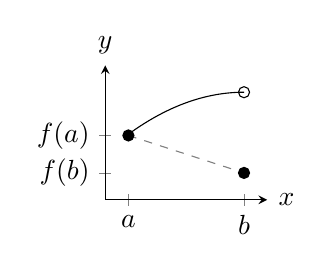
\begin{tikzpicture}
			\begin{axis}[
				scale = 0.3,
				axis x line = left,
				axis y line = left,
				xmin = 0,
				xmax = 3.5,
				ymin = 0,
				ymax = 10,
				xlabel = $x$,
				ylabel = $y$,
				xtick = {0.5, 3},
				xticklabels = {$a$, $b$},
				ytick = {4.785, 2},
				yticklabels = {$f(a)$, $f(b)$},
				every axis x label/.style = {
					at = {(ticklabel* cs:1.01)},
					anchor = west,
				},
				every axis y label/.style = {
					at = {(ticklabel* cs:1.01)},
					anchor = south,
				},
				]
				\addplot[
				black,
				samples = 100,
				domain = 0.5:3,
				]{-0.5*(x-3)^2+8};
				\addplot[
				gray,
				dashed
				] coordinates {(0.5, 4.785) (3, 2)};
				\addplot[mark=*] coordinates {(0.5, 4.785)};
				\addplot[mark=o] coordinates {(3, 8)};
				\addplot[mark=*] coordinates {(3, 2)};
			\end{axis}
		\end{tikzpicture}
		\caption{Discontinuous at endpoint}
	\end{subfigure}
	\quad
	\begin{subfigure}{0.3\textwidth}
		\centering
		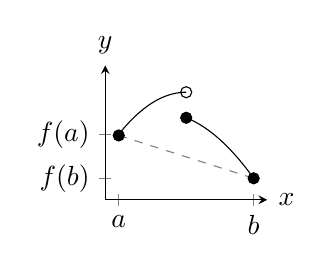
\begin{tikzpicture}
			\begin{axis}[
				scale = 0.3,
				axis x line = left,
				axis y line = left,
				xmin = 0,
				xmax = 6,
				ymin = 0,
				ymax = 10,
				xlabel = $x$,
				ylabel = $y$,
				xtick = {0.5, 5.5},
				xticklabels = {$a$, $b$},
				ytick = {4.875, 1.6},
				yticklabels = {$f(a)$, $f(b)$},
				every axis x label/.style = {
					at = {(ticklabel* cs:1.01)},
					anchor = west,
				},
				every axis y label/.style = {
					at = {(ticklabel* cs:1.01)},
					anchor = south,
				},
				]
				\addplot[
				black,
				samples = 100,
				domain = 0.5:3,
				]{-0.5*(x-3)^2+8};
				\addplot[
				black,
				samples = 100,
				domain = 3:5.5,
				]{-0.4*(x-2)^2+6.5};
				\addplot[
				gray,
				dashed
				] coordinates {(0.5, 4.785) (5.5, 1.6)};
				\addplot[mark=*] coordinates {(0.5, 4.785)};
				\addplot[mark=o] coordinates {(3, 8)};
				\addplot[mark=*] coordinates {(3, 6.1)};
				\addplot[mark=*] coordinates {(5.5, 1.6)};
			\end{axis}
		\end{tikzpicture}
		\caption{Discontinuous at interior point}
	\end{subfigure}
	\quad
	\begin{subfigure}{0.3\textwidth}
		\centering
		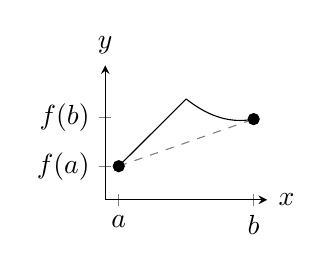
\begin{tikzpicture}
			\begin{axis}[
				scale = 0.3,
				axis x line = left,
				axis y line = left,
				xmin = 0,
				xmax = 6,
				ymin = 0,
				ymax = 10,
				xlabel = $x$,
				ylabel = $y$,
				xtick = {0.5, 5.5},
				xticklabels = {$a$, $b$},
				ytick = {2.5, 6.1},
				yticklabels = {$f(a)$, $f(b)$},
				every axis x label/.style = {
					at = {(ticklabel* cs:1.01)},
					anchor = west,
				},
				every axis y label/.style = {
					at = {(ticklabel* cs:1.01)},
					anchor = south,
				},
				]
				\addplot[
				black,
				samples = 100,
				domain = 0.5:3,
				]{2*x+1.5};
				\addplot[
				black,
				samples = 100,
				domain = 3:5.5,
				]{0.4*(x-5)^2+5.9};
				\addplot[
				gray,
				dashed
				] coordinates {(0.5, 2.5) (5.5, 6)};
				\addplot[mark=*] coordinates {(0.5, 2.5)};
				\addplot[mark=*] coordinates {(5.5, 6)};
			\end{axis}
		\end{tikzpicture}
		\caption{Not differentiable at interior point}
	\end{subfigure}
	\caption{Counterexamples of the Mean-value theorem where essential conditions are violated.}
	\label{lec4:meanvalcounter}
\end{figure}


This demonstrates that if we lack continuity anywhere in the closed interval, then we can construct a counter example, and likewise if we lack differentiability anywhere in the open interval, we may do the same.

We now prove an intermediary result we need in order to prove the Mean-value theorem.

\begin{lemma}\label{lec4:criticalpoint}
	If $f$ is defined on an open interval $\interval[open]{a}{b}$ and achieves a maximum (or minimum) at $c \in \interval[open]{a}{b}$, then if $f'(c)$ exists, it must be $0$.
\end{lemma}

\noindent
Such points where the derivative is $0$ are called \keyword{critical points}\index{critical point}.

\begin{proof}
	If $f$ has a maximum at $c \in \interval[open]{a}{b}$, then $f(x) - f(c) \leq 0$ for all $x \in \interval[open]{a}{b}$.
	We consider two cases:

	\fakeitem{1} If $c < x < b$, then
	\[
		\frac{f(x) - f(c)}{x - c} \leq 0,
	\]
	since $c < x$, which, if we recall the alternative difference quotient,\footnote{It is of course possible to compute the same with the $h \to 0$ type difference quotient, it's just marginally more cumbersome.} implies the sign of the right derivative at $c$,
	\[
		f'_+(c) = \lim_{x \to c} \frac{f(x) - f(c)}{x - c} \leq 0.
	\]

	\noindent
	\fakeitem{2} Similarly if $a < x < c$, then we have
	\[
		\frac{f(x) - f(c)}{x - c} \geq 0
	\]
	which similarly implies
	\[
		f'_-(c) = \lim_{x \to c} \frac{f(x) - f(c)}{x - c} \geq 0.
	\]

	\noindent
	By assumption $f'(c)$ exists, so it is equal to the left and right derivative at that point, so
	\[
		0 \leq f'_-(c) = f'(c) = f'_+(c) \leq 0,
	\]
	whereby $f'(c) = 0$.

	For the case of the minimum, the proof is almost identical, except we change the direction of certain inequalities.
\end{proof}

\noindent
We now show a special case of the Mean-value theorem, with which we later prove the full version.

\begin{theorem}[Rolle's theorem]\index{Rolle's theorem}
	Suppose that $f$ is a continuous function on the closed and finite interval $\interval{a}{b}$ and that it is differentiable on $\interval[open]{a}{b}$.
	If $f(a) = f(b)$, then there exists a point $c \in \interval[open]{a}{b}$ such that $f'(c) = 0$.
\end{theorem}

\begin{proof}
	There are two cases to consider.
	If $f(x) = f(a)$ for all $x \in \interval{a}{b}$, then $f$ is constant and $f'(c) = 0$ for all $c \in \interval[open]{a}{b}$.

	Suppose that there exists some $x \in\interval[open]{a}{b}$ such that $f(x) \neq f(a)$, so that either $f(x) > f(a)$ or $f(x) < f(a)$.

	Consider the $f(x) > f(a)$ case.
	Since $f$ is continuous on $\interval{a}{b}$, by the Max-min theorem $f$ must have a maximum at some point $c \in \interval{a}{b}$.
	Thus
	\[
		f(c) \geq f(x) > f(a) = f(b),
	\]
	so $c$ cannot be equal to $a$ or $b$, whereby $c \in \interval[open]{a}{b}$, where by assumption $f$ is differentiable.
	Thus $f'(c)$ exists, and so by the previous lemma $f'(c) = 0$.

	For the $f(x) < f(a)$ case, we instead use the Max-min theorem to ensure the existence of a minimum, and proceed accordingly.
\end{proof}

\noindent
With this we are finally ready to prove the Mean-value theorem.

\begin{proof}[Proof of Mean-value theorem]
	Recall that $f$ is continuous on $\interval{a}{b}$ and differentiable on $\interval[open]{a}{b}$.
	We define a new function $g$ by
	\[
		g(x) = f(x) - \Big ( f(a) + \frac{f(b) - f(a)}{b - a} \, (x - a) \Big ).
	\]
	The expression in the parentheses is the line segment joining $(a, f(a))$ and $(b, f(b))$, whereby $g(x)$ is the vertical distance between this line segment and $f$ itself at each point $x$, as illustrated in Figure \ref{lec4:meanvalproof}.
	\begin{figure}
		\centering
		\begin{tikzpicture}
			\begin{axis}[
				scale = 1,
				axis x line = left,
				axis y line = left,
				xmin = 0,
				xmax = 5,
				ymin = 0,
				ymax = 10,
				xlabel = $x$,
				ylabel = $y$,
				xtick = {0.5, 3, 4.5},
				xticklabels = {$a$, $c$, $b$},
				ytick = {2, 5.2},
				yticklabels = {$f(a)$, $f(b)$},
				every axis x label/.style = {
					at = {(ticklabel* cs:1.01)},
					anchor = west,
				},
				every axis y label/.style = {
					at = {(ticklabel* cs:1.01)},
					anchor = south,
				},
				]
				\addplot[
				gray,
				samples = 100,
				domain = 0.5:4.5,
				dashed
				]{-0.8*(x-3)^2+7};
				\addplot[
				gray,
				dashed
				] coordinates {(0.5, 2) (4.5, 5.2)};
				\addplot[
				black,
				solid,
				<->
				] coordinates {(3, 4.2) (3, 6.8)};
				\addplot[mark=*] coordinates {(0.5, 2)};
				\addplot[mark=*] coordinates {(4.5, 5.2)};
				\addplot[mark=*] coordinates {(3, 7)};
				\addplot[mark=*] coordinates {(3, 4)};
				\addplot[mark=none] coordinates {(2, 6.2)} node[pin=120:{$f(x)$}]{};
				\addplot[mark=none] coordinates {(3, 5.5)} node[pin=190:{$g(c)$}]{};
			\end{axis}
		\end{tikzpicture}
		\caption{The geometrical construction of $g$ in the proof of the Mean-value theorem.}
		\label{lec4:meanvalproof}
	\end{figure}

	Since $f$ is continuous on $\interval{a}{b}$ and differentiable on $\interval[open]{a}{b}$, $g$ is as well.
	Moreover $g(a) = g(b) = 0$ (feel free to verify), whence by Rolle's theorem there exists a $c \in \interval[open]{a}{b}$ such that $g'(c) = 0$.

	By differentiating $g$ we get
	\[
		g'(x) = f'(x) - \frac{f(b) - f(a)}{b - a},
	\]
	so at $x = c$ we have
	\[
		0 = f'(c) - \frac{f(b) - f(a)}{b - a} \qquad \Longleftrightarrow \qquad f'(c) = \frac{f(b) - f(a)}{b - a}.\qedhere
	\]
\end{proof}

\begin{corollary}[Generalised Mean-value theorem]
	If $f$ and $g$ are both continuous on $\interval{a}{b}$ and differentiable on $\interval[open]{a}{b}$, and if $g'(x) \neq 0$ for all $x \in \interval[open]{a}{b}$, then there exists a number $c \in \interval[open]{a}{b}$ such that
	\[
		\frac{f(b) - f(a)}{g(b) - g(a)} = \frac{f'(c)}{g'(c)}.
	\]
\end{corollary}

\begin{proof}
	Note that $g(b) \neq g(a)$ since otherwise there would exist an $x \in \interval[open]{a}{b}$ such that $g'(x) = 0$ by the Rolle's theorem.
	Thus the division in the left-hand side is well-defined.

	We apply the Mean-value theorem to
	\[
		h(x) = (f(b) - f(a))(g(x) - g(a)) - (g(b) - g(a)) (f(x) - g(a)).
	\]

	\noindent
	Since $h(a) = h(b) = 0$ (again, feel free to verify) and $h$ has the appropriate continuity and differentiability, there exists a $c \in \interval[open]{a}{b}$ such that $h'(c) = 0$.
	Therefore
	\[
		h'(c) = (f(b) - f(a)) g'(c) - (g(b) - g(a)) f'(c) = 0
	\]
	which by rearranging becomes
	\[
		\frac{f(b) - f(a)}{g(b) - g(a)} = \frac{f'(c)}{g'(c)}. \qedhere
	\]
\end{proof}

\noindent
We end today's lecture with two nice consequences of the Mean-value theorem.

\begin{definition}[Increasing and decreasing functions]\label{lec4:monotonicity}
	Suppose $f$ is defined on some interval $I$ and that $x_1$ and $x_2$ are points on $I$.
	\begin{romanlist}
		\item If $f(x_2) > f(x_1)$ whenever $x_2 > x_1$, then $f$ is \keyword{increasing}\index{function!increasing} on $I$.
		\item If $f(x_2) < f(x_1)$ whenever $x_2 > x_1$, then $f$ is \keyword{decreasing}\index{function!decreasing} on $I$.
		\item If $f(x_2) \geq f(x_1)$ whenever $x_2 > x_1$, then $f$ is \keyword{nondecreasing}\index{function!nondecreasing} on $I$.
		\item If $f(x_2) \leq f(x_1)$ whenever $x_2 > x_1$, then $f$ is \keyword{nonincreasing}\index{function!nonincreasing} on $I$.
	\end{romanlist}
\end{definition}

\begin{remark}
	Note that a nonincreasing or nondecreasing function might be constant.
\end{remark}

\noindent
In the event that we have differentiability, we can easily detect the above features of a function.

\begin{theorem}\label{lec4:monotonicityproof}
	Let $J$ be an open interval and let $I$ be an interval consisting of $J$ and possibly one or both of $J$'s endpoints.
	Suppose $f$ is continuous on $I$ and differentiable on $J$.
	\begin{romanlist}
		\item If $f'(x) > 0$ for all $x \in J$, then $f$ is increasing on $I$.
		\item If $f'(x) < 0$ for all $x \in J$, then $f$ is decreasing on $I$.
		\item If $f'(x) \geq 0$ for all $x \in J$, then $f$ is nondecreasing on $I$.
		\item If $f'(x) \leq 0$ for all $x \in J$, then $f$ is nonincreasing on $I$.
	\end{romanlist}
\end{theorem}

\begin{proof}
	Let $x_1, x_2 \in I$ with $x_2 > x_1$.
	By the Mean-value theorem there exists a $c \in \interval[open]{x_1}{x_2} \subset J$ such that
	\[
		\frac{f(x_2) - f(x_1)}{x_2 - x_1} = f'(c)
	\]
	implying that $f(x_2) - f(x_1) = (x_2 - x_1) f'(c)$.
	Since $x_2 - x_1 > 0$, $f(x_2) - f(x_1)$ has the same sign as $f'(c)$ and may be $0$ if $f'(c) = 0$.
	From this all the four cases follow according to the definition.
\end{proof}

\noindent
If a function is constant on an interval, then its derivative is $0$ on this interval('s interior), which was one of the exercises left at the end of the last lecture.
The converse is also true.

\begin{theorem}\label{lec4:constantfunction}
	If $f$ is continuous on an interval $I$ and $f'(x) = 0$ at every interior point of $I$, then $f(x) = k$ is constant.
\end{theorem}

\begin{proof}
	Pick any point $x_0 \in I$ and let $k = f(x_0)$.
	If $x$ is any other point of $I$, then by the Mean-value theorem there exists a $c$ between $x_0$ and $x$ such that
	\[
		\frac{f(x) - f(x_0)}{x - x_0} = f'(c).
	\]
	Then $c$ must belong to $I$ and cannot be an endpoint.
	Moreover $f'(c) = 0$ for all $c$ in the interior of $I$, so $f(x) - f(x_0) = f(x) - k = 0$ for all $x \in I$, which is equivalent with $f(x) = k$ for all $x \in I$.
\end{proof}



\lecture[February 2, 2017]{The Natural Logarithm}

\topic{Implicit Differentiation}

So far we have only computed derivatives of things on the form $y = f(x)$, but not everything is this nice.

Consider for example $F(x, y) = x^2 + y^2 - 1 = 0$, the equation of the unit circle.
This certainly has some kind of slope everywhere (though vertical at $(1, 0)$ and $(-1, 0)$).
How do we find these slopes?

In this particular case we can of course solve for $y$, getting $y = \pm\sqrt{1 - x^2}$, depending on which half plane we are in, and this we can differentiate using the chain rule:
\[
	y' = \pm \frac{1}{2} (1 - x^2)^{-1/2} \cdot -2 x = \mp \frac{x}{\sqrt{1 - x^2}}.
\]
We say that there are \keyword{implicit functions}\index{function!implicit}\footnote{This is actually a remarkably important idea, leading up to the Implicit function theorem in Multivariable calculus, but you'll learn more about this in a future course.} of $x$, in the sense that we can somehow extract functions in one variable $x$ describing the relation in two variables $x$ and $y$.
We can't always find these explicitly as above, however!
But we can still differentiate, as it turns out.

\begin{example}
	Differentiate implicitly $x^2 + y^2 - 1 = 0$.

	The idea is to differentiate both sides of the equation with respect to our variable $x$, meanwhile treating $y = y(x)$ as a function of $x$.
	This means that whenever we run into a $y$, we must use the chain rule:
	\begin{align*}
		\frac{d}{d x} (x^2 + y^2 - 1) = \frac{d}{d x} (0) \qquad        & \Longleftrightarrow \qquad \frac{d}{d x} (x^2) + \frac{d}{d x} (y^2) - \frac{d}{d x} (1) = 0 \\
		\Longleftrightarrow \qquad 2 x + 2 y \frac{d y}{d x} = 0 \qquad & \Longleftrightarrow \qquad \frac{d y}{d x} = - \frac{2 x}{2 y} = - \frac{x}{y},
	\end{align*}
	which if we substitute $\pm \sqrt{1 - x^2}$ for $y$ becomes
	\[
		\frac{d y}{d x} = - \frac{x}{\pm \sqrt{1 - x^2}} = \mp \frac{x}{\sqrt{1 - x^2}},
	\]
	just as above.
\end{example}

\topic{Derivatives of Inverse Functions}

Recall from previous experience that a bijective (i.e. injective (one-to-one) and surjective (onto)) function $f \colon X \to Y$ has an \keyword{inverse function}\index{function!inverse} $f^{-1} \colon Y \to X$ such that
\[
	y = f(x) \qquad \Longleftrightarrow \qquad x = f^{-1}(y)
\]
and
\[
	f(f^{-1}(y)) = y, \qquad \text{and} \qquad f^{-1}(f(x)) = x.
\]

\noindent
Using one of these so-called cancellation identities together with implicit differentiation we can find a general formula for the derivative of inverse functions:
\[
	\frac{d}{d x} \big ( f(f^{-1}(x)) \big ) = \frac{d}{d x} (x) \qquad \Longleftrightarrow \qquad f'(f^{-1}(x)) \cdot \frac{d}{d x} (f^{-1}(x)) = 1
\]
which if we solve for $\frac{d}{d x} (f^{-1}(x))$ becomes
\[
	\frac{d}{d x} (f^{-1}(x)) = \frac{1}{f'(f^{-1}(x))}.
\]

\noindent
To see why this is useful, let us attempt to differentiate (some of) the inverse trigonometric functions.

\begin{figure}[t!]
	\centering
	\begin{subfigure}{0.3\textwidth}
		\centering
		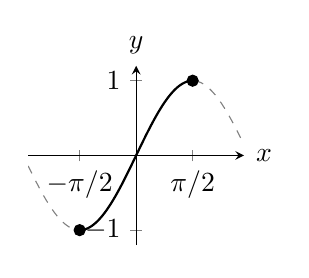
\begin{tikzpicture}
			\begin{axis}[
				scale = 0.4,
				axis x line = middle,
				axis y line = middle,
				xmin = -3,
				xmax = 3,
				ymin = -1.2,
				ymax = 1.2,
				xlabel = $x$,
				ylabel = $y$,
				xtick = {-1.571, 1.571},
				xticklabels = {$-\pi/2$, $\pi/2$},
				ytick = {-1, 1},
				yticklabels = {$-1$, $1$},
				every axis x label/.style = {
					at = {(ticklabel* cs:1.01)},
					anchor = west,
				},
				every axis y label/.style = {
					at = {(ticklabel* cs:1.01)},
					anchor = south,
				},
				]
				\addplot[
				gray,
				dashed,
				samples = 100,
				domain = -3:3,
				]{sin((x)r)};
				\addplot[
				black,
				thick,
				samples = 100,
				domain = -1.571:1.671,
				]{sin((x)r)};
				\addplot[mark=*] coordinates {(-1.571, -1)};
				\addplot[mark=*] coordinates {(1.571, 1)};
			\end{axis}
		\end{tikzpicture}
		\caption{Sine}
	\end{subfigure}
	\quad
	\begin{subfigure}{0.3\textwidth}
		\centering
		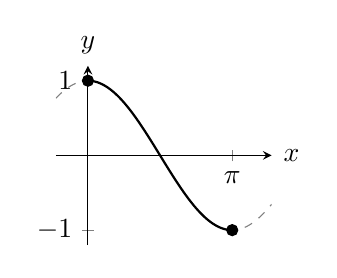
\begin{tikzpicture}
			\begin{axis}[
				scale = 0.4,
				axis x line = middle,
				axis y line = middle,
				xmin = -0.7,
				xmax = 4,
				ymin = -1.2,
				ymax = 1.2,
				xlabel = $x$,
				ylabel = $y$,
				xtick = {3.142},
				xticklabels = {$\pi$},
				ytick = {-1, 1},
				yticklabels = {$-1$, $1$},
				every axis x label/.style = {
					at = {(ticklabel* cs:1.01)},
					anchor = west,
				},
				every axis y label/.style = {
					at = {(ticklabel* cs:1.01)},
					anchor = south,
				},
				]
				\addplot[
				gray,
				dashed,
				samples = 100,
				domain = -0.7:4,
				]{cos((x)r)};
				\addplot[
				black,
				thick,
				samples = 100,
				domain = 0:3.142,
				]{cos((x)r)};
				\addplot[mark=*] coordinates {(0, 1)};
				\addplot[mark=*] coordinates {(3.142, -1)};
			\end{axis}
		\end{tikzpicture}
		\caption{Cosine}
	\end{subfigure}
	\quad
	\begin{subfigure}{0.3\textwidth}
		\centering
		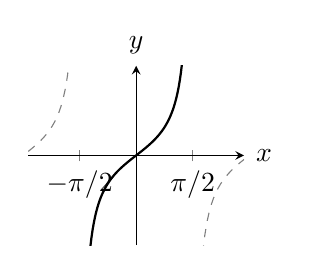
\begin{tikzpicture}
			\begin{axis}[
				scale = 0.4,
				axis x line = middle,
				axis y line = middle,
				xmin = -3,
				xmax = 3,
				ymin = -3.2,
				ymax = 3.2,
				xlabel = $x$,
				ylabel = $y$,
				xtick = {-1.571, 1.571},
				xticklabels = {$-\pi/2$, $\pi/2$},
				ytick = \empty,
				every axis x label/.style = {
					at = {(ticklabel* cs:1.01)},
					anchor = west,
				},
				every axis y label/.style = {
					at = {(ticklabel* cs:1.01)},
					anchor = south,
				},
				restrict y to domain = -4:4
				]
				\addplot[
				gray,
				dashed,
				samples = 100,
				domain = -3:3,
				]{tan((x)r)};
				\addplot[
				black,
				thick,
				samples = 100,
				domain = -1.571:1.671,
				]{tan((x)r)};
			\end{axis}
		\end{tikzpicture}
		\caption{Tangent}
	\end{subfigure}
	\caption{Restricted domains of trigonometric functions.}
	\label{lec6:inversetrig}
\end{figure}

Of course trigonometric functions are periodic and therefore not one-to-one, so in order to invert them we restrict their domains, as demonastrated in Figure \ref{lec6:inversetrig}. We therefore have
\begin{align*}
	\arcsin(\sin(x)) & = x, \qquad -\frac{\pi}{2} \leq x \leq \frac{\pi}{2}; \\
	\sin(\arcsin(x)) & = x, \qquad -1 \leq x \leq 1;                         \\
	\arccos(\cos(x)) & = x, \qquad 0 \leq x \leq \pi;                        \\
	\cos(\arccos(x)) & = x, \qquad -1 \leq x \leq 1;                         \\
	\arctan(\tan(x)) & = x, \qquad -\frac{\pi}{2} < x < \frac{\pi}{2};       \\
	\tan(\arctan(x)) & = x, \qquad -\infty < x < \infty.
\end{align*}

\noindent
We can now find the derivatives of the inverse functions, since if $y = \arcsin(x)$, we have $x = \sin(y)$, whence
\[
	\frac{d}{d x} (x) = \frac{d}{d x} \sin(y) \quad \Longleftrightarrow 1 = \cos(y) \, \frac{d y}{d x}.
\]
Since $-\pi / 2 \leq y \leq \pi / 2$, we have $\cos(y) \geq 0$, whereby the trigonometric identity $(\cos(y))^2 + (\sin(y))^2 = 1$ is equivalent with
\[
	\cos(y) = \sqrt{1 - (\sin(y))^2} = \sqrt{1 - x^2},
\]
whence
\[
	\frac{d y}{d x} = \frac{1}{\cos(y)} = \frac{1}{\sqrt{1 - x^2}}.
\]
Note that $\arcsin$ isn't differentiable at the endpoints $x = -1$ and $x = 1$ since we get division by $0$ there, and the slope approaches infinity.

Similarly for $\arccos$ we get
\[
	\frac{d}{d x} \arccos(x) = - \frac{1}{\sqrt{1 - x^2}}
\]
and for $\arctan$ we get
\[
	\frac{d}{d x} \arctan(x) = \frac{1}{1 + x^2}.
\]

\begin{exercise}
	Prove the above two claims about $\arccos$ and $\arctan$.
	Note that for the $\arctan$ function we will require the derivative of $\tan(x)$, which is quite useful and turns out to be $(\sec(x))^2 = 1 + (\tan(x))^2$.
\end{exercise}


\topic{The Natural Logarithm}

We will now \emph{define} a function $\ln(x)$, called the \keyword{natural logarithm}\index{natural logarithm} of $x$.
This definition might look quite strange, but we will show that it has the properties we expect of logarithms.

\begin{definition}[Natural logarithm]
	Take $x > 0$ and let $A(x)$ be defined as the area of the plane bounded by the curve $y = 1/t$, the $t$ axis, and the vertical lines $t = 1$ and $t = x$ (see Figure \ref{lec6:lndef}).

	The function $\ln$ is defined as
	\[
		\ln(x) = \begin{cases}
		A(x), & \text{if}~ x \geq 1 \\
		- A(x), & \text{if}~ 0 < x < 1.
		\end{cases}
	\]
\end{definition}

\begin{figure}
	\centering
	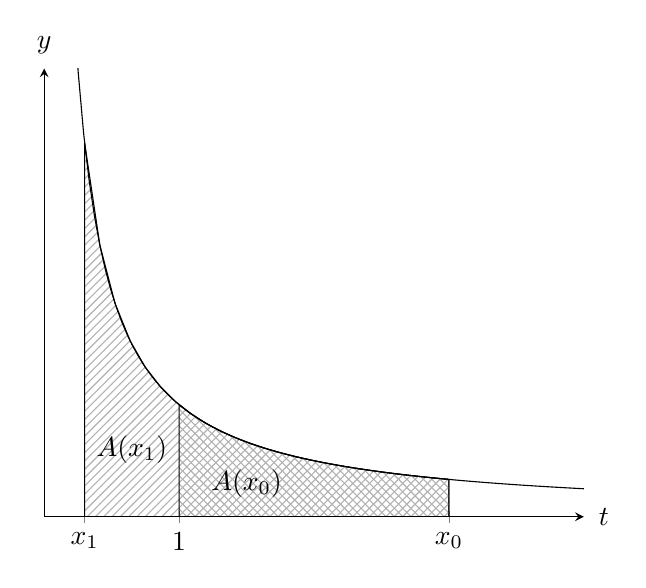
\begin{tikzpicture}
		\begin{axis}[
			scale = 1,
			axis x line = left,
			axis y line = left,
			xmin = 0,
			xmax = 4,
			ymin = 0,
			ymax = 4,
			xlabel = $t$,
			ylabel = $y$,
			xtick = {0.3, 1, 3},
			xticklabels = {$x_1$, $1$, $x_0$},
			ytick = \empty,
			every axis x label/.style = {
				at = {(ticklabel* cs:1.01)},
				anchor = west,
			},
			every axis y label/.style = {
				at = {(ticklabel* cs:1.01)},
				anchor = south,
			},
			restrict y to domain = 0:10
			]
			\addplot[
			black,
			pattern color = gray!60,
			pattern = north east lines,
			domain = 0.3:3
			]{1/x} \closedcycle;
			\addplot[
			black,
			pattern color = gray!60,
			pattern = north west lines,
			domain = 1:3
			]{1/x} \closedcycle;
			\addplot[
			black,
			samples = 100,
			domain = 0.01:4
			]{1/x};
			\addplot[mark=none] coordinates {(0.65, 0.6)} node{$\!A(x_1)\!$};
			\addplot[mark=none] coordinates {(1.5, 0.3)} node{$\!A(x_0)\!$};
		\end{axis}
	\end{tikzpicture}
	\caption{The area under $y = 1/t$.}
	\label{lec6:lndef}
\end{figure}

\noindent
From the definition it follows that $\ln(1) = 0$, $\ln(x) > 0$ if $x > 1$, and $\ln(x) < 0$ if $0 < x < 1$.
Finally since the area must increase as we move $x_0$ rightward on the figure, the function is increasing, and so injective (one-to-one).

This function has a plethora interesting properties, maybe chief amongst which is

\begin{theorem}
	If $x > 0$, then
	\[
		\frac{d}{d x} \ln(x) = \frac{1}{x}.
	\]
\end{theorem}

\begin{proof}
	If $x > 0$ and $h > 0$, then $\ln(x + h) - \ln(x)$ is the area bounded by $y = 1/t$, $y = 0$, $t = x$, and $t = x + h$, as illustrated in Figure \ref{lec6:lnareasdiff}.

	\begin{figure}[b]
		\centering
		\begin{subfigure}{0.45\textwidth}
			\centering
			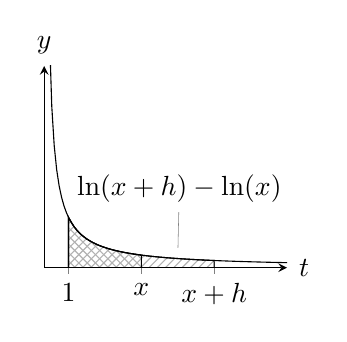
\begin{tikzpicture}
				\begin{axis}[
					scale = 0.45,
					axis x line = left,
					axis y line = left,
					xmin = 0,
					xmax = 10,
					ymin = 0,
					ymax = 4,
					xlabel = $t$,
					ylabel = $y$,
					xtick = {1, 4, 7},
					xticklabels = {$1$, $x$, $x + h$},
					ytick = \empty,
					every axis x label/.style = {
						at = {(ticklabel* cs:1.01)},
						anchor = west,
					},
					every axis y label/.style = {
						at = {(ticklabel* cs:1.01)},
						anchor = south,
					},
					restrict y to domain = 0:10
					]
					\addplot[
					black,
					pattern color = gray!60,
					pattern = north east lines,
					domain = 1:7
					]{1/x} \closedcycle;
					\addplot[
					black,
					pattern color = gray!60,
					pattern = north west lines,
					domain = 1:4
					]{1/x} \closedcycle;
					\addplot[
					black,
					samples = 100,
					domain = 0.01:10
					]{1/x};
					\addplot[mark=none] coordinates {(5.5, 0.2)} node[pin=88:{$\ln(x+h) - \ln(x)$}]{};
				\end{axis}
			\end{tikzpicture}
			\caption{The area $\ln(x + h) - \ln(x)$.}
			\label{lec6:lnareasdiff}
		\end{subfigure}
		\quad
		\begin{subfigure}{0.45\textwidth}
			\centering
			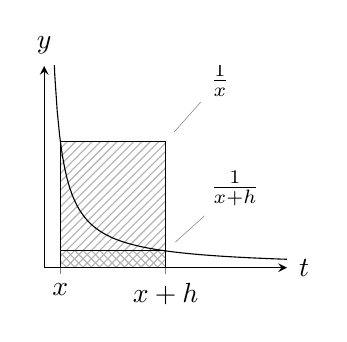
\begin{tikzpicture}
				\begin{axis}[
					scale = 0.45,
					axis x line = left,
					axis y line = left,
					xmin = 0,
					xmax = 3,
					ymin = 0,
					ymax = 8,
					xlabel = $t$,
					ylabel = $y$,
					xtick = {0.2, 1.5},
					xticklabels = {$x$, $x + h$},
					ytick = \empty,
					every axis x label/.style = {
						at = {(ticklabel* cs:1.01)},
						anchor = west,
					},
					every axis y label/.style = {
						at = {(ticklabel* cs:1.01)},
						anchor = south,
					},
					restrict y to domain = 0:10
					]
					\addplot[
					black,
					pattern color = gray!60,
					pattern = north east lines,
					domain = 0.2:1.5
					]{5} \closedcycle;
					\addplot[
					black,
					pattern color = gray!60,
					pattern = north west lines,
					domain = 0.2:1.5
					]{0.6667} \closedcycle;
					\addplot[
					black,
					samples = 100,
					domain = 0.01:3
					]{1/x};
					\addplot[mark=none] coordinates {(1.5, 0.6667)} node[pin=45:{$\frac{1}{x + h}$}]{};
					\addplot[mark=none] coordinates {(1.5, 5)} node[pin=45:{$\frac{1}{x}$}]{};
				\end{axis}
			\end{tikzpicture}
			\caption{The area $\ln(x + h) - \ln(x)$.}
			\label{lec6:lnareasbound}
		\end{subfigure}
		\caption{The area under $y = 1/t$.}
		\label{lec6:lnareas}
	\end{figure}

	Clearly this area is greater than $h \cdot \frac{1}{x + h}$ and smaller than $h \cdot \frac{1}{x}$, as illustrated in Figure \ref{lec6:lnareasbound}, meaning that
	\begin{equation}\label{lec6:eq:lnbound}
		\frac{h}{x + h} < \ln(x + h) - \ln(x) < \frac{h}{x}.
	\end{equation}

	\noindent
	If we divide this through by $h$ (which is positive by assumption) we get
	\[
		\frac{1}{x + h} < \frac{\ln(x + h) - \ln(x)}{h} < \frac{1}{x},
	\]
	which by the Squeeze theorem (for one-sided limits) gives
	\[
		\lim_{h \to 0^+} \frac{\ln(x + h) - \ln(x)}{h} = \frac{1}{x}
	\]
	since
	\[
		\lim_{h \to 0^+} \frac{1}{x + h} = \lim_{h \to 0^+} \frac{1}{x} = \frac{1}{x}.
	\]

	\noindent
	Taking $h < 0$ instead (and we also need to guarantee that $x + h > 0$, so take $h$ such that $0 < x + h < x$) we get the following from Equation \eqref{lec6:eq:lnbound}:
	\[
		\frac{1}{x} < \frac{\ln(x + h) - \ln(x)}{h} < \frac{1}{x + h},
	\]
	which by the same argument yields
	\[
		\lim_{h \to 0^-} \frac{\ln(x + h) - \ln(x)}{h} = \frac{1}{x},
	\]
	so in all
	\[
		\frac{d}{d x} \ln(x) = \lim_{h \to 0} \frac{\ln(x + h) - \ln(x)}{h} = \frac{1}{x}. \qedhere
	\]
\end{proof}

\noindent
Note, by the way, that $1 / x > 0$ for all $x > 0$, which is therefore another way to see that $\ln$ is increasing.

Other interesting properties of the $\ln$ function are those we associate with logarithms:

\begin{theorem}
	If $x$ and $y$ are positive, then
	\begin{romanlist}
		\item $\ln(x y) = \ln(x) + \ln(y)$;
		\item $\ln(x / y) = \ln(x) - \ln(y)$, with the special case $\ln(1 / x) = - \ln(x)$;
		\item $\ln(x^r) = r \ln(x)$, for now assuming $r \in \Q$.\footnote{This is because we have not yet showed that arbitrary exponentials are continuous.
		If they are, we could define $\ln(x^\alpha)$ for $\alpha \in \R$ to be $\lim\limits_{r \in \Q,\, r \to \alpha} \ln(x^r)$, but we can't take the limit inside the exponential until we know it is continuous.}
	\end{romanlist}
\end{theorem}

\begin{proof}
	\fakeitem{1} Let $y > 0$ be constant.
	Then by the chain rule
	\[
		\frac{d}{d x} (\ln(x y) - \ln(x)) = \frac{y}{x y} - \frac{1}{x} = 0
	\]
	for all $x > 0$.
	Since the derivative is $0$ for all $x > 0$,
	\begin{equation}\label{lec6:eq:lnmult}
		\ln(x y) - \ln(x) = C
	\end{equation}
	must be constant by Theorem \ref{lec5:constantfunction} last lecture.
	Take $x = 1$, then $\ln(y) - 0 = C$, so $C = \ln(y)$, whence Equation \eqref{lec6:eq:lnmult} gives
	\[
		\ln(x y) = \ln(x) + \ln(y).
	\]

	\fakeitem{2} Consider
	\[
		\frac{d}{d x} \ln \Big ( \frac{1}{x} \Big ) = \frac{1}{1 / x} \cdot - \frac{1}{x^2} = - \frac{1}{x}.
	\]
	So mimicking \fakeitemref{1}, look at $\ln(1 / x) + \ln(x)$ since
	\[
		\frac{d}{d x} \Big ( \ln \big ( \frac{1}{x} \big ) + \ln(x) \Big ) = - \frac{1}{x} + \frac{1}{x} = 0,
	\]
	so $\ln(1 / x) + \ln(x) = C$ is constant, and in particular $C = 0$ (to see this, take $x = 1$).
	Therefore
	\[
		\ln \Big ( \frac{1}{x} \Big ) = - \ln(x).
	\]
	To finish the proof, take this together with \fakeitemref{1}.

	\fakeitem{3} In the same way, study
	\[
		\frac{d}{d x} \ln(x^r) = \frac{1}{x^r} \cdot r x^{r - 1} = r \cdot x^{r - 1 - r} = \frac{r}{x},
	\]
	at least for $r \in \Q$ so far, whereby
	\[
		\frac{d}{d x} \big ( \ln(x^r) - r \ln(x) \big ) = 0,
	\]
	so $\ln(x^r) - r \ln(x) = C$ for every $x$.
	Plugging in $x = 1$ gives $C = 0$, whence
	\[
		\ln(x^r) = r \ln(x). \qedhere
	\]
\end{proof}

\topic{The Exponential Function}

Since $\ln \colon \R_{> 0} \to \R$ is injective and clearly\footnote{Hopefully. Think about it!} surjective, it is bijective and therefore has an inverse function.
We call this inverse function the \keyword{exponential function}\index{exponential function}, $\exp \colon \R \to \R_{> 0}$,
\[
	y = \exp(x) \qquad \Longleftrightarrow \qquad x = \ln(y),
\]
for $y > 0$.
We already know a bit about this function.
Since $\ln(1) = 0$, we also have $\exp(0) = 1$.
Since it's an inverse, we have
\[
	\ln(\exp(x)) = x
\]
for all $x \in \R$ and
\[
	\exp(\ln(x)) = x
\]
for all $x > 0$.

Due to the last theorem we can also quickly deduce a few more properties of this function:

\begin{theorem}
	If $x$ and $y$ are any real numbers, then
	\begin{romanlist}
		\item $(\exp(x))^r = \exp(r x)$;
		\item $\exp(x + y) = \exp(x) \exp(y)$;
		\item $\exp(x - y) = \exp(x) / \exp(y)$, with the special case $\exp(-x) = 1 / \exp(x)$.
	\end{romanlist}
\end{theorem}

\begin{proof}
	We use that it is the inverse of $\ln$ alongside the previous theorem.

	\fakeitem{1} If $y = (\exp(x))^r$, then $\ln(y) = \ln(\exp(x)^r) = r \ln(\exp(x)) = rx$, whereby if we take exponents of both sides gives us $y = \exp(r x)$.

	\fakeitem{2} Take $z = \exp(x + y)$, which is equivalent with
	\[
		\ln(z) = x + y = \ln(\exp(x)) + \ln(\exp(y)) = \ln(\exp(x) \exp(y)).
	\]
	Now take exponents of both sides to get $z = \exp(x) \exp(y)$.

	\fakeitem{3} Same idea: $y = \exp(-x)$ is equivalent with
	\[
		\ln(y) = -x = - \ln(\exp(x)) = \ln \Big ( \frac{1}{\exp(x)} \Big ).
	\]
	Again the more general result follows from this together with \fakeitemref{2}.
\end{proof}



\lecture[February 6, 2017]{The Number $e$ and L'H\^{o}pital's Rules}

\topic{The Number $e$}

We now \emph{define} the number $e = \exp(1)$\index{e@$e$}, in other words $\ln(e) = 1$, making $e$ the \emph{unique} number that makes the area under $1 / t$ precisely $1$.

Now comes a \emph{crucial} point: $\exp(x)$ is defined for \emph{all} $x \in \R$ (since it is the inverse of $\ln$), so we can extend
\[
	\exp(r) = \Big ( \exp(1 \cdot r) = \exp(1)^r \Big ) = e^r
\]
to be defined not only for $r \in \Q$, but for all $r$!
Note that this is not an equality we prove, but a definition we take.
We therefore \emph{define}
\[
	e^x = \exp(x)
\]
for all $x \in \R$.

This is a very special function, for it is the only (nontrivial) function which is its own derivative everywhere.

\begin{theorem}
	$\displaystyle \frac{d}{d x} e^x = e^x$.
\end{theorem}

\begin{proof}
	By defintion $y = e^x$ is equivalent with $x = \ln(y)$.
	If we differentiate this implicitly we get
	\[
		1 = \frac{1}{y} \cdot \frac{d y}{d x},
	\]
	which yields
	\[
		y = \frac{d y}{d x} = e^x. \qedhere
	\]
\end{proof}

\noindent
The fact that $e^x$ is now defined for all $x$ helps us to define arbitrary exponentials $a^x$, for $a > 0$.
For rational $r$ we have
\[
	\ln(a^r) = r \ln(a),
\]
which is equivalent with
\[
	a^r = e^{r \ln(a)}.
\]
Notice how the right-hand side is defined for all $r$, since $e^x$ is, so we take this as the definition of $a^r$ for all $r \in \R$, with no contradiction arising if $r \in \Q$.

\begin{definition}
	Let $a > 0$ and $x \in \R$.
	Then
	\[
		a^x = e^{x \ln(a)}
	\]
	by definition.
\end{definition}

\noindent
Using the chain rule we can now compute
\[
	\frac{d}{d x} \, a^x = \frac{d}{d x} \, e^{x \ln(a)} = e^{x \ln(a)} \cdot \ln(a) = a^x \ln(a).
\]

\noindent
Moreover we are finally able to prove the general power rule for derivatives:

\begin{proposition}
	Provided $x > 0$ and $\alpha \in \R$, we have
	\[
		\frac{d}{d x} \, x^\alpha = \alpha x^{\alpha - 1}.
	\]
\end{proposition}

\begin{proof}
	Straight forward computation by writing $x^\alpha = e^{\alpha \ln(x)}$:
	\[
		\frac{d}{d x} \, x^\alpha = \frac{d}{d x} \, e^{\alpha \ln(x)} = e^{\alpha \ln(x)} \cdot \frac{\alpha}{x} = x^\alpha \cdot \alpha \cdot x^{-1} = \alpha x^{\alpha - 1}.\qedhere
	\]
\end{proof}

\noindent
We can go further.
Our exponential $e^x$ is continuous everywhere (since it has a derivative everywhere), whereby we can finally prove for all $\alpha \in \R$ that
\[
	\lim_{x \to c} \big ( f(x) \big )^\alpha = \Big ( \lim_{x \to c} f(x) \Big )^\alpha,
\]
provided $\lim\limits_{x \to c} f(x) > 0$.
Namely since now by definition $(f(x))^\alpha = e^{\alpha \ln(f(x))}$, so
\[
	\lim_{x \to c} \big ( f(x) \big )^\alpha = e^{\lim\limits_{x \to c} (\alpha \ln(f(x)))} = e^{\alpha \ln \big ( \lim\limits_{x \to c} f(x) \big )} = \Big ( \lim_{x \to c} f(x) \Big )^\alpha.
\]

\begin{example}
	Compute $f'(x)$ when $f(x) = x^x$.

	Neither $(a^x)' = a^x \ln(a)$ nor $(x^a)' = a x^{a - 1}$ apply (why?).

	On the other hand,
	\[
		\frac{d}{d x} \, x^x = \frac{d}{d x} \, e^{x \ln(x)} = e^{x \ln(x)} \cdot \Big ( x \cdot \frac{1}{x} + \ln(x) \Big ) = x^x (1 + \ln(x)). \qedhere
	\]
\end{example}

\topic{How Fast is Exponential and Logarithmic Growth?}

Both exponential and logarithmic growth approach infinity, but we ask ourselves how quickly.
In fact, $e^x$ grows faster than any positive power, and $\ln(x)$ increases more slowly than any positive power. To show this and to compute some useful limits, we first show that $\ln(x) \leq x - 1$ for all $x > 0$:

Let $g(x) = \ln(x) - (x - 1)$ for $x > 0$.
We have $g(1) = 0$, and $g'(x) = 1/x - 1$, which is positive for $0 < x < 1$ and negative for $x > 1$.

Therefore $g(x)$ is increasing on ${]{0, 1}[}$ and decreasing on ${]{1, \infty}[}$, whence $g(x) \leq g(1) = 0$ for all $x > 0$, meaning that $\ln(x) - (x - 1) \leq 0$, which by adding $x - 1$ to both sides yields $\ln(x) \leq x - 1$.

This method of studying the derivative of the difference of two functions is a very effective method to show that one function is greater than or less than another function.

\begin{theorem}
	If $a > 0$, then
	\begin{romanlist}
		\item $\displaystyle \lim_{x \to \infty} \frac{\ln(x)}{x^a} = 0$,
		\item $\displaystyle \lim_{x \to 0^+} x^a \ln(x) = 0$,
		\item $\displaystyle \lim_{x \to \infty} \frac{x^a}{e^x} = 0$,
		\item $\displaystyle \lim_{x \to -\infty} \abs{x}^a e^x = 0$.
	\end{romanlist}
\end{theorem}

\begin{proof}
	\fakeitem{1} Let $x > 1$, $a > 0$, and $s = a / 2$.
	Since $\ln(x^s) = s \ln(x)$, our above result $\ln(x) \leq x - 1$ gives us $\ln(x^s) = s \ln(x) \leq x^s - 1 < x^s$, which dividing by $s$ produces
	\[
		0 < \ln(x) < \frac{x^s}{s}.
	\]
	By dividing again by $x^a = x^{2 s}$ we arrive at
	\[
		0 < \frac{\ln(x)}{x^a} < \frac{x^s}{s x^{2 s}} = \frac{1}{s x^s}.
	\]
	Now
	\[
		\lim_{x \to \infty} \frac{1}{s} \, \frac{1}{x^s} = 0
	\]
	since $s > 0$, so by the Squeeze theorem
	\[
		\lim_{x \to \infty} \frac{\ln(x)}{x^a} = 0
	\]
	as well.

	\fakeitem{2} We use \fakeitemref{1} and substitute $x = 1/t$.
	Then as $x \to 0^+$ we have $t \to \infty$, whereby
	\[
		\lim_{x \to 0^+} x^a \ln(x) = \lim_{t \to \infty} \frac{\ln(1 / t)}{t^a} = - \lim_{t \to \infty} \frac{\ln(t)}{t^a} = -0 = 0.
	\]

	\noindent
	\fakeitem{3} Again in \fakeitemref{1}, substitute $x = \ln(t)$, so that $t \to \infty$ corresponds to $x \to \infty$,
	\[
		\lim_{x \to \infty} \frac{x^a}{e^x} = \lim_{t \to \infty} \frac{(\ln(t))^a}{t} = \lim_{t \to \infty} \Big ( \frac{\ln(t)}{t^{1/a}} \Big ) ^a = 0^a = 0.
	\]

	\noindent
	\fakeitem{4} Finally in \fakeitemref{3} we substitute $x = -t$:
	\[
		\lim_{x \to -\infty} \abs{x}^a e^x = \lim_{t \to \infty} \abs{- t}^a e^{-t} = \lim_{t \to \infty} \frac{t^a}{e^t} = 0. \qedhere
	\]
\end{proof}

\noindent
Another interesting limit, and one which is sometimes taken to be the definition of $e$, is
\begin{theorem}
	For every real $x$,
	\[
		e^x = \lim_{n \to \infty} \Big ( 1 + \frac{x}{n} \Big )^n.
	\]
\end{theorem}

\begin{proof}
	For $x = 0$ it is trivially true.

	For $x \neq 0$, take $y = x / n$, with $x$ being fixed.
	Clearly $y$ tends to $0$ as $n$ tends to infinity, whereby
	\begin{align*}
		\lim_{n \to \infty} \ln \Big ( \Big ( 1 + \frac{x}{n} \Big )^n \Big ) & = \lim_{n \to \infty} n \ln\Big ( 1 + \frac{x}{n} \Big ) = \lim_{n \to \infty} \frac{\frac{x}{n} n \ln \big ( 1 + \frac{x}{n} \big )}{x / n} \\
		                                                                      & = x \lim_{y \to 0} \frac{\ln(1 + y)}{y} = x \lim_{y \to 0} \frac{\ln(1 + y) - \ln(1)}{y},
	\end{align*}
	which is of course $x f'(1)$ where $f(x) = \ln(x)$, so the limit is $x \cdot 1/1 = x$.
	Since $\ln(x)$ is continuous, we can take limits in and out of it, so the above becomes
	\[
		\lim_{n \to \infty} \ln \Big ( \Big ( 1 + \frac{x}{n} \Big )^n \Big ) = \ln \Big ( \lim_{n \to \infty} \Big ( 1 + \frac{x}{n} \Big )^n \Big ) = x.
	\]
	Taking exponentials we arrive at
	\[
		e^x = \lim_{n \to \infty} \Big ( 1 + \frac{x}{n} \Big )^n. \qedhere
	\]
\end{proof}

\topic{Intermediate Forms and L'H\^{o}pital's Rules}

Recall how some time ago we computed
\[
	\lim_{x \to 0} \frac{\sin(x)}{x} = 1,
\]
despite $\sin(x) \to 0$ and $x \to 0$ as $x \to 0$.
We call $\sin(x) / x$ an \keyword{intermediate form}\index{intermediate form} of the type ``$0 / 0$'' or $[0 / 0]$, depending on the textbook.

The reason we call this an intermediate form is that a limit approaching $0 / 0$ can be equal to anything, or indeed not exist at all.

\begin{examples}
	Consider the following limits:
	\[
		\lim_{x \to 0} \frac{k x}{x} = k, \quad \lim_{x \to 0} \frac{x}{x^3} = \infty, \quad \text{and} \quad \lim_{x \to 0} \frac{x^3}{x^2} = 0. \qedhere
	\]
\end{examples}

\noindent
There are other types of intermediate forms:
\[
	``\infty / \infty ", \quad ``0 \cdot \infty", \quad ``\infty - \infty", \quad ``0^0", \quad ``\infty^0", \quad \text{and} \quad ``1^\infty".
\]
We saw a few of these, in particular the first two, in the logarithm and exponential limits.

Encountering ``$0 / 0$'' is perhaps the most common, and they can often be resolved by simplifying or using the Squeeze theorem.

Another method for computing limits of the form ``$0 / 0$'' or ``$\infty / \infty$'' are the two l'H\^{o}pital's rules. Most other forms can be made into these two forms by some algebraic manipulation of change of variable.

\begin{theorem}[L'H\^{o}pital's first rule]
	Suppose $f$ and $g$ are differentiable on ${]{a, b}[}$, and
	\[
		\lim_{x \to a^+} f(x) = \lim_{x \to a^+} g(x) = 0.
	\]
	If $g'(x) \neq 0$ for all $x \in {]{a, b}[}$, and the limit
	\[
		\lim_{x \to a^+} \frac{f'(x)}{g'(x)} = L
	\]
	exists, then $g(x) \neq 0$ for all $x \in {]{a, b}[}$ and
	\[
		\lim_{x \to a^+} \frac{f(x)}{g(x)} = L.
	\]
\end{theorem}

\begin{remark}
	The same holds for left limits, two-sided limits, and limits at $\pm \infty$, assuming $f$ and $g$ are differentiable on the relevant punctured neighbourhoods.
\end{remark}

\begin{proof}
	This proof is based on defining continuous extensions of $f$ and $g$, namely $F(x) = f(x)$ and $G(x) = g(x)$ for $a < x < b$ and $F(a) = G(a) = 0$.
	Then $F$ and $G$ are continuous on $[a, x]$ for all $a < x < b$.
	By the Mean-value theorem,
	\[
		g(x) = G(x) - G(a) = g'(c) (x - a)
	\]
	for some $c \in {]{a, x}[}$, so since $g'(c) \neq 0$ by assumption, we must have $g(x) \neq 0$ for all $a < x < b$, since the right-hand side is never $0$.

	By the Generalised mean-value theorem, for each $x \in {]{a, b}[}$, there exists a $c \in {]{a, x}[}$ (depending on $x$) such that
	\[
		\frac{f(x)}{g(x)} = \frac{F(x)}{G(x)} = \frac{F(x) - F(a)}{G(x) - G(a)} = \frac{f'(c)}{g'(c)}.
	\]
	Now since $a < c < x$, $c$ will approach $a$ from above as $x$ does.
	Therefore
	\[
		\lim_{x \to a^+} \frac{f(x)}{g(x)} = \lim_{c \to a^+} \frac{f'(c)}{g'(c)} = L. \qedhere
	\]
\end{proof}

\noindent
The proof for the left-hand limits is almost identical, and the two-sided result is just the combination of the two.

For limits at $\pm\infty$, we take $y = 1/x$ and study the functions $F(y) = f(1/y)$ and $G(y) = g(1/y)$.
Then
\[
	F'(y) = - \frac{f'(1/y)}{y^2} \qquad \text{and} \qquad G'(y) = - \frac{g'(1 / y)}{y^2},
\]
so
\[
	\frac{F'(y)}{G'(y)} = \frac{f'(1/y)}{g'(1/y)},
\]
whereby
\[
	\lim_{x \to \pm\infty} \frac{f(x)}{g(x)} = \lim_{y \to 0^\pm} \frac{F(y)}{G(y)} = \lim_{y \to 0^\pm} \frac{F'(y)}{G'(y)} = \lim_{x \to \pm\infty} \frac{f'(x)}{g'(x)}.
\]

\noindent
The second rule of H\^{o}pital concerns the ``$\infty / \infty$'' case:

\begin{theorem}[L'H\^{o}pital's second rule]
	L'H\^{o}pital's rule also holds if we have $\lim \abs{f(x)} = \lim \abs{g(x)} = \infty$.
\end{theorem}

\begin{proof}
	We'll consider limits as $x \to a^-$.
	The other cases follow in the same was as described above.

	Let $\varepsilon > 0$.
	We want to show that
	\[
		\abs[\Big]{\frac{f(x)}{g(x)} - L} < \varepsilon
	\]
	if $a - x < \delta$ for some $\delta > 0$.
	Since
	\[
		\frac{f'(x)}{g'(x)} \to L
	\]
	and $\abs{g(x)} \to \infty$ as $x \to a^-$, we can pick an $x_0 < a$ in such a way that $\abs{f'(x) / g'(x) - L} < \varepsilon/2$ and $g(x) \neq 0$ for all $x \in {]{x_0, a}[}$.
	The Generalised mean-value theorem gives
	\[
		\frac{f(x) - f(x_0)}{g(x) - g(x_0)} = \frac{f'(c)}{g'(c)}
	\]
	for some $x_0 < c < x$, meaning that
	\begin{equation}\label{lec7:eq:lhopitals}
		\abs[\Big]{\frac{f(x) - f(x_0)}{g(x) - g(x_0)} - L} < \frac{\varepsilon}{2}
	\end{equation}
	for $x_0 < x < a$ since $x_0 < c < a$.

	By some algebraic manipulation we have
	\[
		\frac{f(x) - f(x_0)}{g(x) - g(x_0)} = \frac{\frac{f(x)}{g(x)} - \frac{f(x_0)}{g(x)}}{1 - \frac{g(x_0)}{g(x)}},
	\]
	which if solved for $f(x)/g(x)$ becomes
	\[
		\frac{f(x)}{g(x)} = \frac{f(x) - f(x_0)}{g(x) - g(x_0)} - \frac{f(x) - f(x_0)}{g(x) - g(x_0)} \cdot \frac{g(x_0)}{g(x)} + \frac{f(x_0)}{g(x)}.
	\]

	\noindent
	As $x$ tends to $a$ from below, $\abs{g(x)} \to \infty$ by assumption, so $f(x_0) / g(x)$ and $g(x_0) / g(x)$ tend to $0$, so the last two terms tend to $0$ since the difference quotient is bounded by Equation \eqref{lec7:eq:lhopitals}.

	Thus for $x$ sufficiently close to $a$ from below,
	\[
		\abs[\Big]{\frac{f(x)}{g(x)} - \frac{f(x) - f(x_0)}{g(x) - g(x_0)}} < \frac{\varepsilon}{2}.
	\]

	\noindent
	Adding this and Equation \eqref{lec7:eq:lhopitals} together yields
	\[
		\abs[\Big]{\frac{f(x) - f(x_0)}{g(x) - g(x_0)} - L} + \abs[\Big]{\frac{f(x)}{g(x)} - \frac{f(x) - f(x_0)}{g(x) - g(x_0)}}  < \varepsilon,
	\]
	so by using the Triangle inequality backwards we have
	\[
		\abs[\Big]{\frac{f(x)}{g(x)} - L} < \varepsilon. \qedhere
	\]
\end{proof}



\lecture[February 9, 2017]{Sketching Functions}

%!TEX root = ../lectures.tex

\topic{Extreme Values}

As we saw when discussing the Mean-value theorem, the sign of the derivative tells us whether the function is increasing or decreasing.
We will now explore how to use this information to find maximum and minimum values, collectively known as \keyword{extreme values}\index{extreme value}.

Recall how a function has an \keyword{absolute}\index{absolute maximum|see {global maximum}} or \keyword{global maximum value}\index{global maximum} $f(x_0)$ at $x = x_0$ if $f(x) \leq f(x_0)$ for all $x$ in the domain of $f$.

(Similarly it has an \keyword{absolute}\index{absolute minimum|see {global min}} or \keyword{global minimum value}\index{global minimum} if $f(x) \geq f(x_0)$.)

Note that a function can have at most one global maximum value, and at most one global minimum value, but they can attain these values for more than one $x$-value.

\begin{example}
	The function $f(x) = \sin(x)$ attains its global maximum value $1$ at $x = \pi/2 + 2 \pi n$ and its global minimum value $-1$ at $x = -\pi/2 + 2 \pi n$, for $n \in \Z$.
\end{example}

\noindent
Functions don't always have global extreme values.

\begin{example}
	The function plotted in Figure \ref{lec7:globalextreme} has no global maximum value, since it goes off to infinity close to the dashed line, however it does have a \keyword{local maximum value} in the right part.
\end{example}

\begin{figure}[b!]
	\centering
	\begin{tikzpicture}
		\begin{axis}[
			scale = 1,
			axis x line = left,
			axis y line = left,
			xmin = 0,
			xmax = 4,
			ymin = 0,
			ymax = 10,
			xlabel = $x$,
			ylabel = $y$,
			xtick = \empty,
			ytick = \empty,
			every axis x label/.style = {
				at = {(ticklabel* cs:1.01)},
				anchor = west,
			},
			every axis y label/.style = {
				at = {(ticklabel* cs:1.01)},
				anchor = south,
			},
			restrict y to domain = 0:10
			]
			\addplot[
			black,
			samples = 100,
			domain = 0.5:1.999
			]{1/((x-2.25)^2)};
			\addplot[
			black,
			samples = 100,
			domain = 2:3.6
			]{sin((3*x)r)+2};
			\addplot[
			gray,
			dashed,
			] coordinates {(2, 0) (2, 9.5)};
			\addplot[mark=*] coordinates {(0.5, 0.3265)};
			\addplot[mark=o] coordinates {(2, 1.7206)};
			\addplot[mark=*] coordinates {(3.6, 1.0191)};
		\end{axis}
	\end{tikzpicture}
	\caption{A function with no global maximum.}
	\label{lec7:globalextreme}
\end{figure}

\begin{definition}[Local extreme values]
	A function $f$ has a \keyword{local maximum value}\index{local maximum value} $f(x_0)$ at $x_0$ in its domain if there exists a number $h > 0$ such that $f(x) \leq f(x_0)$ whenever $x$ is in the domain of $f$ and $\abs{x - x_0} < h$.

	Similarly for \keyword{local minimum value}, with $f(x) \geq f(x_0)$.
\end{definition}

\noindent
A function $f$ can have local extreme values only at points of three special types:
\begin{romanlist}
	\item \keyword{critical points}\index{critical point} of $f$, i.e. points of the domain where $f'(x) = 0$;
	\item \keyword{singular points}\index{singular points} of $f$, i.e. points of the domain where $f'(x)$ is undefined; and
	\item \keyword{endpoints} of the domain of $f$, i.e. points of the domain that do not belong to any open interval contained in the domain of $f$.
\end{romanlist}

\noindent
The first item about critical points follows from Lemma \ref{lec4:criticalpoint} related to the Mean-value theorem, and the others are fairly obvious.

A point being a local extreme value implies \fakeitemref{1}, \fakeitemref{2}, or \fakeitemref{3}, but the other way around need not be true; critical points, singular points and endpoints need not be extreme points.

\begin{counterexample}
	Consider the function $f(x) = x^3$.
	We have $f'(x) = 3 x^2$, whence $f'(0) = 0$, so by definition $x = 0$ is a critical point, yet $f(0) = 0$ is no local extreme value.
\end{counterexample}

\noindent
We can decide whether the three types of points are local minimum or maximum values by studying the derivative close to the points.

\begin{theorem}[First derivative test]
	Let $f \colon X \to Y$ be a function differentiable on the relevant intervals below.
	The theorem has two parts:

	\subsubsection*{Testing critical and singular points}

	Suppose $f$ is continuous at $x_0$ and that $x_0$ isn't an endpoint of $X$.
	\begin{romanlist}
		\item If there exists an open interval $\interval[open]{a}{b} \ni x_0$ such that $f'(x) > 0$ on $\interval[open]{a}{x_0}$ and $f'(x) < 0$ on $\interval[open]{x_0}{b}$, then $f$ has a local maximum value at $x_0$.
		\item Similarly $f$ has a local minimum value at $x_0$ if $f'(x) < 0$ on $\interval[open]{a}{x_0}$ and $f'(x) > 0$ on $\interval[open]{x_0}{b}$.
	\end{romanlist}

	\subsubsection*{Testing endpoints of $X$}

	Suppose $a$ is a left endpoint of $X$ and that $f$ is right continuous at $a$.
	\begin{romanlist}
		\setcounter{enumi}{2}
		\item If $f'(x) > 0$ on some interval $\interval[open]{a}{b}$, then $f$ has a local minimum at $a$.
		\item If $f'(x) < 0$ on some $\interval[open]{a}{b}$, then $f$ has a local maximum at $a$.
	\end{romanlist}
	Suppose $b$ is a right endpoint of $X$ and that $f$ is left continuous at $b$.
	\begin{romanlist}
		\setcounter{enumi}{4}
		\item If $f'(x) > 0$ on some $\interval[open]{a}{b}$, then $f$ has a local maximum at $b$.
		\item If $f'(x) < 0$ on some $\interval[open]{a}{b}$, then $f$ has a local minimum at $b$.
	\end{romanlist}
\end{theorem}

\begin{exercise}
	To prove this, recall Definition \ref{lec4:monotonicity}.
\end{exercise}

\noindent
Note that if $f'(x)$ has the same sign on both sides of a critical or singular point, then $f$ has neither maximum nor minimum at that point (like the $x^3$ example).

\begin{example}
	Consider
	\[
		f(x) = \frac{1}{3} x^3 - x
	\]
	defined on $[{-3}, 3]$.
	Potential extreme values are at the endpoints $x = -3$ and $x = 3$, and critical points (it has no singular points).

	We have
	\[
		f'(x) = \frac{1}{3} \cdot 3 \cdot x^2 - 1 = x^2 - 1 = (x - 1)(x + 1),
	\]
	so its critical points are $x = 1$ and $x = -1$.

	We analyse the sign of the derivative around these points:

	\bigskip

	\begin{table}[ht!]
		\centering
		\begin{tabular}{r|*{7}{c}}
			$x$     & $-3$ & $-3 < x < -1$ & $-1$ & $-1 < x < 1$ & $1$ & $1 < x < 3$ & $3$ \\ \hline
			$f'(x)$ &      & $+$           & $0$  & $-$          & $0$ & $+$         &     \\
			$f(x)$  & min  & $\nearrow$    & max  & $\searrow$   & min & $\nearrow$  & max
		\end{tabular}
	\end{table}

	\bigskip

	\noindent
	We (naturally) see the same behaviour by sketching the function:

	\bigskip

	\begin{figure}[ht!]
		\centering
		\begin{tikzpicture}
			\begin{axis}[
				scale = 1,
				axis x line = middle,
				axis y line = middle,
				xmin = -4,
				xmax = 4,
				ymin = -7,
				ymax = 7,
				xlabel = $x$,
				ylabel = $y$,
				xtick = {-3, -1, 1, 3},
				ytick = {-3, 3},
				every axis x label/.style = {
					at = {(ticklabel* cs:1.01)},
					anchor = west,
				},
				every axis y label/.style = {
					at = {(ticklabel* cs:1.01)},
					anchor = south,
				}
				]
				\addplot[
				black,
				samples = 100,
				domain = -3:3
				]{x^3/3-x};
				\addplot[mark=*] coordinates {(-3, -6)};
				\addplot[mark=*] coordinates {(3, 6)};
			\end{axis}
		\end{tikzpicture}
	\end{figure}
\end{example}

\topic{Concavity}

We can also use the second derivative to find out useful things about a function.

In particular, it tells us if the slope (i.e. derivative) is an increasing or decreasing function.
We have fancy names for these behaviours.

\begin{definition}[Concavity]
	We say that $f$ is \keyword{concave up}\index{concavity} on an open interval $I$ if it is differentiable there and the derivative $f'$ is an increasing function on $I$.
	We say that $f$ is \keyword{concave down} on $I$ if $f'$ exists and is decreasing on $I$.
\end{definition}

\begin{example}
	The function $f(x) = x^2$ is concave up on the entirety of $\R$.
\end{example}

\begin{example}
	The third degree polynomial from two examples ago is concave down on $x > 0$ and concave up on $x < 0$.
\end{example}

\noindent
This exemplifies how functions sometimes change concavity on either side of a point:

\begin{definition}[Inflection point]
	We say that $f$ has an \keyword{inflection point}\index{inflection point} at $x_0$ if $f$ has a (possibly vertical) tangent line there and the concavity is opposite on opposing sides of $x_0$.
\end{definition}

\noindent
We've already seen one example, namely $x = 0$ for $f(x) = x^3 / 3 - x$.

We demonstrate two more interesting examples that exemplify the requirement about the tangent line.

\begin{figure}
	\centering
	\begin{subfigure}{0.45\textwidth}
		\centering
		\begin{tikzpicture}
			\begin{axis}[
				scale = 0.5,
				axis x line = left,
				axis y line = left,
				xmin = 0,
				xmax = 6,
				ymin = 0,
				ymax = 10,
				xlabel = $x$,
				ylabel = $y$,
				xtick = {3},
				xticklabels = {$a$},
				ytick = \empty,
				yticklabels = {$f(a)$, $f(b)$},
				every axis x label/.style = {
					at = {(ticklabel* cs:1.01)},
					anchor = west,
				},
				every axis y label/.style = {
					at = {(ticklabel* cs:1.01)},
					anchor = south,
				},
				]
				\addplot[
				black,
				samples = 100,
				domain = 0.5:3,
				]{-(x-3)^2+7.5};
				\addplot[
				black,
				samples = 100,
				domain = 3:5.5,
				]{0.4*(x-5)^2+5.9};
				\addplot[
				gray,
				dashed
				] coordinates {(3, 0) (3, 7.5)};
			\end{axis}
		\end{tikzpicture}
		\caption{No tangent line at $x = a$}
		\label{lec7:inflectioncounter}
	\end{subfigure}
	\quad
	\begin{subfigure}{0.45\textwidth}
		\centering
		\begin{tikzpicture}
			\begin{axis}[
				scale = 0.5,
				axis x line = middle,
				axis y line = middle,
				xmin = -5,
				xmax = 5,
				ymin = -2,
				ymax = 2,
				xlabel = $x$,
				ylabel = $y$,
				xtick = \empty,
				xticklabels = {$a$, $b$},
				ytick = \empty,
				yticklabels = {$f(a)$, $f(b)$},
				every axis x label/.style = {
					at = {(ticklabel* cs:1.01)},
					anchor = west,
				},
				every axis y label/.style = {
					at = {(ticklabel* cs:1.01)},
					anchor = south,
				},
				]
				\addplot[
				black,
				samples = 100,
				domain = 0:4,
				]{x^(1/3)};
				\addplot[
				black,
				samples = 100,
				domain = -4:0,
				]{x/abs(x)*abs(x)^(1/3)};
			\end{axis}
		\end{tikzpicture}
		\caption{$f(x) = x^{1/3}$ with vertical tangent line at $x = 0$}
		\label{lec7:inflectionvertical}
	\end{subfigure}
	\caption{Counterexamples of the Mean-value theorem where essential conditions are violated.}
\end{figure}

\begin{examples}
	In Figure \ref{lec7:inflectioncounter} we see a function which changes concavity around $x = a$, however it is by definition \emph{not} an inflection point since there is no tangent line at this point.

	Moreover in Figure \ref{lec7:inflectionvertical} we demonstrate an inflection point at a point where the function at hand, $f(x) = x^{1/3}$, is not differentiable, but it has a tangent line.
	In this sense the condition on the existence of a tangent line is stronger than the existence of the derivative.
\end{examples}

\noindent
Since concavity depends on the derivative being increasing or decreasing, we can test it using the derivative of the derivative.

\begin{theorem}
	Let $f$ be a twice differentiable function on some interval $I$.
	\begin{romanlist}
		\item If $f''(x) > 0$ on the interval, then $f$ is concave up on $I$.
		\item If $f''(x) < 0$ on the interval, then $f$ is concave down on $I$.
		\item If $f$ has an inflection point at $x_0$ and $f''(x_0)$ exists, then $f''(x_0) = 0$.
	\end{romanlist}
\end{theorem}

\begin{proof}
	As suggested above, \fakeitemref{1} and \fakeitemref{2} are clear by Theorem \ref{lec4:monotonicityproof}, wherein the sign of the derivative implies that a function is increasing or decreasing.

	For \fakeitemref{3}, if $f$ has an inflection point at $x_0$ and $f''(x_0)$ exists, then $f$ must be differentiable on an open interval containing $x_0$.
	Since $f'$ is increasing on one side of $x_0$ and decreasing on the other, it must have a local extreme value at $x_0$, and therefore $f''(x_0) = 0$.
\end{proof}

\noindent
Combining this with what we know about critical points we get a very useful result.

\begin{theorem}[Second derivative test]
	Let $f$ be a twice differentiable function.

	\begin{romanlist}
		\item If $f'(x_0) = 0$ and $f''(x_0) < 0$, then $f$ has a local maximum value at $x_0$.
		\item If $f'(x_0) = 0$ and $f''(x_0) > 0$, then $f$ has a local minimum value at $x_0$.
	\end{romanlist}
\end{theorem}

\begin{proof}
	Suppose $f'(x_0) = 0$ and $f''(x_0) < 0$.
	Since
	\[
		\lim_{h \to 0} \frac{f'(x_0 + h)}{h} = \lim_{h \to 0} \frac{f'(x_0 + h) - f'(x_0)}{h} = f''(x_0) < 0,
	\]
	it follows that $f'(x_0 + h) > 0$ for all sufficiently small negative $h$.
	Thus by the first derivative test, $f$ must have a local maximum value at $x_0$.

	The case of the local minimum is similar.
\end{proof}

\begin{remark}
	If $f'(x_0) = f''(x_0) = 0$, no conclusion can be drawn from this information alone.
\end{remark}

\begin{example}
	Consider $f(x) = x^4$.
	Here $f'(0) = f''(0) = 0$, and $f(0) = 0$ is a local minimum value, whereas for $g(x) = x^3$ we also have $g'(0) = g''(0) = 0$, yet $x = 0$ is an inflection point.
\end{example}

\topic{Sketching Functions}

Combining all of this, and maybe some other things, we can quite accurately sketch graphs of functions.

\begin{example}
	Sketch
	\[
		f(x) = \frac{x^2 - 1}{x^2 - 4} = \frac{(x - 1)(x + 1)}{(x - 2)(x + 2)}.
	\]

	\noindent
	We take stock of what we know.

	The domain is all $x \neq \pm 2$.
	There are vertical asymptotes at $x = \pm 2$.
	Because
	\[
		\lim_{x \to \pm \infty} \frac{x^2 - 1}{x^2 - 4} = \lim_{x \to \pm \infty} \frac{x^2}{x^2} \cdot \frac{1 - 1/x^2}{1 - 4/x^2} = 1,
	\]
	$y = 1$ is a horizontal asymptote.

	We also observe that $f$ is even, since $f(-x) = f(x)$.

	It crosses the $x$-axis at $x = \pm 1$, and it intersects the $y$-axis at $f(0) = 1/4$.

	Finally we compute the first and second derivatives:
	\[
		f'(x) = \frac{2x \cdot (x^2 - 4) - 2x \cdot (x^2 - 1)}{(x^2 - 4)^2} = \frac{- 6x}{(x^2 - 4)^2},
	\]
	and
	\[
		f''(x) = \frac{-6 \cdot (x^2 - 4)^2 + 6 x \cdot 2 \cdot (x^2 - 4) \cdot 2 x}{(x^2 - 4)^4} = \frac{18x^2 + 24}{(x^2 - 4)^3}.
	\]

	\noindent
	Using this we sketch the function in Figure \ref{lec7:sketch1}.
	Note how we know $x = 0$ is a local maximum point since $f'(0) = 0$ and $f''(0) < 0$.
\end{example}

\begin{figure}[t!]
	\centering
	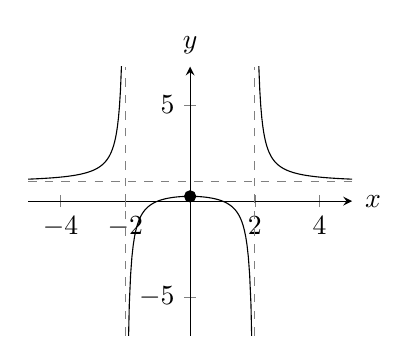
\begin{tikzpicture}
		\begin{axis}[
			scale = 0.6,
			axis x line = middle,
			axis y line = middle,
			xmin = -5,
			xmax = 5,
			ymin = -7,
			ymax = 7,
			xlabel = $x$,
			ylabel = $y$,
			%xtick = {-3, -1, 1, 3},
			%ytick = {-3, 3},
			every axis x label/.style = {
				at = {(ticklabel* cs:1.01)},
				anchor = west,
			},
			every axis y label/.style = {
				at = {(ticklabel* cs:1.01)},
				anchor = south,
			},
			restrict y to domain = -10:10
			]
			\addplot[
			black,
			samples = 100,
			domain = -5:-2
			]{(x^2-1)/(x^2-4)};
			\addplot[
			black,
			samples = 100,
			domain = -2:2
			]{(x^2-1)/(x^2-4)};
			\addplot[
			black,
			samples = 100,
			domain = 2:5
			]{(x^2-1)/(x^2-4)};
			\addplot[
			gray,
			dashed
			] coordinates {(-5, 1) (5, 1)};
			\addplot[
			gray,
			dashed
			] coordinates {(2, -7) (2, 7)};
			\addplot[
			gray,
			dashed
			] coordinates {(-2, -7) (-2, 7)};
			\addplot[mark=*] coordinates {(0, 0.25)};
		\end{axis}
	\end{tikzpicture}
	\caption{Plot of $\displaystyle f(x) = \frac{x^2 - 1}{x^2 - 4}$.}
	\label{lec7:sketch1}
\end{figure}

\noindent
Let's now tackle a rather more difficult function to sketch.

\begin{example}
	Sketch the graph of $y = x e^{-x^2 / 2}$.

	We compute the first two derivatives:
	\[
		y' = x e^{-x^2 / 2} \cdot (-x) + e^{-x^2 / 2} = (1 - x^2) e^{-x^2 / 2},
	\]
	and
	\begin{align*}
		y'' & = (1 - x^2) e^{-x^2 / 2} \cdot (-x) + e^{-x^2 / 2} \cdot (-2x) \\
		    & = -x (1 - x^2 + 2) e^{-x^2 / 2} = x (x^2 - 3) e^{-x^2 / 2}.
	\end{align*}

	\noindent
	Thus from $y$ itself we know that the domain is all of $\R$.
	We have a horizontal asymptote at $y = 0$ since
	\[
		\lim_{x \to \pm \infty} x e^{- x^2 / 2} = \lim_{t \to \infty} \sqrt{2t} e^{-t} = 0,
	\]
	wherein we did the change of variable $t = x^2 / 2$.

	Moreover $y$ is odd, since $y(-x) = -y(x)$, so it is symmetric about the origin.
	It also goes through the origin since $y(0) = 0$.

	From $y'$ we know that there are critical points at $x = \pm 1$.

	Finally from $y''$ we observe that $y''(0) = y''(\sqrt{3}) = y''(-\sqrt{3}) = 0$.

	Let us study the signs of the derivatives around these points:

	\bigskip

	\begin{adjustbox}{center}
		\begin{tabular}{r | *{11}{c}}
			$x$       &            & $-\sqrt{3}$ &            & $-1$ &            & $0$        &            & $1$ &            & $\sqrt{3}$ &            \\ \hline
			$y'$      & $-$        &             & $-$        & $0$  & $+$        &            & $+$        & $0$ & $-$        &            & $-$        \\
			$y''$     & $-$        & $0$         & $+$        & $+$  & $+$        & $0$        & $-$        & $-$ & $-$        & $0$        & $+$        \\
			$y$       & $\searrow$ &             & $\searrow$ & min  & $\nearrow$ &            & $\nearrow$ & max & $\searrow$ &            & $\searrow$ \\
			Concavity & $\frown$   & Inflection  & $\smile$   &      & $\smile$   & Inflection & $\frown$   &     & $\frown$   & Inflection & $\smile$
		\end{tabular}
	\end{adjustbox}

	\noindent
	With this at our disposal we are able to sketch the function in Figure.
\end{example}

\begin{figure}[b!]
	\centering
	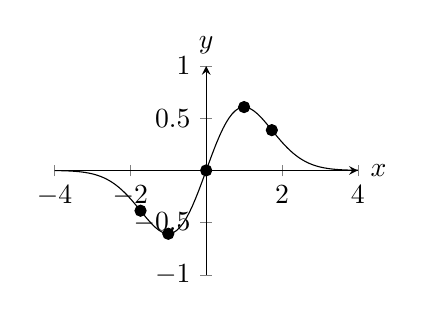
\begin{tikzpicture}
		\begin{axis}[
			scale = 0.6,
			xscale = 1,
			axis x line = middle,
			axis y line = middle,
			xmin = -4,
			xmax = 4,
			ymin = -1,
			ymax = 1,
			xlabel = $x$,
			ylabel = $y$,
			%xtick = {-3, -1, 1, 3},
			%ytick = {-3, 3},
			every axis x label/.style = {
				at = {(ticklabel* cs:1.01)},
				anchor = west,
			},
			every axis y label/.style = {
				at = {(ticklabel* cs:1.01)},
				anchor = south,
			},
			restrict y to domain = -10:10,
			height = 6cm,
			width = 8cm
			]
			\addplot[
			black,
			samples = 100,
			domain = -4:4
			]{x*exp(-x^2/2)};
			\addplot[mark=*] coordinates {(0, 0)};
			\addplot[mark=*] coordinates {(1, 0.607)};
			\addplot[mark=*] coordinates {(-1, -0.607)};
			\addplot[mark=*] coordinates {(1.732, 0.386)};
			\addplot[mark=*] coordinates {(-1.732, -0.386)};
		\end{axis}
	\end{tikzpicture}
	\caption{Plot of $y = x e^{-x^2 / 2}$.}
	\label{lec7:sketch2}
\end{figure}



\lecture[February 13, 2017]{Overdue Proofs and Antiderivatives}

\topic{Proofs of Max-min and Intermediate Value Theorem}

A long time ago (all the way back in Lecture \ref{lec3:continuity}) we stated the Max-min theorem and the Intermediate value theorem, but we did not prove them. We will now, though note that strictly speaking this is not a part of this course.

We will need to remember the definitions of limit, continuity at a point, and what we meant by a function being continuous on an interval.

As suggested back then, part of the mystery behind the proofs has to do with upper bounds of sets of real numbers.

\begin{definition}
	A number $u$ is said to be an \keyword{upper bound}\index{upper bound} for a nonempty set $S$ if $x \leq u$ for all $x \in S$.

	The number $u^*$ is called the \keyword{least upper bound}\index{least upper bound|see {supremum}} or \keyword{supremum}\index{supremum} of $S$ if $u^*$ is an upper bound for $S$ and $u^* \leq u$ for every upper bound $u$ of $S$. It is denoted $u^* = \sup(S)$.

	Similarly $\ell$ is a \keyword{lower bound}\index{lower bound} of $S$ if $\ell \leq x$ for all $x \in S$ and $\ell^* = \inf(S)$ is the \keyword{greatest lower bound}\index{greatest lower bound|see {infimum}} or \keyword{infimum}\index{infimum} of $S$ is $\ell \leq \ell^*$ for all lower bounds $\ell$ of $S$.
\end{definition}

\begin{example}
	Let $S_1 = [2, 3]$. Any $u \geq 3$ is an upper bound for $S_1$, with $\sup(S_1) = 3$.

	On the other hand, $S_2 = {]{2, \infty}[}$ has no upper bound, but many lower bounds ($\ell \leq 2$), and $\inf(S_2) = 2$.
\end{example}

\noindent
An incredibly important property of the real numbers is called \keyword{completeness}\index{completeness}. Roughly speaking this means that there are no gaps on the real number line (unlike e.g. $\Q$). In the language of of $\sup$ and $\inf$:
\begin{enumerate}
	\item A nonempty set of real numbers that has an upper bound must have a least upper bound that is a real number.
	\item A nonempty set of real numbers that has a lower bound must have a greatest lower bound that is a real number.
\end{enumerate}

\noindent
It is the last part that is the crucial difference between, for instance, $\Q$ and $\R$. Consider for example the set of all rational numbers whose square is less than or equal to 2, that is $\Set{x \in \Q \given x^2 \leq 2}$. This set certainly has an upper bound (take any $u \geq \sqrt{2}$, but it has no \emph{least} upper bound \emph{within} $\Q$ itself, since $\sqrt{2}$ isn't a rational number!

This property, called the \keyword{supremum property}, of the real numbers is (to us in this course) an \keyword{axiom}. That is to say, it cannot be proven, instead it is something we \emph{decide} to be true about the reals. (If we have a way of actually construction, of building the real numbers, then it becomes a theorem that one proves.)

This allows us to prove several interesting results.

\begin{theorem}
	If $x_1, x_2, \ldots, x_n, x_{n + 1}, \ldots$ is an increasing sequence that is bounded above;
	\[
		x_{n + 1} \geq x_n \qquad \text{and} \qquad x_n \leq K
	\]
	for some $K$ and all $n = 1, 2, 3, \ldots$, then
	\[
		\lim_{n \to \infty} x_n = L
	\]
	exists.
\end{theorem}

\noindent
The same theorem is true for decreasing sequences bounded below.

\begin{proof}
	The set $S = \Set{x_n \given n = 1, 2, 3, \ldots}$ has an upper bound $K$ by assumption, therefore by the Supremum property there exists a least upper bound $L = \sup(S)$.

	For every $\varepsilon > 0$, there exists some $N$ such that $x_N > L - \varepsilon$, because otherwise $L - \varepsilon$ would be an upper bound for $S$ that is smaller than the least upper bound $L$.

	If $n \geq N$, then $L - \varepsilon < x_N \leq x_n \leq L$, whereby $\abs{x_n - L} < \varepsilon$, so
	\[
		\lim_{n \to \infty} x_n = L. \qedhere
	\]
\end{proof}

\noindent
We will now prove some theorems we already established for functions, but this time for sequences.

\begin{theorem}\label{lec9:seqbound}
	If $a \leq x_n \leq b$ for all $n = 1, 2, 3, \ldots$, and $\lim\limits_{n \to \infty} x_L = L$, then $a \leq L \leq b$.
\end{theorem}

\begin{proof}
	Suppose $L > b$ and let $\varepsilon = L - b$. Since
	\[
		\lim_{n \to \infty} x_n = L
	\]
	there exists an $n$ such that $\abs{x_n - L} < \varepsilon$. Therefore $x_n > L - \varepsilon = L - (L - b) = b$, so $x_n > b$, a contradiction. Therefore $L \leq b$.

	Similarly for $L \geq a$.
\end{proof}

\begin{theorem}\label{lec9:seqlim}
	If $f$ is continuous on $[a, b]$, if $a \leq x_n \leq b$ for all $n = 1, 2, 3, \ldots$, and if $\lim\limits_{n \to \infty} x_n = L$, then
	\[
		\lim_{n \to \infty} f(x_n) = f(L).
	\]
\end{theorem}

\begin{proof}
	Similar to the limits of compositions of continuous functions.
\end{proof}

\noindent
These are the tools we require to prove the main result behind the two theorems we are after.

\begin{theorem}
	If $f$ is continuous on $[a, b]$, then $f$ is bounded there (i.e there exists some $K$ such that $\abs{f(x)} \leq K$ for all $x \in [a, b]$).
\end{theorem}

\begin{proof}
	We show boundedness from above.

	For each positive integer $n$, let
	\[
		S_n = \Set{x \in [a, b] \given f(x) > n}.
	\]
	Note that this is the set of $x$ values that makes this happen.

	We would like to show that $S_n$ is empty for some $n$. It would follow that $f(x) \leq n$ for this $n$, so $n$ would be an upper bound.

	Suppose $S_n$ is nonempty for all $n$. For each $n = 1, 2, 3, \ldots$, since $S_n$ is bounded below ($a$ is a lower bound by construction), by the Supremum axiom there exists a greatest lower bound, call it $x_n$.

	Since $f(x) > n$ at some point in $[a, b]$, and continuous at that point, $f(x) > n$ on some interval contained in $[a, b]$. Thus $x_n < b$ and $f(x_n) \geq n$ (otherwise by continuity $f(x) < n$ for some distance to the right of $x_n$ and $x_n$ could not be $\inf(S_n)$).

	For each $n$, $S_{n + 1} \subseteq S_n$ implies that $x_{n + 1} \geq x_n$, so $x_1, x_2, \ldots, x_n, \ldots$ is an increasing sequence bounded above by $b$, meaning that it converges to, say,
	\[
		\lim_{n \to \infty} x_n = L.
	\]

	\noindent
	By Theorem \ref{lec9:seqbound} we have $a \leq L \leq b$, and $f$ is continuous at $L$ so
	\[
		\lim_{n \to \infty} f(x_n) = f(L)
	\]
	exists by Theorem \ref{lec9:seqlim}. But since $f(x_n) \geq n$ for every $n$,
	\[
		\lim_{n \to \infty} f(x_n)
	\]
	cannot exist, since it grows arbitrarily large, so we have a contradiction. Therefore our assumption of $S_n$ always being nonempty is wrong, ergo there exists some $n$ such that $S_n$ is empty, whereby $f$ is bounded above on $[a, b]$.

	For boundedness below do almost the same thing.
\end{proof}

\noindent
We are now able to prove the Max-min theorem and the Intermediate value theorem.

\begin{theorem}[Max-min theorem]
	If $f$ is continuous on $[a, b]$, then there exists some $u, v \in [a, b]$ such that $f(v) \leq f(x) \leq f(u)$ for all $x \in [a, b]$.
\end{theorem}

\begin{proof}
	By the previous theorem, $S = \Set{f(x) \given x \in [a, b]}$ has an upper bound and by the Supremum axiom it also has a least upper bound, call it $M = \sup(S)$. Suppose there is no $u \in [a, b]$ such that $f(u) = M$. Then $1 / (M - f(x))$ is continuous on $[a, b]$ so again by the last theorem there exists some $K$ such that $1 / (M - f(x)) \leq K$ for all $x \in [a, b]$.

	By rearranging, this implies that
	\[
		f(x) \leq M - \frac{1}{K},
	\]
	which contradicts $M$ being the \emph{least} upper bound for $S$, therefore there must exist some $u \in [a, b]$ such that $f(x) \leq f(u) = M$.

	The existence of $v$ is similar.
\end{proof}

\begin{theorem}[Intermediate value theorem]
	If $f$ is continuous on $[a, b]$ and $s$ is a number between $f(a)$ and $f(b)$, then there exists some $c \in [a, b]$ such that $f(c) = s$.
\end{theorem}

\begin{proof}
	Assume $f(a) < s < f(b)$ (the other case, where $f(b) < s < f(a)$ is treated in almost the same way) and let $S = \Set{x \in [a, b] \given f(x) \leq s}$.

	The set $S$ is nonempty (at the very least it contains $a$) and bounded above ($b$ is an upper bound), so by the Supremum axiom there exists a least upper bound $\sup(S) = c$.

	Now suppose $f(c) > s$. Then $c \neq a$ and by continuity $f(x) > s$ on some interval ${]{c - \delta, c}]}$, with $\delta > 0$. But this says that $c - \delta < c$ is an upper bound for $S$, so $c$ wasn't the \emph{least} upper bound, which is a contradiction, meaning that instead we must have $f(c) \leq s$.

	We then perform the same argument to achieve $f(c) \geq s$, meaning that $f(c) = s$.
\end{proof}

\topic{Antiderivatives}

So far we have studied the problem of finding the derivative $f'$ given a function $f$. The reverse problem, finding $f$ given a derivative $f'$, is also interesting and important!

\begin{definition}[Antiderivative]
	An \keyword{antiderivative}\index{antiderivative} of a function $f$ on an interval $I$ is another function $F$ satisfying
	\[
		F'(x) = f(x)
	\]
	for all $x$ in $I$.
\end{definition}

\begin{example}
	The function $F(x) = x$ is an antiderivative to $f(x) = 1$ on any interval since $F'(x) = 1 = f(x)$ everywhere.

	Similarly, $G(x) = -1/x$ is an antiderivative to $g(x) = 1/x^2$ and $H(x) = e^{2x} + 17$ is an one for $h(x) = 2 e^{2 x}$.
\end{example}

\noindent
The last example is meant to exemplify that antiderivatives aren't unique; since all constants have derivative $0$, we can always add one and get the same derivative.

More importantly, \emph{all} antiderivatives of $f$ on an interval $I$ can be obtained by adding constants to \emph{any particular} antiderivative.

The proof of this is easy; if $F$ and $G$ are two antiderivatives to $f$ on $I$, then
\[
	\frac{d}{d x} (F(x) - G(x)) = f(x) - f(x) = 0,
\]
whereby $F(x) - G(x) = C$, with $C$ constant.

\topic{Indefinite Integrals}

The \emph{general} antiderivative of a function $f$ on an interval $I$ is $F(x) + C$, for all constants $C$, where $F$ is any particular antiderivative of $f$ on $I$.

\begin{definition}[Indefinite integral]
	The \keyword{indefinite integral}\index{integral!indefinite} of $f$ on an interval $I$ is
	\[
		\int f(x) \, d x = F(x) + C,
	\]
	for all $C \in \R$, provided $F'(x) = f(x)$ for all $x \in I$.
\end{definition}

\noindent
We already know how to compute many indefinite integrals.

\begin{examples}
	We have, amongst others,
	\[
		\int \, d x = \int 1 \, d x = x + C \quad \text{and} \quad \int x^\alpha \, d x = \frac{x^{\alpha + 1}}{\alpha + 1} + C,
	\]
	if $\alpha \neq -1$, with
	\[
		\int x^{-1} \, d x = \int \frac{1}{x} \, d x = \ln(x) + C,
	\]
	if $x > 0$.

	We have the special result
	\[
		\int e^x \, d x = e^x + C.
	\]

	\noindent
	We also know about some trigonometric results, e.g.
	\[
		\int \sin(x) \, d x = - \cos(x) + C \quad \text{and} \quad \int (\sec(x))^2 \, d x = \tan(x) + C.
	\]

	\noindent
	We can even compute some pretty complicated indefinite integrals if we just take some care. Consider, for instance,
	\[
		\int \frac{\ln(x)}{x} \, d x.
	\]

	\noindent
	If we see this as a product of $1/x$ and $\ln(x)$, we might, if we're trying to guess what this is the derivative of, come to think of the product rule, since
	\[
		\frac{d}{d x} \ln(x) \ln(x) = \frac{2 \ln(x)}{x},
	\]
	so the above indefinite integral must be $(\ln(x))^2 / 2 + C$.
\end{examples}

\noindent
Since the graphs of an indefinite integral for the various $C$ are just vertically displaced, just one of them will pass through a given point.

Thus if we know just \emph{one} point of the antiderivative some problem is looking for, we can find the right one.

\begin{example}
	Find the function $f$ the derivative of which is $f'(x) = 3 x^3 + 2 x - 3$ for all real $x$ and for which $f(1) = 0$.

	We compute the indefinite integral
	\[
		f(x) = \int 3 x^3 + 2 x - 3 \, d x = \frac{3}{4} x^4 + x^2 - 3 x + C,
	\]
	so
	\[
		f(1) = \frac{3}{4} + 1 - 3 + C = \frac{3}{4} - 2 + C = - \frac{5}{4} + C = 0,
	\]
	whereby $C = 5/4$, so $f(x) = 3/4 x^4 + x^2 - 3 x + 5/4$.
\end{example}

\noindent
This kind of problem is called an \keyword{initial-value problem}\index{initial value}, and rewriting the formulation we get
\[
	\frac{d y}{d x} = 3 x^3 + 2 x - 3,
\]
and we see that this is a differential equation.

\begin{example}
	Solve the inital-value problem
	\[
		\begin{cases}
			y' = \frac{3 + 2 x^2}{x^2} \\
			y(-2) = 1.
		\end{cases}
	\]

	\noindent
	As before we compute the indefinite integral and then insert the known information:
	\[
		y = \int \frac{3}{x^2} + 2 \, d x = - \frac{3}{x} + 2 x + C,
	\]
	so
	\[
		1 = y(-2) = \frac{3}{2} - 4 + C,
	\]
	whereby $C = 7/2$.

	This $y = -3 / x + 2 x + 7/2$ is a solution to the initial-value problem on ${]{-\infty, 0}[}$ (because this is the largest interval which contains the initial point $x = -2$ but not $x = 0$, where $y$ (and $y'$) is undefined).
\end{example}

\noindent
This, confusingly, is not really where the notion of integration comes from. Instead integration has to do with areas, but just how the indefinite integral has much to do with the derivative, so do these areas!



\lecture[February 16, 2017]{The Integral}

%!TEX root = ../lectures.tex

\topic{Areas Under Curves}

We will soon have to deal a lot with sums, usually of very many (maybe infinitely many) terms, and for this we will use sigma notation, which hopefully the student is familiar with.

\begin{figure}
	\centering
	\begin{subfigure}{0.45\textwidth}
		\centering
		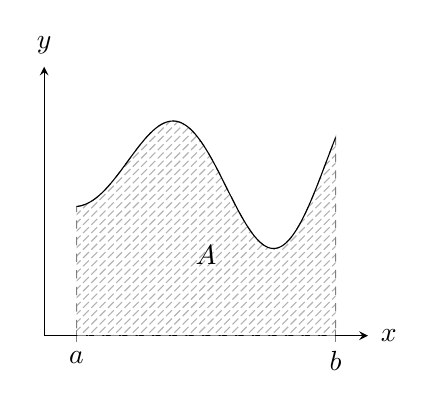
\begin{tikzpicture}
			\begin{axis}[
				scale = 0.6,
				axis x line = left,
				axis y line = left,
				xmin = 0,
				xmax = 5,
				ymin = 0,
				ymax = 10,
				xlabel = $x$,
				ylabel = $y$,
				xtick = {0.5, 4.5},
				xticklabels = {$a$, $b$},
				ytick = \empty,
				every axis x label/.style = {
					at = {(ticklabel* cs:1.01)},
					anchor = west,
				},
				every axis y label/.style = {
					at = {(ticklabel* cs:1.01)},
					anchor = south,
				},
				restrict y to domain = 0:10
				]
				\addplot[
				gray,
				dashed,
				samples = 200,
				pattern color = gray!60,
				pattern = north east lines,
				domain = 0.5:4.5
				]{0.5*(x+2)*sin((2*(x+2))r)+6} \closedcycle;
				\addplot[
				black,
				samples = 200,
				domain = 0.5:4.5
				]{0.5*(x+2)*sin((2*(x+2))r)+6};
				\addplot[mark=none] coordinates {(2.5, 3)} node{$A$};
			\end{axis}
		\end{tikzpicture}
		\caption{The precise area under some curve}
		\label{lec10:realarea}
	\end{subfigure}
	\begin{subfigure}{0.45\textwidth}
		\centering
		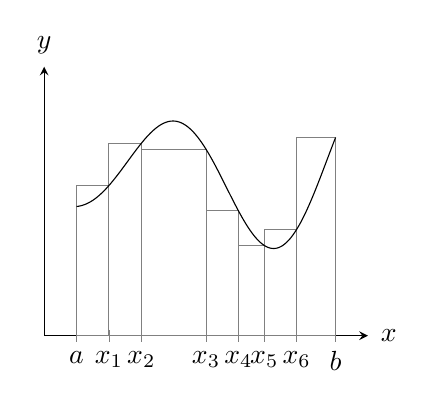
\begin{tikzpicture}
			\begin{axis}[
				scale = 0.6,
				axis x line = left,
				axis y line = left,
				xmin = 0,
				xmax = 5,
				ymin = 0,
				ymax = 10,
				xlabel = $x$,
				ylabel = $y$,
				xtick = {0.5, 1, 1.5, 2.5, 3, 3.4	, 3.9, 4.5},
				xticklabels = {$a$, $x_1$, $x_2$, $x_3$, $x_4$, $x_5$, $x_6$, $b$},
				ytick = \empty,
				every axis x label/.style = {
					at = {(ticklabel* cs:1.01)},
					anchor = west,
				},
				every axis y label/.style = {
					at = {(ticklabel* cs:1.01)},
					anchor = south,
				},
				restrict y to domain = 0:10
				]
				\addplot[
				gray,
				samples = 10,
				domain = 0.5:1
				]{5.5809} \closedcycle;
				\addplot[
				gray,
				samples = 10,
				domain = 1:1.5
				]{7.1497} \closedcycle;
				\addplot[
				gray,
				samples = 10,
				domain = 1.5:2.5
				]{6.9273} \closedcycle;
				\addplot[
				gray,
				samples = 10,
				domain = 2.5:3
				]{4.6400} \closedcycle;
				\addplot[
				gray,
				samples = 10,
				domain = 3:3.4
				]{3.3515} \closedcycle;
				\addplot[
				gray,
				samples = 10,
				domain = 3.4:3.9
				]{3.9541} \closedcycle;
				\addplot[
				gray,
				samples = 10,
				domain = 3.9:4.5
				]{7.3655} \closedcycle;
				\addplot[
				black,
				samples = 200,
				domain = 0.5:4.5
				]{0.5*(x+2)*sin((2*(x+2))r)+6};
			\end{axis}
		\end{tikzpicture}
		\caption{An approximation of the same area}
		\label{lec10:approximatearea}
	\end{subfigure}
	\caption{The area under a curve, both exact and as estimated by a sum.}
\end{figure}

Suppose we have some function $f$, and we want to find the area between $x = a$, $x = b$, the $x$-axis, and $y = f(x)$.
Now, if this region is a polygon, it's easy, but it isn't necessarily.
See, for instance, Figure \ref{lec10:realarea}.

It \emph{can} however be estimated using polygons.
We do this by \keyword{partitioning}\index{partition} (dividing) the interval $[a, b]$ into $n$ parts (not necessarily equal in length),
\[
	a = x_0 < x_1 < x_2 < \ldots < x_{n - 1} < x_n = b.
\]
Thus the smaller sections are $[x_{i - 1}, x_i]$ for all $i = 1, 2, 3, \ldots, n$.
We denote by $\Delta x_i = x_i - x_{i - 1}$ the length of these subintervals.

The point of this is that we can now approximate the area $A$ we are interested in by taking the sum of the areas of the rectangles we form as in Figure \ref{lec10:approximatearea}, namely
\[
	S_n = f(x_1) \Delta x_1 + f(x_2) \Delta x_2 + \ldots + f(x_n) \Delta x_n = \sum_{i = 1}^n f(x_i) \Delta x_i.
\]

\noindent
Of course $S_n$ is not \emph{quite} equal to $A$, since it sometimes overestimates a bit and sometimes underestimates a bit, but it seems reasonable that if we make $n$ greater, so that we're splitting the interval up into finer parts, and at the same time make sure the $\Delta x_i$ are getting smaller, then we'll approach $A$, i.e.
\[
	A = \lim_{\substack{n \to \infty \\ \max\Set{\Delta x_i} \to 0}} S_n.
\]

\begin{example}
	Find the area of the region bounded by $y = x^2$, $y = 0$, $x = 0$, and $x = b$, where $b > 0$.

	We divide the interval $[0, b]$ into $n$ equal parts, as illustrated in Figure \ref{lec10:x^2area}, each with width $\Delta x_i = b/n$.
	The height of the rectangle at $x = x_i$ is then $(i b / n)^2$, whereby\footnote{Feel free to verify on your own, perhaps by induction, that the last step is correct.}
	\[
		S_n = \sum_{i = 1}^n f(x_i) \Delta x_i = \sum_{i = 1}^n \Big ( \frac{i b}{n} \Big )^2 \frac{b}{n} = \frac{b^3}{n^3} \sum_{i = 1}^n i^2 = \frac{b^3}{n^3} \frac{n (n + 1)(2n + 1)}{6}.
	\]

	\noindent
	Taking the limit, we find that
	\[
		\lim_{n \to \infty} b^3 \frac{(n + 1)(2n + 1)}{6 n^2} = b^3 \lim_{n \to \infty} \frac{2n^2 + 3n + 1}{6 n^2} = \frac{b^3}{3} = A. \qedhere
	\]
\end{example}

\begin{figure}
	\centering
	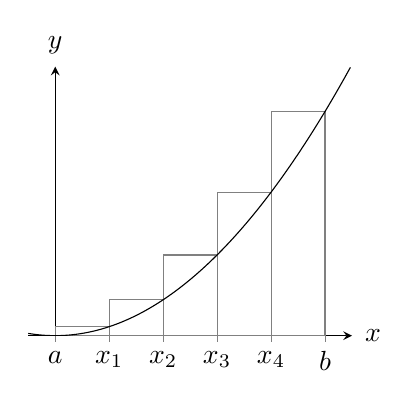
\begin{tikzpicture}
		\begin{axis}[
			scale = 0.6,
			axis x line = left,
			axis y line = middle,
			xmin = -0.5,
			xmax = 5.5,
			ymin = 0,
			ymax = 30,
			xlabel = $x$,
			ylabel = $y$,
			xtick = {0, 1, 2, 3, 4, 5},
			xticklabels = {$a$, $x_1$, $x_2$, $x_3$, $x_4$, $b$},
			ytick = \empty,
			every axis x label/.style = {
				at = {(ticklabel* cs:1.01)},
				anchor = west,
			},
			every axis y label/.style = {
				at = {(ticklabel* cs:1.01)},
				anchor = south,
			},
			restrict y to domain = 0:30
			]
			\addplot[
			gray,
			samples = 10,
			domain = 0:1
			]{1} \closedcycle;
			\addplot[
			gray,
			samples = 10,
			domain = 1:2
			]{4} \closedcycle;
			\addplot[
			gray,
			samples = 10,
			domain = 2:3
			]{9} \closedcycle;
			\addplot[
			gray,
			samples = 10,
			domain = 3:4
			]{16} \closedcycle;
			\addplot[
			gray,
			samples = 10,
			domain = 4:5
			]{25} \closedcycle;
			\addplot[
			black,
			samples = 200,
			domain = -0.5:5.5
			]{x^2};
		\end{axis}
	\end{tikzpicture}
	\caption{Estimating the area under $y = x^2$ using rectangles.}
	\label{lec10:x^2area}
\end{figure}

\noindent
We mentioned earlier that $\Delta x_i$ needn't all be equal.
Indeed, trying to use the same partition in the next problem we'd run into trouble.

\begin{exercise}
	Let $0 < a < b$, and let $k \neq -1$ be real.
	Show that the area bounded by $y = x^k$, $y = 0$, $x = a$, and $x = b$ is
	\[
		A = \frac{b^{k + 1} - a^{k + 1}}{k + 1}.
	\]

	\noindent
	Hints: Let $t = (b/a)^{1/n}$, and use the partition $x_0 = a$, $x_1 = a t$, $x_2 = a t^2$, \ldots, $x_n = a t^n = b$.

	Also recall what we know about geometric sums, i.e. that
	\[
		\sum_{i = 1}^n r^i = \frac{r^{n + 1} - 1}{r - 1},
	\]
	or maybe more useful,
	\[
		\sum_{i = 1}^n r^{i - 1} = \frac{r^n - 1}{r - 1},
	\]
	for $r \neq 1$.

	You'll also at some point change a limit to infinity to a limit at $0^+$, and use L'H\^{o}pital's rule.

	If you like, try to use the same partition as before as well, to see why this is problematic.
\end{exercise}

\topic{Definite Integrals and Riemann Sums}

In the following discussion we will assume that $f$ is continuous on the interval $[a, b]$.

Let us go back to partitions, say
\[
	P = \Set{x_0, x_1, x_2, \ldots, x_{n - 1}, x_n},
\]
such that
\[
	a = x_0 < x_1 < x_2 < \ldots < x_{n - 1} < x_n = b.
\]

\noindent
Now since $f$ is continuous on $[a, b]$, it must also be continuous on the subintervals $[x_{i - 1}, x_i]$ of $P$.
Since it is continuous on a closed interval, there must exist $\ell_i, u_i \in [x_{i - 1}, x_i]$ such that
\[
	f(\ell_i) \leq f(x) \leq f(u_i)
\]
for all $x_i \leq x \leq x_i$, by the Max-min theorem.

If we perform the same sum machinery as before with these special $\ell_i$ and $u_i$, we get areas as small and as large as possible.

\begin{definition}[Riemann sum]
	The \keyword{lower (Riemann) sum}\index{Riemann sum}\index{Riemann sum!lower}, $L(f, P)$, and the \keyword{upper (Riemann) sum}\index{Riemann sum!upper}, $U(f, P)$, for the function $f$ and the partition $P$, are
	\[
		L(f, P) = \sum_{i = 1}^n f(\ell_i) \Delta x_i, \qquad \text{and} \qquad U(f, P) = \sum_{i = 1}^n f(u_i) \Delta x_i.
	\]
\end{definition}

\begin{remark}
	If $f$ is negative, we have negative areas in our sum.
\end{remark}

\noindent
Since $L(f, P)$ is summed with the minimum for $f$ in $[x_{i - 1}, x_i]$ and $U(f, P)$ its maximum in the same interval, it is clear that
\[
	L(f, P) \leq U(f, P)
\]
for all partitions $P$.
(The only case where this might not be clear is when negative values are involved\ldots Think about it!
Draw different partitions!)

\begin{definition}[Definite integral]
	Let $f$ be a function, not necessarily continuous.
	Suppose there is exactly one number $I$ such that for \emph{every} partition $P$ of $[a, b]$ we have
	\[
		L(f, P) \leq I \leq U(f, P),
	\]
	then we say that $f$ is (Riemann) \keyword{integrable}\index{integrability} on $[a, b]$, and we call $I$ the \keyword{definite integral}\index{definite integral} of $f$ on $[a, b]$.

	We use the notation
	\[
		I = \int_a^b f(x) \, d x.
	\]

	\noindent
	Here $a$ and $b$ are called \keyword{limits of integration}, $f$ is called the \keyword{integrand}, $d x$ is called the \keyword{differential}, and $x$ is called the \keyword{variable of integration}.
\end{definition}

\noindent
Comparing this with
\[
	S_n = \sum_{i = 1}^n f(x_i) \Delta x_i,
\]
we can think of the definite integral as the sum of areas of infinitely many rectangles of height $f(x)$ and infinitesimally small widths $d x$.

We will learn next time how to efficiently calculate these sorts of quantities, but for now we close with an important theorem, the proof of which, like the Max-min theorem and the Intermediate value theorem strictly speaking doesn't belong to the course:

\begin{theorem}
	If $f$ is continuous on $[a, b]$, then $f$ is integrable on $[a, b]$.
\end{theorem}

\noindent
So far, when studying $\int\limits_a^b f(x) \, d x$, we have required $a < b$.
It turns out to be useful to drop this and allow $a = b$ and $b < a$ as well. The extension is pretty straight forward; we still have $a = x_0, x_1, \ldots, x_n = b$, but for $a = b$ they're all the same, so $\Delta x_i = 0$ (making the integral $0$), and for $b < a$ we have $\Delta x_i < 0$, so the area switches sign!

We have the following properties:

\begin{theorem}
	Let $f$ and $g$ be integrable on an interval containing $a$, $-a$, $b$, and $c$.
	Then
	\begin{romanlist}
		\item $\displaystyle \int_a^a f(x) \, d x = 0$;
		\item $\displaystyle \int_a^b f(x) \, d x = - \int_b^a f(x) \, d x$;
		\item with $A$ and $B$ constants,
		\[
			\int_a^b A f(x) + B g(x) \, d x = A \int_a^b f(x) \, d x + B \int_a^b g(x) \, d x;
		\]
		\item $\displaystyle \int_a^b f(x) \, d x + \int_b^c f(x) \, d x = \int_a^c f(x) \, d x$;
		\item if $a \leq b$, and $f(x) \leq g(x)$ for all $a \leq x \leq b$,
		\[
			\int_a^b f(x) \, d x \leq \int_a^b g(x) \, d x;
		\]
		\item (Triangle inequality), if $a \leq b$,
		\[
			\abs*{\int_a^b f(x) \, d x} \leq \int_a^b \abs{f(x)} \, d x;
		\]
		\item if $f$ is odd (i.e. $f(x) = - f(-x)$),
		\[
			\int_{-a}^a f(x) \, d x = 0;
		\]
		\item if $f$ is even  (i.e. $f(x) = f(-x)$),
		\[
			\int_{-a}^a f(x) \, d x = 2 \int_0^a f(x) \, d x.
		\]
	\end{romanlist}
\end{theorem}

\begin{proof}[(Almost literal) sketch of proof]
	\fakeitemref{1} and \fakeitemref{2} are motivated by the previous discussion.

	For \fakeitemref{3}, consider the following sketch:

	\begin{figure}[ht!]
		\centering
		\begin{subfigure}{0.3\textwidth}
			\centering
			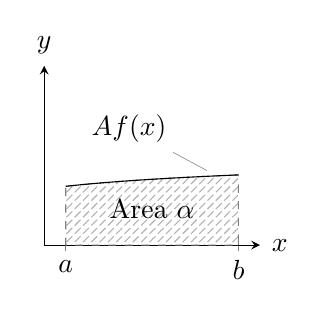
\begin{tikzpicture}
				\begin{axis}[
					scale = 0.4,
					axis x line = left,
					axis y line = left,
					xmin = 0,
					xmax = 5,
					ymin = 0,
					ymax = 15,
					xlabel = $x$,
					ylabel = $y$,
					xtick = {0.5, 4.5},
					xticklabels = {$a$, $b$},
					ytick = \empty,
					every axis x label/.style = {
						at = {(ticklabel* cs:1.01)},
						anchor = west,
					},
					every axis y label/.style = {
						at = {(ticklabel* cs:1.01)},
						anchor = south,
					},
					restrict y to domain = 0:10
					]
					\addplot[
					gray,
					dashed,
					samples = 200,
					pattern color = gray!60,
					pattern = north east lines,
					domain = 0.5:4.5
					]{ln(x+2)+4} \closedcycle;
					\addplot[
					black,
					samples = 200,
					domain = 0.5:4.5
					]{ln(x+2)+4};
					\addplot[mark=none] coordinates {(2.5, 3)} node{Area $\alpha$};
					\addplot[mark=none] coordinates {(4, 5.79176)} node[pin=150:{$A f(x)$}]{} ;
				\end{axis}
			\end{tikzpicture}
		\end{subfigure}
		\begin{subfigure}{0.3\textwidth}
			\centering
			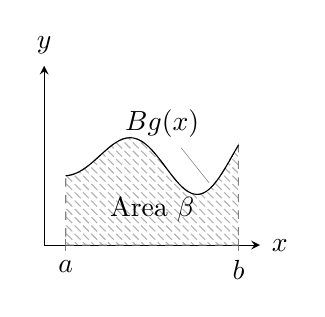
\begin{tikzpicture}
				\begin{axis}[
					scale = 0.4,
					axis x line = left,
					axis y line = left,
					xmin = 0,
					xmax = 5,
					ymin = 0,
					ymax = 15,
					xlabel = $x$,
					ylabel = $y$,
					xtick = {0.5, 4.5},
					xticklabels = {$a$, $b$},
					ytick = \empty,
					every axis x label/.style = {
						at = {(ticklabel* cs:1.01)},
						anchor = west,
					},
					every axis y label/.style = {
						at = {(ticklabel* cs:1.01)},
						anchor = south,
					},
					restrict y to domain = 0:10
					]
					\addplot[
					gray,
					dashed,
					samples = 200,
					pattern color = gray!60,
					pattern = north west lines,
					domain = 0.5:4.5
					]{0.5*(x+2)*sin((2*(x+2))r)+7} \closedcycle;
					\addplot[
					black,
					samples = 200,
					domain = 0.5:4.5
					]{0.5*(x+2)*sin((2*(x+2))r)+7};
					\addplot[mark=none] coordinates {(2.5, 3)} node{Area $\beta$};
					\addplot[mark=none] coordinates {(4, 4.39028)} node[pin=100:{$B g(x)$}]{} ;
				\end{axis}
			\end{tikzpicture}
		\end{subfigure}
		\begin{subfigure}{0.3\textwidth}
			\centering
			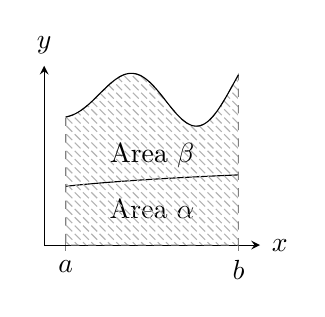
\begin{tikzpicture}
				\begin{axis}[
					scale = 0.4,
					axis x line = left,
					axis y line = left,
					xmin = 0,
					xmax = 5,
					ymin = 0,
					ymax = 15,
					xlabel = $x$,
					ylabel = $y$,
					xtick = {0.5, 4.5},
					xticklabels = {$a$, $b$},
					ytick = \empty,
					every axis x label/.style = {
						at = {(ticklabel* cs:1.01)},
						anchor = west,
					},
					every axis y label/.style = {
						at = {(ticklabel* cs:1.01)},
						anchor = south,
					},
					restrict y to domain = 0:20
					]
					\addplot[
					black,
					samples = 200,
					domain = 0.5:4.5
					]{ln(x+2)+4};
					\addplot[mark=none] coordinates {(2.5, 3)} node{Area $\alpha$};
					\addplot[
					gray,
					dashed,
					samples = 200,
					pattern color = gray!60,
					pattern = north west lines,
					domain = 0.5:4.5
					]{ln(x+2)+4+0.5*(x+2)*sin((2*(x+2))r)+7} \closedcycle;
					\addplot[
					black,
					samples = 200,
					domain = 0.5:4.5
					]{ln(x+2)+4+0.5*(x+2)*sin((2*(x+2))r)+7};
					\addplot[mark=none] coordinates {(2.5, 7.5)} node{Area $\beta$};
				\end{axis}
			\end{tikzpicture}
		\end{subfigure}
	\end{figure}

	\noindent
	For \fakeitemref{4}, at least when $a \leq c \leq b$, consider this picture:

	\begin{figure}[ht!]
		\centering
		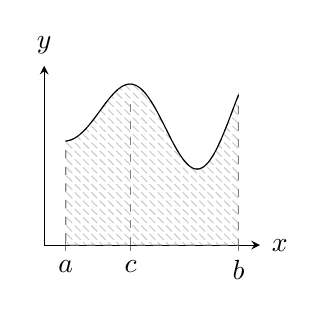
\begin{tikzpicture}
			\begin{axis}[
				scale = 0.4,
				axis x line = left,
				axis y line = left,
				xmin = 0,
				xmax = 5,
				ymin = 0,
				ymax = 10,
				xlabel = $x$,
				ylabel = $y$,
				xtick = {0.5, 2, 4.5},
				xticklabels = {$a$, $c$, $b$},
				ytick = \empty,
				every axis x label/.style = {
					at = {(ticklabel* cs:1.01)},
					anchor = west,
				},
				every axis y label/.style = {
					at = {(ticklabel* cs:1.01)},
					anchor = south,
				},
				restrict y to domain = 0:20
				]
				\addplot[
				gray,
				dashed,
				samples = 200,
				pattern color = gray!40,
				pattern = north west lines,
				domain = 0.5:4.5
				]{0.5*(x+2)*sin((2*(x+2))r)+7} \closedcycle;
				\addplot[
				black,
				samples = 200,
				domain = 0.5:4.5
				]{0.5*(x+2)*sin((2*(x+2))r)+7};
				\addplot[
				gray,
				dashed
				] coordinates {(2, 0) (2, 7.97872)};
			\end{axis}
		\end{tikzpicture}
	\end{figure}

	\noindent
	If is isn't true that $a \leq c \leq b$, consider rearranging the same picture, and now some of the integrals will be negative because of the order of the limits of integration.

	\fakeitemref{5} is probably obvious.
	If not, consider the Riemann sums; since $f$ is bounded by $g$, so must the heights in the sums.

	\fakeitemref{6} is just \fakeitemref{5}, since $-\abs{f(x)} \leq f(x) \leq \abs{f(x)}$.
	The only remaining mystery is to prove that $\abs{f}$ must be integrable on $[a, b]$ when $f$ is (which is in fact true).

	For \fakeitemref{7} and \fakeitemref{8}, draw the appropriately symmetric pictures!
\end{proof}

\noindent
Using these properties and remembering that fundamentally they represent areas we can sometimes reduce definite integral problems to very, very simple computations.

\begin{examples}
	Calculate
	\[
		\int_{-2}^2 2 + 5 x \, d x, \qquad \int_0^3 2 + x \, d x, \qquad \text{and} \qquad \int_{-3}^3 \sqrt{9 - x^2} \, d x.
	\]

	\noindent
	We use the linearity of the integral, meaning that
	\[
		\int_{-2}^2 2 + 5 x \, d x = \int_{-2}^2 2 \, d x + \int_{-2}^2 5 x \, d x.
	\]
	The first integral in the right-hand side is just the area of a rectangle of height $2$ and width $4$, so it is $8$.
	The second integral is the integral of an odd function over a symmetric interval, whereby it is $0$, so
	\[
		\int_{-2}^2 2 + 5 x \, d x = 8 + 0 = 8.
	\]

	\noindent
	For the second one, sketch the graph and we notice that the area we're interested in is just a trapezoid, consisting of one rectangle of height 2 and width 3, on top of which is a triangle of height 3 and base 3, so
	\[
		\int_0^3 2 + x \, d x = 3 \cdot 2 + \frac{1}{2} \cdot 3 \cdot 3 = \frac{21}{2}.
	\]

	\noindent
	For the third and final one we recognise that the integrand $\sqrt{9 - x^2}$ is the expression for the upper half of a circle centred on the origin with radius 3.
	Therefore
	\[
		\int_{-3}^3 \sqrt{9 - x^2} \, d x = \frac{1}{2} \cdot \pi \cdot 3^2 = \frac{9 \pi}{2}. \qedhere
	\]
\end{examples}



\lecture[February 20, 2017]{The Fundamental Theorem of Calculus}

%!TEX root = ../lectures.tex

\topic{Mean-Value Theorem for Integrals}

Just like the derivative, definite integrals have a mean-value property.

\begin{theorem}[Mean-value theorem for integrals]\index{mean-value theorem!integrals}
	If $f$ is continuous on $\interval{a}{b}$, then there exists a point $c \in \interval{a}{b}$ such that
	\[
		\int_a^b f(x) \, d x = (b - a) f(c).
	\]
\end{theorem}

\begin{proof}
	Since $f$ is continuous on $\interval{a}{b}$, and $\interval{a}{b}$ is a closed and finite interval, we know by the Max-min theorem that there exist $\ell, u \in \interval{a}{b}$ such that
	\[
		m = f(\ell) \leq f(x) \leq f(u) = M
	\]
	for all $a \leq x \leq b$.

	Now consider the very simple partition $P_1$ of $\interval{a}{b}$ with $a = x_0 < x_1 = b$.
	Then
	\[
		m (b - a) = L(f, P_1) \leq \int_a^b f(x) \, d x \leq U(f, P_1) = M(b - a).
	\]

	\noindent
	Thus
	\[
		f(\ell) = m \leq \frac{1}{b - a} \int_a^b f(x) \, d x \leq M = f(u).
	\]

	\noindent
	By the Intermediate value theorem, $f(x)$ attains every value between $f(\ell)$ and $f(u)$, so there exists some $c$ between $\ell$ and $u$ such that
	\[
		f(c) = \frac{1}{b - a} \int_a^b f(x) \, d x \quad \Longleftrightarrow \quad \int_a^b f(x) \, d x = (b - a) f(c). \qedhere
	\]
\end{proof}

\begin{figure}
	\centering
	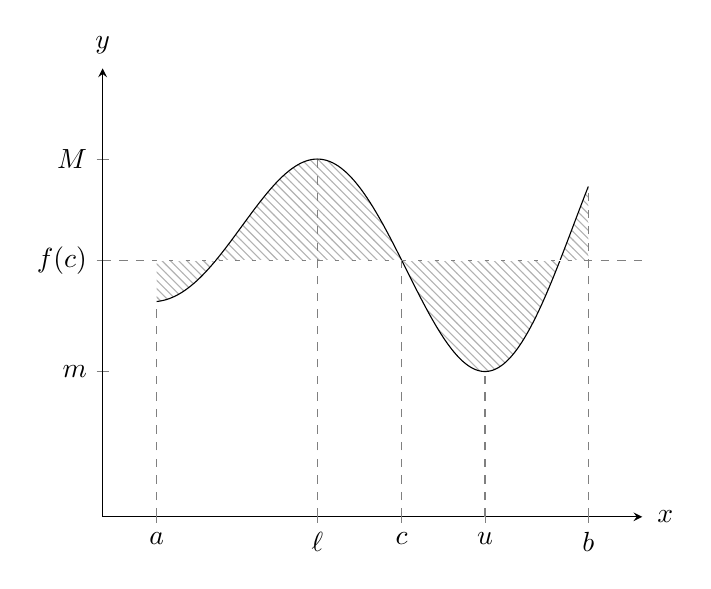
\begin{tikzpicture}
		\begin{axis}[
			scale = 1,
			axis x line = middle,
			axis y line = middle,
			xmin = 0,
			xmax = 5,
			ymin = 0,
			ymax = 10,
			xlabel = $x$,
			ylabel = $y$,
			xtick = {0.5, 1.98933, 2.77147, 3.54277, 4.5},
			xticklabels = {$a$, $\ell$, $c$, $u$, $b$},
			ytick = {3.23982, 5.7188, 7.97918},
			yticklabels = {$m$, $f(c)$, $M$},
			every axis x label/.style = {
				at = {(ticklabel* cs:1.01)},
				anchor = west,
			},
			every axis y label/.style = {
				at = {(ticklabel* cs:1.01)},
				anchor = south,
			},
			restrict y to domain = 0:20
			]
			\addplot[
			name path = F,
			black,
			samples = 200,
			domain = 0.5:4.5
			]{0.5*(x+2)*sin((2*(x+2))r)+6};
			\addplot[
			gray,
			dashed
			] coordinates {(0.5, 0) (0.5, 4.80134)};
			\addplot[
			gray,
			dashed
			] coordinates {(1.98933, 0) (1.98933, 7.97918)};
			\addplot[
			gray,
			dashed
			] coordinates {(2.77147, 0) (2.77147, 5.7188)};
			\addplot[
			gray,
			dashed
			] coordinates {(3.54277, 0) (3.54277, 3.23982)};
			\addplot[
			gray,
			dashed
			] coordinates {(4.5, 0) (4.5, 7.36554)};
			\addplot[
			gray,
			dashed
			] coordinates {(0, 5.7188) (5, 5.7188)};
			\addplot[
			name path = G,
			gray!0,
			dashed,
			domain = 0.5:4.5
			]{5.7188};
			\addplot[
			pattern color = gray!60,
			pattern = north west lines
			] fill between [of = F and G];
		\end{axis}
	\end{tikzpicture}
	\caption{Visualisation of the Mean-value theorem for integrals.}
	\label{lec10:meanvalints}
\end{figure}

This value
\[
	\bar{f} = \frac{1}{b - a} \int_a^b f(x) \, d x
\]
is often called the \keyword{average value}\index{function!average value} or \keyword{mean value} of $f$ on $\interval{a}{b}$.
This is because the area under $f(c)$ and above $f(x)$ is the same as the area above $f(c)$ and below $f(x)$.
To verify this, try computing $\int_a^b f(x) - \bar{f} \, d x$.

\topic{Piecewise Continuous Functions}

Sometimes we will want to integrate functions that aren't continuous.
An important class of such functions are \keyword{piecewise continuous}\index{piecewise continuity} functions.

\begin{figure}[b!]
	\centering
	\begin{tikzpicture}
		\begin{axis}[
			scale = 1,
			axis x line = middle,
			axis y line = middle,
			xmin = 0,
			xmax = 5,
			ymin = 0,
			ymax = 10,
			xlabel = $x$,
			ylabel = $y$,
			xtick = {0.5, 1.5, 3, 4.5},
			xticklabels = {$a$, $c_1$, $c_2$, $b$},
			ytick = \empty,
			every axis x label/.style = {
				at = {(ticklabel* cs:1.01)},
				anchor = west,
			},
			every axis y label/.style = {
				at = {(ticklabel* cs:1.01)},
				anchor = south,
			},
			restrict y to domain = 0:20
			]
			\addplot[
			black,
			samples = 200,
			domain = 0.5:1.5
			]{exp(-x)+4};
			\addplot[
			black,
			samples = 200,
			domain = 1.5:3
			]{0.5*(x+2)*sin((2*(x+2))r)+6};
			\addplot[
			black,
			samples = 200,
			domain = 3:4.5
			]{ln(x)+2};
			\addplot[mark=*] coordinates {(0.5, 4.60653)};
			\addplot[mark=*] coordinates {(1.5, 4.22313)};
			\addplot[mark=o] coordinates {(1.5, 7.14973)};
			\addplot[mark=o] coordinates {(3, 4.63995)};
			\addplot[mark=*] coordinates {(3, 3.5)};
			\addplot[mark=o] coordinates {(3, 3.09861)};
			\addplot[mark=*] coordinates {(4.5, 3.50408)};
			\addplot[
			dashed,
			gray
			] coordinates {(0.5, 0) (0.5, 4.60653)};
			\addplot[
			dashed,
			gray
			] coordinates {(1.5, 0) (1.5, 7.14973)};
			\addplot[
			dashed,
			gray
			] coordinates {(3, 0) (3, 4.63995)};
			\addplot[
			dashed,
			gray
			] coordinates {(4.5, 0) (4.5, 3.50408)};
		\end{axis}
	\end{tikzpicture}
	\caption{An example of a piecewise continuous function.}
	\label{lec10:piecewisecontinuous}
\end{figure}

See for instance Figure \ref{lec10:piecewisecontinuous}.
Clearly this function isn't continuous, but equally clearly there is an area underneath it.

\begin{definition}[Piecewise continuous function]
	Let $c_0 < c_1 < c_2 < \ldots < c_n$ be a \emph{finite} set of points.
	A function $f$ defined on $\interval{c_0}{c_n}$, except possibly at some of the $c_i$, for $0 \leq i \leq n$, is called \keyword{piecewise continuous} on the interval if for each $1 \leq i \leq n$ there exists a function $F_i$ continuous on the closed interval $\interval{c_{i-1}}{c_i}$ such that $f(x) = F_i(x)$ on $\interval[open]{c_{i-1}}{c_i}$.

	In this case we \emph{define} the definite integral of $f$ from $c_0$ to $c_n$ to be
	\[
		\int_{c_0}^{c_n} f(x) \, d x = \sum_{i = 1}^n \int_{c_{i - 1}}^{c_i} F_i(x) \, d x.
	\]
\end{definition}

\topic{The Fundamental Theorem of Calculus}

There is an important relation between definite integrals and indefinite integrals.
Recall how we defined $\ln(x)$ as a particular area under $1/t$, and as a consequence we found that $\frac{d}{d x} \ln(x) = 1/x$.

This is no coincidence, and is a special case of the following theorem:

\begin{theorem}[Fundamental Theorem of Calculus]\index{fundamental theorem of calculus}
	Suppose that $f$ is continuous on the interval $I$ containing the point $a$.

	\subsubsection*{Part I}

	Let $F$ be the function defined by
	\[
		F(x) = \int_a^x f(t) \, d t.
	\]
	Then $F$ is differentiable on $I$ and $F'(x) = f(x)$ there.

	Therefore $F$ is an antiderivative of $f$ on $I$, i.e.
	\[
		\frac{d}{d x} \int_a^x f(t) \, d t = f(x).
	\]

	\subsubsection*{Part II}

	If $G$ is \emph{any} antiderivative of $f$ on $I$, so that $G'(x) = f(x)$ on $I$, then for any $b$ in $I$ we have
	\[
		\int_a^b f(x) \, d x = G(b) - G(a).
	\]
\end{theorem}

\begin{proof}
	The proof of Part I boils down to the definition of the derivative:
	\begin{align*}
		F'(x) & = \lim_{h \to 0} \frac{F(x + h) - F(x)}{h} = \lim_{h \to 0} \frac{1}{h} \Big ( \int_a^{x + h} f(t) \, d t - \int_a^x f(t) \, d t \Big ) \\
		      & = \lim_{h \to 0} \frac{1}{h} \int_x^{x + h} f(t) \, d t,
	\end{align*}
	which by the Mean-value theorem for integrals is equal to
	\[
		\lim_{h \to 0} \frac{1}{h} \cdot h \cdot f(c) = \lim_{h \to 0} f(c)
	\]
	for some $c \in \interval{x}{x+h}$, with $c$ depending on $h$.
	Now as $h \to 0$, clearly $c$ being squeezed between $x$ and $x + h$ forces $c$ to approach $x$, so this is in turn equal to
	\[
		\lim_{c \to x} f(c) = f(x),
	\]
	since $f$ is continuous.

	For Part II, if $G'(x) = f(x)$, then $F(x) = G(x) + C$ (since they're both antiderivatives they must differ by a constant).
	Therefore
	\[
		\int_a^x f(t) \, d t = F(x) = G(x) + C.
	\]
	By taking $x = a$ we get
	\[
		\int_a^a f(t) \, d t = 0 = F(a) = G(a) + C,
	\]
	so $C = - G(a)$.

	Now instead take $x = b$, and we get
	\[
		\int_a^b f(t) \, d t = F(b) = G(b) + C = G(b) - G(a). \qedhere
	\]
\end{proof}

\noindent
Both of these are very useful.
The first part tells us how to differentiate a definite integral with respect of its upper limit, and the second part tells us how to evaluate a definite integral if you can find \emph{any} antiderivative of the integrand.

Since we will be doing this second part quite a lot, we'll introduce a new piece of notation that makes life a bit easier: we'll write
\[
	F(x) \Big \rvert_a^b = F(b) - F(a),
\]
so that, for instance,
\[
	\int_a^b f(x) \, d x = \Big ( \int f(x) \, d x \Big ) \biggr \rvert_a^b.
\]

\begin{example}
	Evaluate
	\[
		\int_0^a x^2 \, d x = \frac{1}{3} x^3 \Big \rvert_0^a = \frac{1}{3} a^3 - \frac{1}{3} 0^3 = \frac{a^3}{3}. \qedhere
	\]
\end{example}

\begin{example}
	Compute
	\begin{align*}
		\int_{-1}^2 x^2 - 3 x + 2 \, d x & = \Big ( \frac{1}{3} x^3 - \frac{3}{2} x^2 + 2 x \Big ) \biggr \rvert_{-1}^2                                                           \\
		                                 & = \frac{1}{3} \cdot 8 - \frac{3}{2} \cdot 4 + 4 - \Big ( \frac{1}{3} \cdot -1 - \frac{3}{2} \cdot 1 - 2 \Big ) = \frac{9}{2}. \qedhere
	\end{align*}
\end{example}

\begin{example}
	Find the area bounded by the $x$-axis and the curve $y = 3x - x^2$.

	First we need to find where $y = 3x - x^2$ intersects the $x$-axis: $0 = 3 x - x^2 = x (3 - x)$, so $x = 0$ and $x = 3$.
	Therefore the area is
	\[
		A = \int_0^3 3 x - x^2 \, d x = \Big ( \frac{3}{2} x^2 - \frac{1}{3} x^3 \Big ) \biggr \rvert_0^3 = \frac{27}{2} - \frac{27}{3} - (0 - 0) = \frac{27}{6} = \frac{9}{2}. \qedhere
	\]
\end{example}

\begin{example}
	Find the average value of $f(x) = e^{-x} + \cos(x)$ on the interval $\interval{-\pi/2}{0}$.

	We recall from the Mean-value theorem for integrals that what we want to compute it
	\[
		\bar{f} = \frac{1}{b - a} \int_a^b f(x) \, d x,
	\]
	so
	\begin{align*}
		\bar{f} & = \frac{1}{0 - (- \pi/2)} \int_{-\pi/2}^0 e^{-x} + \cos(x) \, d x = \frac{2}{\pi} (-e^{-x} + \sin(x)) \Big \rvert_{-\pi/2}^0 \\
		        & = \frac{2}{\pi} (-1 + 0 + e^{\pi/2} - (-1)) = \frac{2}{\pi} e^{\pi/2}. \qedhere
	\end{align*}
\end{example}

\noindent
We discuss the following example as a cautionary note.

\begin{counterexample}[Improper integral]
	We know that $\frac{d}{d x} \ln\abs{x} = 1/x$ if $x \neq 0$.
	Even so it is \keyword{incorrect} to say that
	\[
		\int_{-1}^1 \frac{d x}{x} = \ln\abs{x} \Big \rvert_{-1}^1 = 0 - 0 = 0,
	\]
	even though $1/x$ is odd.
	This is because $1/x$ is undefined at $x = 0$, so $1/x$ is not integrable on $\interval{-1}{0}$ or $\interval{0}{1}$.

	All this to say that it might sometimes be important to keep track of where one's integrand is defined.

	There are ways to deal with some of these so-called \keyword{improper integrals}\index{integral!improper}, although not this one in particular.
\end{counterexample}

\noindent
Finally we'll work through some examples that use the Fundamental theorem in interesting ways.

\begin{example}
	Differentiate
	\[
		F(x) = \int_x^3 e^{-t^2} \, d t.
	\]

	\noindent
	We note that the Fundamental theorem requires the unknown $x$ to be the upper limit of integration, so we first switch the order by negating the integrand:
	\[
		F(x) = - \int_3^x e^{-t^2} \, d t,
	\]
	so by the Fundamental theorem
	\[
		F'(x) = - e^{-x^2}. \qedhere
	\]
\end{example}

\noindent
In the following example we'll combine the Fundamental theorem with the chain rule, that is to say
\[
	\frac{d}{d x} \int_a^{g(x)} f(t) \, d t = f(g(x)) \cdot g'(x).
\]

\begin{example}
	Differentiate
	\[
		G(x) = \int_{x^2}^{x^3} e^{-t^2} \, d t.
	\]

	\noindent
	First we note that
	\[
		G(x) = \int_0^{x^3} e^{-t^2} \, d t + \int_{x^2}^0 e^{-t^2} \, d t = \int_0^{x^3} e^{-t^2} \, d t - \int_0^{x^2} e^{-t^2} \, d t,
	\]
	so
	\[
		G'(x) = e^{-(x^3)^2} \cdot (3 x^2) - e^{-(x^2)^2} \cdot (2 x) = 3x^2 e^{-x^6} - 2xe^{-x^4}. \qedhere
	\]
\end{example}



\lecture[February 23, 2017]{Method of Substitution}

\topic{Method of Substitution}

So far we have calculated all integrals pretty much by inspection, since we know quite a few derivatives, e.g.
\begin{alignat*}{2}
	  & \int x^r \, d x = \frac{x^{r + 1}}{r + 1} + C, ~r \neq -1, ~                          &   & \int \frac{1}{x} \, d x = \ln\abs{x} + C, ~x \neq 0,                                   \\
	  & \int (\sec(x))^2 \, d x = \tan(x) + C, ~                                              &   & \int \frac{1}{\sqrt{a^2 - x^2}} \, d x = \arcsin\Big ( \frac{x}{a} \Big ) + C, ~a > 0, \\
	  & \int \frac{1}{a^2 + x^2} \, d x = \frac{1}{a} \arctan\Big ( \frac{x}{a} \Big ) + C, ~ &   & \int e^{a x} \, d x = \frac{1}{a} e^{a x} + C,                                         \\
	  & \int b^{a x} \, d x = \frac{1}{a \ln(b)} b^{a x} + C, ~                               &   & \text{et cetera\ldots}
\end{alignat*}

\noindent
However this is not always enough, sometimes we need other techniques.
One of the most important ones is the \keyword{method of substitution}\index{method of substitution}, which is really just applying the integral to the chain rule.
We know that
\[
	\frac{d}{d x} f(g(x)) = f'(g(x)) \cdot g'(x),
\]
whereby
\[
	\int f'(g(x) \cdot g'(x) \, d x = f(g(x)) + C.
\]

\noindent
In the language of differentials, it looks like this:

Let $u = g(x)$.
Then $\frac{d u}{d x} = g'(x)$, which, if we treat $d u$ and $d x$ as differentials, becomes $d u = g'(x) \, d x$, which means that
\[
	\int f'(g(x)) \cdot \underbrace{g'(x) \, d x}_{=\, d u} = \int f'(u) \, d u = f(u) + C = f(g(x)) + C.
\]
(We have not spoken about differentials, and we probably aren't going to, but we may consider the above ideas as a way to remember what to do.)

\begin{example}
	Compute the integral of $x / (x^2 + 1)$.

	We let $u = x^2 + 1$, whereby $d u = 2 x \, d x$, so $x \, d x = 1/2 \, d u$.
	Therefore
	\begin{align*}
		\int \frac{x}{x^2 + 1} \, d x & = \frac{1}{2} \int \frac{d u}{u} = \frac{1}{2} \ln\abs{u} + C \\
		                              & = \frac{1}{2} \ln(x^2 + 1) + C = \ln(\sqrt{x^2 + 1}) + C.
	\end{align*}
\end{example}

\begin{example}
	Find the indefinite integral of $\sin(3 \ln(x)) / x$.

	We let $u = 3 \ln(x)$, meaning that $d u = 3 / x \, d x$.
	Therefore
	\begin{align*}
		\int \frac{\sin(3 \ln(x))}{x} \, d x & = \frac{1}{3} \int \sin(u) \, d u = - \frac{1}{3} \cos(u) + C \\
		                                     & = - \frac{1}{3} \cos(3 \ln(x)) + C. \qedhere
	\end{align*}
\end{example}

\begin{example}
	Compute the integral of $e^x \sqrt{1 + e^x}$.

	First let $u = 1 + e^x$, whereby $d u = e^x \, d x$, so that
	\[
		\int e^x \sqrt{1 + e^x} \, d x = \int \sqrt{u} \, d y = \frac{2}{3} u^{3 / 2} + C = \frac{2}{3} ( 1 + e^x )^{3 / 2} + C. \qedhere
	\]
\end{example}

\noindent
In all of these examples the substitutions required are fairly obvious.
Regrettably, life isn't always that good:

\begin{example}
	Integrate $1 / (x^2 + 4 x + 5)$.

	A very clever thing to do, which we'll formalise and make systematic in the future, is to complete the square of the denominator.
	In other words
	\[
		x^2 + 4 x + 5 = (x + 2)^2 + 1,
	\]
	so
	\[
		\int \frac{1}{x^2 + 4 x + 5} \, d x = \int \frac{d x}{(x + 2)^2 + 1}.
	\]

	\noindent
	If we now let $u = x + 2$ we get $d u = d x$, which means that
	\[
		\int \frac{d x}{(x + 2)^2 + 1} = \int \frac{d u}{u^2 + 1} = \arctan{u} + C = \arctan{x + 2} + C. \qedhere
	\]
\end{example}

\begin{example}
	Find the indefinite integral of $1 / \sqrt{e^{2 x} - 1}$.

	We first break $e^x$ out of the square root, whereby
	\[
		\int \frac{d x}{\sqrt{e^{2 x} - 1}} = \int \frac{d x}{e^x \sqrt{1 - e^{- 2x}}} = \int \frac{e^{-x}}{\sqrt{1 - (e^{- x})^2}} \, d x.
	\]

	\noindent
	By now taking $u = e^{-x}$ we have $d u = - e^{-x} \, d x$, which gives us
	\[
		\int \frac{e^{-x}}{\sqrt{1 - (e^{- x})^2}} \, d x = - \int \frac{d u}{\sqrt{1 - u^2}} = - \arcsin(u) + C = - \arcsin(e^{-x}) + C. \qedhere
	\]
\end{example}

\noindent
With this said substitution doesn't always work.
We will not be able to substitute our way through
\[
	\int x^2 (1 + x^8)^{1/3} \, d x,
\]
for instance (though we will learn a method that works for this one).

We can of course use substitution in definite integrals as well, but we need to be careful with the limits of integration.

\begin{theorem}
	Suppose $g$ is differentiable on $[a, b]$ and that $g(a) = A$ and $g(b) = B$, and suppose that $f$ is continuous on the range of $g$.
	Then
	\[
		\int_a^b f(g(x)) \cdot g'(x) \, d x = \int_A^B f(u) \, d u.
	\]
\end{theorem}

\begin{proof}
	Let $F$ be an antiderivative of $f$, then
	\[
		\frac{d}{d x} F(g(x)) = F'(g(x)) \cdot g'(x) = f(g(x)) \cdot g'(x),
	\]
	which means that
	\begin{align*}
		\int_a^b f(g(x)) \cdot g'(x) \, d x & = F(g(x)) \Big \rvert_a^b = F(g(b)) - F(g(a))                         \\
		                                    & = F(B) - F(A) = F(u) \Big \rvert_A^B = \int_A^B f(u) \, d u. \qedhere
	\end{align*}
\end{proof}

\noindent
The point being that we cannot keep the $x$-values when we are dealing with $u$-values.
Unless we switch back before evaluating!

\begin{example}
	Evaluate
	\[
		I = \int_0^8 \frac{\cos(\sqrt{x + 1})}{\sqrt{x + 1}} \, d x.
	\]

	\noindent
	Let $u = \sqrt{x + 1}$, yielding $d u = d x / (2 \sqrt{x + 1})$.
	If $x = 0$, then $u = 1$, and if $x = 8$, then $u = 3$, so
	\[
		I = 2 \int_1^3 \cos(u) \, d u = 2 \sin(u) \Big \rvert_1^3 = 2 \sin(3) - 2 \sin(1),
	\]
	or alternatively
	\[
		I = 2 \int_{x = 0}^{x = 8} \cos(u) \, d u = 2 \sin(u) \Big \rvert_{x = 0}^{x = 8} = 2 \sin(\sqrt{x + 1}) \Big \rvert_0^8 = 2 \sin(3) - 2 \sin(1). \qedhere
	\]
\end{example}

\begin{example}
	Evaluate
	\[
		I = \int_0^\pi (2 + \sin(x / 2))^2 \cos(x / 2) \, d x.
	\]

	\noindent
	We let $u = 2 + \sin(x / 2)$, meaning that $d u = \cos(x / 2) / 2 \, d x$, and if $x = 0$, $u = 0$, and if $x = \pi$, then $u = 3$.
	Thus
	\[
		I = \int_2^3 = u^2 \, d u = \frac{2}{3} u^3 \Big \rvert_2^3 = \frac{2}{3} (27 - 8) = \frac{38}{3}. \qedhere
	\]
\end{example}

\begin{remark}
	Note that $f$ being continuous on the range of $g$ is important.
	Consider
	\[
		\int_{-1}^1 x \csc(x^2) \, d x,
	\]
	with $u = x^2$ and $d u = 2 x \, d x$ it would seem as though this becomes
	\[
		\frac{1}{2} \int_1^1 \csc(u) \, d u = 0,
	\]
	but this is \keyword{incorrect}!
	Indeed $\csc$ is discontinuous at $x = 0$, and we are attempting to compute an infinite area.
	This is another example of an improper integral.
\end{remark}

\noindent
In general, if the integrand is a quotient where the numerator is (close to) the derivative of the denominator, substitution will lead us beautifully toward a logarithm.

\begin{example}
	To integrate $\tan(x)$, let $u = \cos(x)$ and $d u = - \sin(x) \, d x$, whereby
	\begin{align*}
		\int \tan(x) \, d x & = \int \frac{\sin(x)}{\cos(x)} \, d x = - \int \frac{d u}{u} = - \ln\abs{u} + C                  \\
		                    & = - \ln\abs{\cos(x)} + C = \ln\abs[\Big]{\frac{1}{\cos(x)}} + C = \ln\abs{\sec(x)} + C. \qedhere
	\end{align*}
\end{example}

\noindent
We close with another example where the substitution isn't all that obvious.

\begin{example}
	Integrate $\sqrt{1 - x^2}$ between $x = 0$ and $x = 1$.
	We let $u = \arcsin(x)$, whereby $x = \sin(u)$, and implicit differentiation $d x = \cos(u) \, d u$.
	Thus
	\begin{align*}
		\int_0^1 \sqrt{1 - x^2} \, d x & = \int_0^{\pi/2} \underbrace{\sqrt{1 - (\sin(u))^2}}_{=\, \cos(u)} \cos(u) \, d u = \int_0^{\pi/2} (\cos(u))^2 \, d u                         \\
		                               & = \int_0^{\pi/2} \frac{1}{2} + \frac{1}{2} \cos(2 u) \, d u = \frac{u}{2} \Big \rvert_0^{\pi/2} + \frac{1}{4} \sin(2 u) \Big \rvert_0^{\pi/2} \\
		                               & = \frac{\pi}{4} + \frac{1}{4} (\sin(\pi) - \sin(0)) = \frac{\pi}{4}.
	\end{align*}

	\noindent
	Note that of course we are calculating the area of the unit disc contained in the first quadrant, which by simple geometry is indeed $\pi / 4$.
\end{example}

\topic{Areas Between Curves}

Recall first of all that $\int_a^b f(x) \, d x$ measures the area between $y = f(x)$, $y = 0$, $x = a$, and $x = b$, except it treats parts under the $x$-axis as negative areas.

If, for some reason, we don't want this, it is easily avoided: simply take the absolute value of the integrand!


\begin{figure}
	\centering
	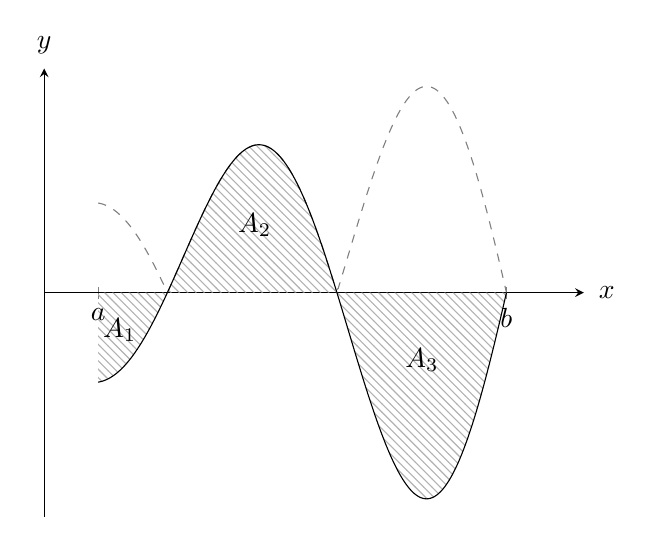
\begin{tikzpicture}
		\begin{axis}[
			scale = 1,
			axis x line = middle,
			axis y line = middle,
			xmin = 0,
			xmax = 5,
			ymin = -3,
			ymax = 3,
			xlabel = $x$,
			ylabel = $y$,
			xtick = {0.5, 4.283},
			xticklabels = {$a$, $b$},
			ytick = {3.23982, 5.7188, 7.97918},
			yticklabels = {$m$, $f(c)$, $M$},
			every axis x label/.style = {
				at = {(ticklabel* cs:1.01)},
				anchor = west,
			},
			every axis y label/.style = {
				at = {(ticklabel* cs:1.01)},
				anchor = south,
			},
			restrict y to domain = -10:10
			]
			\addplot[
			gray,
			dashed,
			samples = 200,
			domain = 0.5:4.283
			]{abs(0.5*(x+2)*sin((2*(x+2))r))};
			\addplot[
			name path = F,
			black,
			samples = 200,
			domain = 0.5:4.283
			]{0.5*(x+2)*sin((2*(x+2))r)};
			\addplot[
			name path = G,
			black,
			opacity = 0,
			domain = 0.5:4.283
			]{0};
			\addplot[
			pattern color = gray!60,
			pattern = north west lines
			] fill between [of = F and G];
			\addplot[mark=none] coordinates {(0.7, -0.5)} node {$A_1$};
			\addplot[mark=none] coordinates {(1.95, 0.9)} node {$A_2$};
			\addplot[mark=none] coordinates {(3.5, -0.9)} node {$A_3$};
		\end{axis}
	\end{tikzpicture}
	\caption{Making negative areas positive, with $A_1$, $A_2$, and $A_3$ representing the positive areas, with the dashed line being the absolute value of the function.}
	\label{lec12:positiveareas}
\end{figure}

Consider Figure \ref{lec12:positiveareas}, where
\[
	\int_a^b f(x) \, d x = - A_1 + A_2 - A_3,
\]
but
\[
	\int_a^b \abs{f(x)} \, d x = A_1 + A_2 + A_3.
\]

\noindent
In other words we find the parts of the function that are below the axis and compute these areas separately, then add them to the areas under the curve that are positive.

\begin{example}
	Calculate the positive area bounded by $y = \cos(x)$, $y = 0$, $x = 0$, and $x = 3 \pi / 2$.
	We have
	\begin{align*}
		A & = \int_0^{3 \pi / 2} \abs{\cos(x)} \, d x = \int_0^{\pi/2} \cos(x) \, d x + \int_{\pi/2}^{3 \pi / 2} - \cos(x) \, d x \\
		  & = \sin(x) \Big \rvert_0^{\pi/2} - \sin(x) \Big \rvert_{\pi/2}^{3\pi/2} = (1 - 0) - (-1 - 1) = 3. \qedhere
	\end{align*}
\end{example}

\noindent
Suppose we want to compute the area bounded by $y = f(x)$, $y = g(x)$, $x = a$, and $x = b$.
Assume $a < b$ and $f(x) \leq g(x)$ for all $x \in {[a, b]}$.

Then the area we are looking for is
\[
	A = \int_a^b g(x) - f(x) \, d x.
\]

\begin{example}
	Find the area bounded by $y = x^2 - 2x$ and $y = 4 - x^2$.

	We first find the points of intersection between the two curves:
	\[
		x^2 - 2x = 4 - x^2 \quad \Longleftrightarrow \quad 2 x^2 - 2 x - 4 = 0 \quad \Longleftrightarrow \quad 2(x - 2)(x + 1) = 0,
	\]
	so $x = 2$ and $x = -1$.
	Since $4 - x^2 \geq x^2 - 2 x$ for $-1 \leq x \leq 2$, we have
	\begin{align*}
		A & = \int_{-1}^2 (4 - x^2) - (x^2 - 2 x) \, d x = \int_{-1}^2 4 - 2x^2 + 2x \, d x                                                                  \\
		  & = \Big ( 4 x - \frac{2}{3} x^3 + x^2 \Big ) \biggr \rvert_{-1}^2 = 4 \cdot 2 - \frac{2}{3} \cdot 8 + 5 - \Big ( -4 + \frac{2}{3} + 1 \Big ) = 9.
	\end{align*}

	\noindent
	Note that if we got the conclusion $4 - x^2 \geq x^2 - 2 x$ wrong, we'd have gotten $-9$ as the area instead.
\end{example}

\noindent
If we don't have $g(x) \geq f(x)$, but we're still interested in the positive area, we naturally do the same thing as before:
\[
	A = \int_a^b \abs{f(x) - g(x)} \, d x,
\]
where we'd again have to split the integral up into the positive parts and the negative parts.

\begin{figure}[t!]
	\centering
	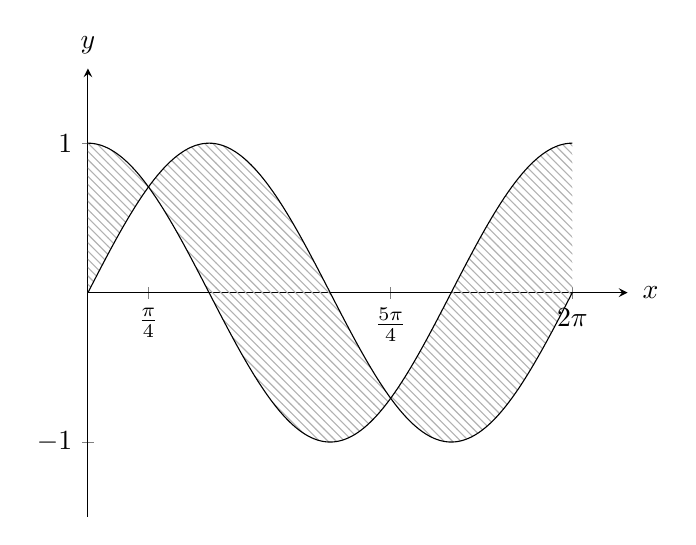
\begin{tikzpicture}
		\begin{axis}[
			scale = 1,
			axis x line = middle,
			axis y line = middle,
			xmin = 0,
			xmax = 7,
			ymin = -1.5,
			ymax = 1.5,
			xlabel = $x$,
			ylabel = $y$,
			xtick = {0.7854, 3.9270, 6.2831},
			xticklabels = {$\frac{\pi}{4}$, $\frac{5\pi}{4}$, $2\pi$},
			ytick = {-1, 1},
			yticklabels = {$-1$, $1$},
			every axis x label/.style = {
				at = {(ticklabel* cs:1.01)},
				anchor = west,
			},
			every axis y label/.style = {
				at = {(ticklabel* cs:1.01)},
				anchor = south,
			},
			restrict y to domain = -10:10
			]
			\addplot[
			name path = F,
			black,
			samples = 200,
			domain = 0:6.2831
			]{sin((x)r)};
			\addplot[
			name path = G,
			black,
			samples = 200,
			domain = 0:6.2831
			]{cos((x)r)};
			\addplot[
			pattern color = gray!60,
			pattern = north west lines
			] fill between [of = F and G];
		\end{axis}
	\end{tikzpicture}
	\caption{The area between $\sin(x)$ and $\cos(x)$ for $x$ between $0$ and $2 \pi$. }
	\label{lec12:areaexample}
\end{figure}

\begin{example}
	Find the area lying between $y = \sin(x)$ and $y = \cos(x)$ from $x = 0$ to $x = 2 \pi$, as seen in Figure \ref{lec12:positiveareas}.
	\begin{align*}
		A & = \int\limits_0^{\pi/4} \cos(x) - \sin(x) \, d x + \int\limits_{\pi/4}^{5 \pi/4} \sin(x) - \cos(x) \, d x + \int\limits_{5 \pi/4}^{2\pi} \cos(x) - \sin(x) \, d x \\
		  & = (\sin(x) - \cos(x)) \Big \rvert_0^{\pi/4} - (\cos(x) + \sin(x)) \Big \rvert_{\pi/4}^{5 \pi/4} + (\sin(x) - \cos(x)) \Big \rvert_{5\pi/4}^{2\pi}                 \\
		  & = (\sqrt{2} - 1) + (\sqrt{2} + \sqrt{2}) + (1 + \sqrt{2}) = 4 \sqrt{2}. \qedhere
	\end{align*}
\end{example}



\lecture[February 27, 2017]{Integration by Parts}

%!TEX root = ../lectures.tex

\topic{Integration by Parts}

Similar to how the method of substitution  is the chain rule baked into an integral, integration by parts is the product rule for derivatives combined with integrals.

Suppose $U$ and $V$ are two differentiable functions.
Then
\[
	\frac{d}{d x} (U(x) V(x)) = U(x) V'(x) + U'(x) V(x).
\]

\noindent
If we now integrate both sides, we get
\[
	U(x) V(x) = \int U(x) V'(x) \, d x + \int U'(x) V(x) \, d x,
\]
and if we rearrange we get
\[
	\int U(x) V'(x) \, d x = U(x) V(x) - \int U'(x) V(x) \, d x.
\]

\noindent
This is integration by parts, and it tells us that if we can view a function as the product of some function and the derivative of some other function, we might be able to integrate it more easily.

\begin{example}
	Compute $\int x e^x \, d x$.

	Consider $U(x) = x$ and $V'(x) = e^x$, whereby $U'(x) = 1$ and $V(x) = e^x$.
	We then get
	\[
		\int x e^x \, d x = x e^x - \int 1 \cdot e^x \, d x = x e^x - e^x + C = e^x (x - 1) + C.
	\]

	\noindent
	Note how we pick \emph{some} antiderivative of $V'$; instead of adding a constant term at that step we add one in the end, when we evaluate the indefinite integral in the right-hand side.
\end{example}

\noindent
This is a very powerful method of integration, allowing us to integrate some quite nasty functions.
One useful trick is to consider an integrand $f(x)$ as $1 \cdot f(x)$, which might simplify our problem greatly if $f$ is a function we know how to differentiate but not integrate.

\begin{example}
	Find $\int \ln(x) \, d x$.

	Let $U(x) = \ln(x)$ and $V'(x) = 1$, which means that $U'(x) = 1/x$ and $V(x) = x$.
	Thus
	\[
		\int \ln(x) \, d x = x \ln(x) - \int x \cdot \frac{1}{x} \, d x = x \ln(x) - x + C = x (\ln(x) -1) + C. \qedhere
	\]
\end{example}

\noindent
It is sometimes necessary to use integration by parts multiple times.

\begin{example}
	Find the indefinite integral of $x^2 \sin(x)$.

	Let $U(x) = x^2$ and $V'(x) = \sin(x)$, whereby $U'(x) = 2 x$ and $V(x) = - \cos(x)$.
	Using this we have
	\[
		\int x^2 \sin(x) \, d x = - x^2 \cos(x)  + 2 \int x \cos(x) \, d x.
	\]

	\noindent
	Now we use integration by parts once more in order to handle $x \cos(x)$.
	We pick $U(x) = x$ and $V'(x) = \cos(x)$, which gives us $U'(x) = 1$ and $V(x) = \sin(x)$.
	This means that
	\[
		\int x \cos(x) \, d x = x \sin(x) - \int 1 \cdot \sin(x) \, d x = x \sin(x) + \cos(x) + C,
	\]
	and putting everything together we have
	\begin{align*}
		\int x^2 \sin(x) \, d x &= - x^2 \cos(x)  + 2 \int x \cos(x) \, d x \\
		                        &= - x^2 \cos(x) + 2 x \sin(x) + 2 \cos(x) + D. \qedhere
	\end{align*}
\end{example}

\noindent
So far, in the examples involving a polynomial factor, we've chosen this as the part we differentiate.
This is not always the best idea.

\begin{example}
	Integrate $x \arctan(x)$.

	Since we probably don't have the integral of $\arctan(x)$ in our heads\footnote{Though we could have; try using integration by parts on it the same way we did with $\ln(x)$.} we try differentiating $\arctan$ instead, since we know how to do that.

	Thus $U(x) = \arctan(x)$ and $V'(x) = x$ whereby $U'(x) = 1 / (1 + x^2)$ and $V(x) = x^2 / 2$.
	Therefore
	\begin{align*}
		\int x \arctan(x) \, d x &= \frac{1}{2} x^2 \arctan(x) - \frac{1}{2} \int \frac{1}{1 + x^2} \cdot x^2 \, d x \\
		                         &= \frac{1}{2} x^2 \arctan(x) - \frac{1}{2} \int 1 - \frac{1}{1 + x^2} \, d x \\
		                         &= \frac{1}{2} x^2 \arctan(x) - \frac{1}{2} x + \frac{1}{2} \arctan(x) + C \\
														 &= \frac{1}{2} ((x^2 + 1) \arctan(x) - x) + C. \qedhere
	\end{align*}
\end{example}

\noindent
Another useful trick is to perform integration by parts several times until our integrand reappears in the right-hand side.

\begin{example}
	Compute
	\[
		I = \int (\sec(x))^3 \, d x.
	\]

	\noindent
	Being slightly tricky we recall that the derivative of $\tan(x)$ is $(\sec(x))^2$, so we split the integrand into $\sec(x) (\sec(x))^2$, whereby $U(x) = \sec(x)$ and $V'(x) = (\sec(x))^2$.
	Then $U'(x) = \sec(x) \tan(x)$ (feel free to verify) and $V(x) = \tan(x)$.
	Thus
	\begin{align*}
		I &= \sec(x) \tan(x) - \int \sec(x) (\tan(x))^2 \, d x \\
		  &= \sec(x) \tan(x) - \int \sec(x) ((\sec(x))^2 - 1) \, d x \\
			&= \sec(x) \tan(x) - \underbrace{\int (\sec(x))^3 \, d x}_{=\, I} + \int \sec(x) \, d x,
	\end{align*}
	so
	\[
		2 I = \sec(x) \tan(x) + \int \sec(x) \, d x.
	\]

	\noindent
	It remains to compute the integral of $\sec(x)$.
	To do so we come up with the brilliant idea of multiplying and dividing by $u(x) = \sec(x) + \tan(x)$, because $u'(x) = \tan(x) \sec(x) + (\sec(x))^2 = \sec(x) (\sec(x) + \tan(x))$, whereby
	\begin{align*}
		\int \sec(x) \, d x &= \int \frac{\sec(x) (\sec(x) + \tan(x))}{\sec(x) + \tan(x)} \, d x = \int \frac{1}{u} \, d u \\
		                    &= \ln\abs{u} + C = \ln\abs{\sec(x) + \tan(x)} + C.
	\end{align*}

	\noindent
	Therefore
	\[
		I = \frac{1}{2} (\sec(x) \tan(x) + \ln\abs{\sec(x) + \tan(x)}) + D. \qedhere
	\]
\end{example}

\begin{example}
	Let $a, b \neq 0$ be constants and find
	\[
		I = \int e^{a x} \cos(b x) \, d x.
	\]

	\noindent
	We use $U(x) = e^{a x}$ and $V'(x) = \cos(bx)$, whence $U'(x) = a e^{a x}$ and $V(x) = \sin(b x) / b$.
	Then
	\begin{align*}
		I &= \frac{1}{b} e^{a x} \sin(b x) - \frac{a}{b} \int e^{a x} \sin(b x) \, d x \\
		  &= \frac{1}{b} e^{a x} \sin(b x) - \frac{a}{b} \Big ( - \frac{1}{b} e^{a x} \cos(b x) + \frac{a}{b} \int e^{a x} \cos(b x) \, d x \Big ) \\
			&= \frac{1}{b} e^{a x} \sin(b x) + \frac{a}{b^2} e^{a x} \cos(b x) - \frac{a^2}{b^2} I.
	\end{align*}

	\noindent
	Rearranging we get
	\[
		\Big ( 1 + \frac{a^2}{b^2} \Big ) I = \frac{1}{b} e^{a x} \Big ( \sin(b x) + \frac{a}{b} \cos(b x) \Big ) + C,
	\]
	meaning that
	\[
		I = \int e^{a x} \cos(b x) \, d x = \frac{b e^{a x} \sin(b x) + a e^{a x} \cos(b x)}{a^2 + b^2} + D.
	\]

	\noindent
	Note that this works because we pick the same $U(x)$ both times.
	If we didn't, we'd have gotten
	\[
		I = \frac{1}{b} e^{a x} \sin(b x) - \frac{1}{b} e^{a x} \sin(b x) + I,
	\]
	which is just a complicated way of writing $0 = 0$.
\end{example}

\topic{Integrating Rational Functions}

We will now spend some time studying integrals of the form
\[
	\int \frac{P(x)}{Q(x)} \, d x,
\]
where $P$ and $Q$ are polynomials.

When doing this, we will almost always assume that $\deg(P(x)) < \deg(Q(x))$, since if it is not the case, we just perform polynomial division.

\begin{example}
	Compute $I = \int \frac{x^3 + 3 x^2}{x^2 + 1} \, d x$.

	\smallskip

	First we perform the polynomial division.
	\begin{figure}[H]
		\centering
		\polylongdiv{x^3 + 3 x^2}{x^2 + 1}
	\end{figure}

	\noindent
	Therefore
	\[
		\frac{x^3 + 3 x^2}{x^2 + 1} = (x + 3) + \frac{- x - 3}{x^2 + 1},
	\]
	whereby
	\begin{align*}
		I &= \int x + 3 \, d x - \int \frac{x}{x^2 + 1} \, d x - 3 \int \frac{d x}{x^2 + 1} \\
		  &= \frac{1}{2} x^2 + 3 x - \frac{1}{2} \ln(x^2 + 1) - 3 \arctan(x) + C. \qedhere
	\end{align*}
\end{example}

\noindent
Therefore in what follows the degree of the numerator will be less than the degree of the denominator, since otherwise we just perform polynomial division and end up in that situation anyway.

There are then a few cases to consider.

Suppose $\deg(Q(x)) = 1$.
Then $Q(x) = a x + b$, with $a \neq 0$, and $\deg(P(x)) = 0$, so $P(x) = c$.
We substitute $u(x) = a x + b$, whereby $d u = a \, d x$, and
\[
	\int \frac{c}{a x + b} \, d x = \frac{c}{a} \int \frac{1}{u} \, d u = \frac{c}{a} \ln\abs{u} + C = \frac{c}{a} \ln\abs{a x + b} + C.
\]

\noindent
Now suppose $Q(x)$ is quadratic, i.e. $Q(x) = A x^2 + B x + C$, with $A \neq 0$.
Then by completing the square and making some simple substitution we can always get it on the form $x^2 + a^2$ or $x^2 - a^2$, multiplied by some constant  we don't bring into the integral anyway.
Thus since $P(x) = \alpha x + \beta$, there are four types of integrals to consider:
\begin{alignat*}{5}
	\int \frac{x}{x^2 + a^2} \, d x &= \frac{1}{2} \ln(x^2 + a^2) + C, \qquad                  && \int \frac{x}{x^2 - a^2} \, d x &&= \frac{1}{2} \ln\abs{x^2 - a^2} + C, \\
	\int \frac{1}{x^2 + a^2} \, d x &= \frac{1}{a} \arctan\Big (\frac{x}{a} \Big ) + C, \qquad && \int \frac{1}{x^2 - a^2} \, d x &&= \frac{1}{2 a} \ln\abs[\Big]{\frac{x - a}{x + a}} + C.
\end{alignat*}

\noindent
The first three of these are known or obvious, however the forth one is trickier.
We do the following:
\[
	\frac{1}{x^2 - a^2} = \frac{1}{(x - a)(x + a)} = \frac{A}{x - a} + \frac{B}{x + a} = \frac{A x + A a + B x - B a}{x^2 - a^2},
\]
meaning that $A x + A a + B x - B a = (A + B) x + (A - B) a = 1$, so
\[
	\begin{cases}
		A + B = 0 \\
		A a - B a = 1
	\end{cases} \Longleftrightarrow~
	\begin{cases}
		A = 1 / (2 a) \\
		B = - 1 / (2 a),
	\end{cases}
\]
and therefore
\begin{align*}
	\int \frac{d x}{x^2 - a^2} &= \frac{1}{2 a} \int \frac{d x}{x - a} - \frac{1}{2 a} \int \frac{d x}{x + a} \\
	                           &= \frac{1}{2 a} \ln\abs{x - a} - \frac{1}{2 a} \ln\abs{x + a} + C = \frac{1}{2 a} \ln\abs[\Big]{\frac{x - a}{x + a}} + C.
\end{align*}

\noindent
What we just did is called \keyword{partial fraction decomposition}\index{partial fraction decomposition}.

In general, if $Q(x) = (x - \alpha_1)(x - \alpha_2) \cdots (x - \alpha_n)$, where all $\alpha_i$ are different, then there always exist, for $P(x)$ of smaller degree, $A_1, A_2, \ldots, A_n$ such that
\[
	\frac{P(x)}{Q(x)} = \frac{A_1}{x - \alpha_1} + \frac{A_2}{x - \alpha_2} + \ldots + \frac{A_n}{x - \alpha_n}.
\]

\noindent
(We won't prove that this always works here; that belongs in an algebra course. However the curious student may find the details of the proof in, for example, \cite[Section 4.4]{Nicholson1999}.)

We can find the $A_i$ either by the sytem of equations as before, or by noting that if we multiply $P(x) / Q(x)$ by $x - \alpha_j$, we get
\[
	A_1 \frac{x - \alpha_j}{x - \alpha_1} + \ldots + A_{j - 1} \frac{x - \alpha_j}{x - \alpha_{j - 1}} + A_j + A_{j + 1} \frac{x - \alpha_j}{x - \alpha_{j + 1}} + \ldots + A_n \frac{x - \alpha_j}{x - \alpha_n}.
\]

\noindent
Thus when $x = a_j$, all but $A_j$ disappear, meaning that
\[
	A_j = \lim_{x \to \alpha_j} (x - \alpha_j) \frac{P(x)}{Q(x)}.
\]

\noindent
This works, with one caveat: if there's a repeated factor, we need to be careful:

\begin{example}
	Find
	\[
		I = \int \frac{1}{x (x - 1)^2} \, d x.
	\]

	\noindent
	The correct ansatz in this case is
	\[
		\frac{1}{x (x - 1)^2} = \frac{A}{x} + \frac{B}{x - 1} + \frac{C}{(x - 1)^2},
	\]
	so we have $A(x^2 - 2 x + 1) + B(x^2 - x) + C x = 1$, from which we glean
	\[
		\begin{cases}
			A + B = 0 \\
			-2 A - B + C = 0 \\
			A = 1
		\end{cases} \Longleftrightarrow~
		\begin{cases}
			A = 1 \\
			B = -1 \\
			C = 1,
		\end{cases}
	\]
	meaning that
	\begin{align*}
		I &= \int \frac{1}{x} \, d x - \int \frac{1}{x - 1} \, d x + \int \frac{1}{(x - 1)^2} \, d x \\
		  &= \ln\abs{x} - \ln\abs{x - 1} - \frac{1}{x - 1} + C = \ln\abs[\Big]{\frac{x}{x - 1}} - \frac{1}{x - 1} + C. \qedhere
	\end{align*}
\end{example}


\noindent
If $Q(x)$ cannot be factored into linear terms, the ansatz changes a little.
We'd use e.g.
\[
	\frac{x^2 + 2}{x (2 x^2 + 1)^2} = \frac{A}{x} + \frac{B x + C}{2 x^2 + 1} + \frac{D x + E}{(2 x^2 + 1)^2}.
\]









% List of references.
\clearpage
\begin{thebibliography}{99999}
	\bibitem[Ad13]{Adams2013} R.\,A. Adams.
	\emph{Calculus: A Complete Course}.
	Prentice-Hall,
	1136 pages,
	8th revised edition,
	2013.
\end{thebibliography}

% Make a pretty index.
\clearpage
\printindex

\end{document}
